%-----------------------------------------------------------------------
% Beginning of chapter.tex
%-----------------------------------------------------------------------
%
%  This is a sample file for use with AMS-LaTeX.  It provides an example
%  of how to set up a file for a book to be typeset with AMS-LaTeX.
%
%  This is the driver file.  Separate chapters should be included at
%  the end of this file.
%
%  ***** DO NOT USE THIS FILE AS A STARTER FOR YOUR BOOK. *****
%  Follow the guidelines in the file chapter.template.
%
%%%%%%%%%%%%%%%%%%%%%%%%%%%%%%%%%%%%%%%%%%%%%%%%%%%%%%%%%%%%%%%%%%%%%%%%

\documentclass{amsbook}

\usepackage{amsmath,amssymb,amsthm,amsfonts,enumerate, mathrsfs, mathtools, appendix}
\usepackage{relsize}
\usepackage{stmaryrd}
\usepackage{esint}
\usepackage{xcolor}
\usepackage{graphicx}
\usepackage{framed}
\usepackage[%colorlinks=false,   
colorlinks=true,
linkcolor=blue,
filecolor=blue,
urlcolor=red,
citecolor=magenta]{hyperref}
\usepackage{cleveref}
%------------------------------------- hyper  


\includeonly{preface,chap1,chap2,chap3,chap4,chap5,chap6,appendix,index}

\newtheorem{theorem}{Theorem}[chapter]
\newtheorem{lemma}[theorem]{Lemma}
\newtheorem{proposition}[theorem]{Proposition}
\newtheorem{corollary}[theorem]{Corollary}

\theoremstyle{definition}
\newtheorem{definition}[theorem]{Definition}
\newtheorem{example}[theorem]{Example}
\newtheorem{exercise}[theorem]{Exercise}

\theoremstyle{remark}
\newtheorem{remark}[theorem]{Remark}

\newtheorem{assumption}{Assumption}

\numberwithin{section}{chapter}
\numberwithin{equation}{chapter}

%    Absolute value notation
\newcommand{\abs}[1]{\lvert#1\rvert}

%    Blank box placeholder for figures (to avoid requiring any
%    particular graphics capabilities for printing this document).
\newcommand{\blankbox}[2]{%
  \parbox{\columnwidth}{\centering
%    Set fboxsep to 0 so that the actual size of the box will match the
%    given measurements more closely.
    \setlength{\fboxsep}{0pt}%
    \fbox{\raisebox{0pt}[#2]{\hspace{#1}}}%
  }%
}

%-------------------------------------mark conastant
\newcounter{counterConstant} 
\newcommand{\const}[1]{	\addtocounter{counterConstant}{1}
\edef#1{\arabic{counterConstant}}
}
%-------------------------------------

%-------------------------------------abbreviation
\def\cA{{\mathcal A}}
\def\cB{{\mathcal B}}
\def\cC{{\mathcal C}}
\def\cD{{\mathcal D}}
\def\cE{{\mathcal E}}
\def\cF{{\mathcal F}}
\def\cG{{\mathcal G}}
\def\cH{{\mathcal H}}
\def\cI{{\mathcal I}}
\def\cJ{{\mathcal J}}
\def\cK{{\mathcal K}}
\def\cL{{\mathcal L}}
\def\cM{{\mathcal M}}
\def\cN{{\mathcal N}}
\def\cO{{\mathcal O}}
\def\cP{{\mathcal P}}
\def\cQ{{\mathcal Q}}
\def\cR{{\mathcal R}}
\def\cS{{\mathcal S}}
\def\cT{{\mathcal T}}
\def\cU{{\mathcal U}}
\def\cV{{\mathcal V}}
\def\cW{{\mathcal W}}
\def\cX{{\mathcal X}}
\def\cY{{\mathcal Y}}
\def\cZ{{\mathcal Z}}

\def\mA{{\mathbb A}}
\def\mB{{\mathbb B}}
\def\mC{{\mathbb C}}
\def\mD{{\mathbb D}}
\def\mE{{\mathbb E}}
\def\mF{{\mathbb F}}
\def\mG{{\mathbb G}}
\def\mH{{\mathbb H}}
\def\mI{{\mathbb I}}
\def\mJ{{\mathbb J}}
\def\mK{{\mathbb K}}
\def\mL{{\mathbb L}}
\def\mM{{\mathbb M}}
\def\mN{{\mathbb N}}
\def\mO{{\mathbb O}}
\def\mP{{\mathbb P}}
\def\mQ{{\mathbb Q}}
\def\mR{{\mathbb R}}
\def\mS{{\mathbb S}}
\def\mT{{\mathbb T}}
\def\mU{{\mathbb U}}
\def\mV{{\mathbb V}}
\def\mW{{\mathbb W}}
\def\mX{{\mathbb X}}
\def\mY{{\mathbb Y}}
\def\mZ{{\mathbb Z}}

\def\bA{{\mathbf A}}
\def\bB{{\mathbf B}}
\def\bC{{\mathbf C}}
\def\bD{{\mathbf D}}
\def\bE{{\mathbf E}}
\def\bF{{\mathbf F}}
\def\bG{{\mathbf G}}
\def\bH{{\mathbf H}}
\def\bI{{\mathbf I}}
\def\bJ{{\mathbf J}}
\def\bK{{\mathbf K}}
\def\bL{{\mathbf L}}
\def\bM{{\mathbf M}}
\def\bN{{\mathbf N}}
\def\bO{{\mathbf O}}
\def\bP{{\mathbf P}}
\def\bQ{{\mathbf Q}}
\def\bR{{\mathbf R}}
\def\bS{{\mathbf S}}
\def\bT{{\mathbf T}}
\def\bU{{\mathbf U}}
\def\bV{{\mathbf V}}
\def\bW{{\mathbf W}}
\def\bX{{\mathbf X}}
\def\bY{{\mathbf Y}}
\def\bZ{{\mathbf Z}}

\def\sA{{\mathscr A}}
\def\sB{{\mathscr B}}
\def\sC{{\mathscr C}}
\def\sD{{\mathscr D}}
\def\sE{{\mathscr E}}
\def\sF{{\mathscr F}}
\def\sG{{\mathscr G}}
\def\sH{{\mathscr H}}
\def\sI{{\mathscr I}}
\def\sJ{{\mathscr J}}
\def\sK{{\mathscr K}}
\def\sL{{\mathscr L}}
\def\sM{{\mathscr M}}
\def\sN{{\mathscr N}}
\def\sO{{\mathscr O}}
\def\sP{{\mathscr P}}
\def\sQ{{\mathscr Q}}
\def\sR{{\mathscr R}}
\def\sS{{\mathscr S}}
\def\sT{{\mathscr T}}
\def\sU{{\mathscr U}}
\def\sV{{\mathscr V}}
\def\sW{{\mathscr W}}
\def\sX{{\mathscr X}}
\def\sY{{\mathscr Y}}
\def\sZ{{\mathscr Z}}

\def\l{\left}
\def\r{\right}
\def\<{\langle}
\def\>{\rangle}

\def\geq{\geqslant}
\def\leq{\leqslant}

\def\1{{\mathbf{1}}}
\def\p{\partial}
\def\d{\text{\rm{d}}}
\def\e{\mathrm{e}}
\def\eps{\varepsilon}
\def\Re{{\mathrm{Re}}}
\def\Im{{\mathrm{Im}}}
\def\var{{\mathrm{var}}}
\def\HS{{\mathrm{\tiny HS}}}
\def\div{\mathord{{\rm div}}}
\def\osc{\mathop{{\rm osc}}}
\def\sgn{\textit{\rm sgn}}
\def\Law{{\mathord{{\rm Law}}}}
\def\esssup{\mathop{\mathrm{ess\,sup}}}
\def\essinf{\mathop{\mathrm{ess\,inf}}}

%-------------------------------------

\begin{document}
\frontmatter
\title{An Introduction to Diffusion Processes}

%    Information for first author
\author{Guohuan Zhao}
%    Address of record for the research reported here
\address{The Academy of Mathematics and Systems Science of Chinese Academy of Sciences, Beijing 100190, China}
%    Current address
%\curraddr{Department of Mathematics and Statistics,
%Case Western Reserve University, Cleveland, Ohio 43403}
\email{gzhao@amss.ac.cn}
%    \thanks will become a 1st page footnote.
%\thanks{}
%    Information for second author
\date{\today}
%\subjclass[2020]{Primary 54C40, 14E20;\\Secondary 46E25, 20C20}
%\keywords{\texttt{amsbook}, AMS-\LaTeX}

\maketitle

\setcounter{page}{4}
\tableofcontents

%-----------------------------------------------------------------------------
% Beginning of preface.tex
%-----------------------------------------------------------------------------
%
% AMS-LaTeX 1.2 sample file for a monograph, based on amsbook.cls.
% This is a data file input by chapter.tex.
%%%%%%%%%%%%%%%%%%%%%%%%%%%%%%%%%%%%%%%%%%%%%%%%%%%%%%%%%%%%%%%%%%%%%%%%

\chapter*{Preface}

The primary motivation for writing this lecture note is to introduce graduate students to the historical background, modern mathematical treatment, and certain analytical applications of {\bf diffusion processes}.  During the preparation, the main reference was Richard Bass's book {\em Diffusions and Elliptic Operators}, which provided a solid foundation and valuable insights.

Given the time constraint of a ten-week short course, it is impossible to cover all aspects of this rich subject in depth. Therefore, I have selected a number of fundamental and interesting topics and reorganized them in my own way to form the content of these notes. My hope is that this material will offer a clear and engaging entry point into the theory of diffusion processes for students encountering it for the first time.

\aufm{Guohuan Zhao}

%-----------------------------------------------------------------------------
% End of preface.tex
%-----------------------------------------------------------------------------


\mainmatter

%-----------------------------------------------------------------------
% Beginning of chap1.tex
%-----------------------------------------------------------------------
%
%  AMS-LaTeX sample file for a chapter of a monograph, to be used with
%  an AMS monograph document class.  This is a data file input by
%  chapter.tex.
%
%  Use this file as a model for a chapter; DO NOT START BY removing its
%  contents and filling in your own text.
% 
%%%%%%%%%%%%%%%%%%%%%%%%%%%%%%%%%%%%%%%%%%%%%%%%%%%%%%%%%%%%%%%%%%%%%%%%

%\part{This is a Part Title Sample}

\chapter{Construction of Diffusion processes I}


\section{Brownian Motion}
The {\em Brownian motion} is a continuous stochastic process characterized by independent increments that follow a normal distribution. It is widely used to model the irregular motion of tiny particles suspended in a fluid. As one of the fundamental concepts in stochastic analysis, Brownian motion serves as a cornerstone for understanding more complicate stochastic processes.

In physics, Brownian motion was discovered in 1827 by the British botanist Robert Brown. While observing pollen particles suspended in water under a conventional microscope, he noticed their irregular motion. Since 1860, numerous scientists have studied this phenomenon and identified the following key characteristics of Brownian motion: 
\begin{enumerate}
    \item The motion of the particles consists of translation and rotation; %, appearing very irregular, and their trajectories are almost everywhere without tangents;
    \item The movements of the particles are apparently uncorrelated, even when the particles approach each other to distances smaller than their diameters;
    \item The smaller the particles, the lower the viscosity of the liquid, or the higher the temperature, the more active the motion of the particles;
    \item The composition and density of the particles have no effect on their motion;
    \item The motion of the particles never stops.
\end{enumerate}

In 1905, Einstein proposed a related theory. His theory has two parts: the first part defines the diffusion equation for Brownian particles, where the diffusion coefficient is related to the mean square displacement of the Brownian particles, and the second part describes the relationship between the diffusion coefficient and measurable physical quantities. Here we briefly introduce the first part: determining the distance a Brownian particle moves in a given time. Classical mechanics cannot determine this distance because a Brownian particle will be subjected to a large number of collisions, approximately \(10^{14}\) collisions per second. Einstein considered the position of the particle in space at time \( t \) as a random variable \( X_t \), and let \( \rho(t,x) \) be the density of \( X_t \). Assume \( \tau_B \) is the relaxation time, and \( \Delta t \gg \tau_B \). The increment \( X_{t+\Delta t} - X_t \) over the time interval \( \Delta t \) is also a random variable, and its probability density is assumed to be \( \varphi_{\Delta t} \) (depending only on \( \Delta t \)). For a homogeneous liquid, we can naturally assume that \( \varphi_{\Delta t} \) is rotationally symmetric. Using Taylor expansion:
\begin{align*}
    \rho(t,x) + \partial_t \rho(t,x) \Delta t \approx & \rho(t + \Delta t, x) = \int_{\mathbb{R}^3} \rho(t,x-y) \varphi_{\Delta t}(y) \d y\\
    \approx& \rho(t,x) \int_{\mathbb{R}^3} \varphi_{\Delta t}(y) \d y - \nabla \rho(t,x) \cdot \int_{\mathbb{R}^3} y \varphi_{\Delta t}(y) \d y\\
    &+ \frac{1}{2} \partial_{y_iy_j}^2 \rho(t,x) \int_{\mathbb{R}^3} y_iy_j \varphi_{\Delta t}(y) \d y\\
    =& \rho(t,x) + \frac{1}{2} \int_{\mathbb{R}^3} |y|^2 \varphi_{\Delta t}(y) dy \Delta \rho(t,x).
\end{align*}
Therefore,
\[
\partial_t \rho = \frac{\int_{\mathbb{R}^3} |y|^2 \varphi_{\Delta t}(y) dy}{2\Delta t} \Delta \rho.
\]

From both theoretical and experimental perspectives, it is reasonable to assume that \( \nu = \frac{1}{2\Delta t} \int_{\mathbb{R}^3} |y|^2 \varphi_{\Delta t}(y) dy \) is a constant, called the diffusion coefficient of the Brownian particle. Thus, the above equation can be written as:

\[
\partial_t \rho = \nu \Delta \rho, \quad \rho(0,x) = f(x).
\]

The solution to this heat equation is:

\[
\rho(t,x) = \int_{\mathbb{R}^3} \frac{1}{(4\pi\nu t)^{3/2}} e^{-\frac{(x-y)^2}{4\nu t}} f(y) dy.
\]

From this, we obtain that if \( X_0 = x \), then the distribution of \( X_t \) is a standard Gaussian distribution. The second part of Einstein's theory relates the diffusion constant to physically measurable quantities, such as the mean square displacement of the particle over a given time interval. This result allows for the experimental determination of Avogadro's number and, consequently, the size of molecules. However, we will not discuss this further here.

\subsection{Mathematical Definition of Brownian Motion}

Note that Einstein did not explicitly establish a mathematical model for Brownian motion. This problem was solved by Wiener. 

\begin{definition}\label{Def:BM}
    \( (W_t)_{t\geq 0} \) is a stochastic process satisfying:
    \begin{enumerate}
        \item {\bf Stationary independent increments and Gaussian property}: For \( t > s \), the increment \( W_t - W_s \) follows a normal distribution with mean 0 and variance \( (t-s)I_{d\times d} \), and the increment \( W_t - W_s \) is independent of the process \( (W_u)_{0\leq u\leq s} \) before time \( s \);
        \item {\bf Path continuity}: \( (W_t)_{t\geq 0} \) is almost surely continuous;
    \end{enumerate}
    Usually, we assume \( W_0 = 0 \), in which case, \(W\) is called standard Brownian motion.
\end{definition} 
Of course, a natural mathematical question is whether such a stochastic process exists. 

%In fact, we can define a probability measure \( \mathbb{P} \) on \( \Omega = C(\mathbb{R}^+; \mathbb{R}) \) such that the canonical process \( W_t(\omega) = \omega \) on \( \Omega \) is a standard Brownian motion, and it can be proven that for any \( \alpha \in (0,1/2) \):
% \[
% \mathbb{P}(\|W\|_{C^\alpha([0,T];\mathbb{R})} < \infty) = 1,
% \]
% and
% \[
% \mathbb{P}\left(\limsup_{t \to t_0} \frac{|W_t - W_{t_0}|}{\sqrt{t-t_0}} < \infty\right) = 0.
% \]
\medskip

A stochastic process defined on $(\Omega, \cF, \bP)$ taking value in a measurable space $(E, \cE)$ can be understood in various ways. It involves a collection of random variables $X_t\in E$ indexed by a parameter set $\bT$ (usually, $\bT=\mN$ or $\mR_+$), where $X_t$ is a measurable map from $(\Omega, \cF,\bP)$ to $(E, \cE)$ for each $t\in \bT$. The parameter set $\bT$ typically represents time and can be discrete or continuous. The process can also be regard as a measurable map from $(\Omega, \cF, \bP)$ to the space of functions $E^\bT$. The Kolmogorov $\sigma$-field on $E^{\bT}$ is the smallest $\sigma$-field making the projections $\pi_t: E^{\bT} \ni f\mapsto f(t)\in E$ measurable. This definition ensures that a random map  $\Omega \ni \omega \mapsto X_{\cdot}(\omega) \in E^{\bT}$ is measurable if its component random variables $X_t:\Omega \to E$ are measurable for all $t\in \bT$. Therefore, the mapping $\omega\mapsto X_{\cdot}(\omega)$ induces a measure on $(E^{\bT}, \cE^{\bT})$ denoted by $\mP$. The underlying probability model $(\Omega, \cF, \bP)$ is replaceable by the canonical model $(\mP, E^{\bT}, \cE^{\bT})$ with a specific choice of $X_t(f)=\pi_t(f)=f(t)$. In simpler terms, a stochastic process is just a probability measure $\mP$ on $(E^{\bT}, \cE^{\bT})$.
	
Another point of view is that the only relevant objects are the joint distributions of $(X_{t_1}, X_{t_2}, \cdots , X_{t_n})$ for every $n$ and every finite subset $I = (t_1, t_2, ... , t_n)$ of $\bT$. These can be specified as probability measures $\mu_{I}$ on $\mR^n$. These $\mu_{I}$ cannot be totally arbitrary. If we allow different permutations of the same set, so that $I$ and $I'$ are permutations of each other then $\mu_I$ and $\mu_{I'}$ should be related by the same permutation. If $I\subseteq I'$, then we can obtain the joint distribution of $(X_t)_{t\in I}$ by projecting the joint distribution of $(X_t)_{t\in I'}$ from $\mR^{n'}$ to $\mR^{n}$ where $n$ and $n'$ are the cardinalities of $I$ and $I'$ respectively. A stochastic process can then be viewed as a family $(\mu_I)$ of distributions on various finite dimensional spaces that satisfy the consistency conditions. A theorem of Kolmogorov says that this is not all that different. Any such consistent family arises from a $\mP$ on $(E^{{\bT}} , \cE^{\bT})$ which is uniquely determined by the family $(\mu_I)$.

\begin{definition}
    We say A measurable space \((E, \cE)\) is said to be standard if there exists a Polish space \(X\) such that \((E,\cE)\) is isomorphic (as a measurable space) to \((X,\cB(X))\). 
\end{definition}

\begin{theorem}[Kolmogorov's consistency Theorem, cf. \cite{Yan2021Measure}]\label{Thm:K1}
    Let $E$ be a standard measure space. Assume that we are given for every $t_1,...,t_n\in \bT$ a probability measure  $\mu_{t_1\cdots t_n}$ on $E^n$, and that these probability measures satisfy:
	\begin{enumerate}[(i)]
		\item for each $\tau\in S_n$ and $A_i \in \cE$, 
		$$
			\mu_{t_1\cdots t_n} (A_1 \times ... \times A_n)=\mu_{t_{\tau(1)}\cdots t_{\tau(n)}} (A_{\tau(1)} \times ... \times A_{\tau(n)});
		$$
		\item for each $A_i \in \cE$, 
		$$
			\mu_{t_1\cdots t_n} (A_1 \times ... \times A_{n-1} \times E)=\mu_{t_1\cdots t_{n-1}} (A_1 \times ... \times A_{n-1}). 
		$$
	\end{enumerate}
    Then, there is a unique probability measure $\bP$ on $(E^{\bT}, \cE^{\bT})$ such that for $t_1,...,t_n \in \bT, A_1,...,A_n \in \cE$: $\bP (f(t_1) \in A_1,...,f(t_n) \in A_n)=\mu_{t_1,...,t_n}(A_1 \times ... \times A_n)$. 
\end{theorem}
	
	
Let \(\bT=\mR_+\) and \(E\) be a Polish space. By \Cref{Thm:K1}, we can define a probability measure $\mP$ on $E^{\mR_+}$ such that the canonical process $X_t(f)=f(t)$ satisfies the conditions in \Cref{Thm:K1}. However, whether the measure is concentrated on the space of continuous functions is not a simple question. In fact, since $\bT=\mR_+$ is uncountable the space of bounded functions, continuous functions, etc., are \textbf{not} measurable sets of $E^{\mR_+}$. They do not belong to the natural $\sigma$-field. Essentially, in probability theory, the rules involve only a countable collection of sets at one time, and any information that involves the values of an uncountable number of measurable functions is beyond reach. There is an intrinsic reason for this. In probability theory, we can always change the values of a random variable on a set of measure $0$, and we have not changed anything significant. Since we are allowed to mess up each function on a set of measure $0$, we have to assume that each function has indeed been messed up on a set of measure 0. If we are dealing with a countable number of functions, the `mess up' has occurred only on the countable union of these individual sets of measure $0$, which, by the properties of a measure, is again a set of measure $0$. On the other hand, if we are dealing with an uncountable set of functions, then these sets of measure $0$ can possibly gang up on us.
	
Often, we aim to find a version of stochastic process with continuous trajectories,  or equivalently, to establish a measure $\mP$ on $C(\mR_+; \mR^d)$ with the natural $\sigma$-field. However, this is not always achievable. We are looking for sufficient conditions on the finite dimensional distributions $(\mu_I)$ to ensure the existence of $\mP$ on $C(\mR_+; \mR^d)$.
	
\begin{theorem}[Kolmogorov]\label{Thm:K2}
    Let $I=[0,T]$, and let $p>1$ and $\beta\in(1/p,1)$. Assume $(Y_t\in \mR^d)_{t\in I}$ satisfies  
    \begin{equation}\label{eq:moment}
        \bE |Y_s-Y_t|^p \leq c |t-s|^{1+\beta p}, \quad ~\forall t,s\in I. 
    \end{equation}
    Then there exists a version of $Y$, say $X$ (for each \(t\in I\), $\bP(X_t=Y_t)=1$), such that  
    \[
        \bP\l(\sup_{t\in I}\frac{|X_t-X_s|}{|t-s|^\alpha}\leq K\r) =1, 
    \]
    where $\alpha\in (0,\beta-1/p)$, $K=K(\alpha,\beta,p,c,I,\omega)$ and $\bE K^p<\infty$. 
\end{theorem}
\begin{proof}
    Regard $Y$ as a measurable function from  $\Omega\times I$ to $\mR^d$. By Lemma \ref{Le:GRRI} below, there is a null set $\cN\subseteq \Omega$ and a measurable function $X: \Omega\times I \to \mR^d$, such that for each $\omega\notin \cN$, 
    \[
	\sL^1\l(\{ t\in I: X_t(\omega)\neq Y_t(\omega)\}\r)=0, 
    \]
    and $X(\omega)_{\cdot}$ is a continuous function. Moreover, 
    \[
    \|X_{\cdot}(\omega)\|_{C^{\alpha}(I)}\lesssim  K(\omega):= \l(\iint_{I\times I} \frac{|Y_t(\omega)-Y_s(\omega)|^p}{|t-s|^{2+\alpha p}}\, \d s \d t\r)^{1/p}\in L^p(\bP).
    \]
    By Fubini theorem, there exists a $\sL^1$-null set $N\subseteq I$, such that for each $t\notin N$, $\bP(X_t\neq Y_t)=0$. For any $t_0\in N$, by \eqref{eq:moment}, one can see that $Y_{t_n} \xrightarrow[I\backslash N \ni t_n \to t_0]{\bP} Y_{t_0}$. On the other hand, $Y_{t_n}\overset{\mbox{a.s}}{=}X_{t_n}\to X_{t_0}$, so we have $X_{t_0}\overset{\mbox{a.s}}{=}Y_{t_0}$. Therefore, $X$ is a continuous version of $Y$. 
\end{proof}

\begin{lemma}[Fractional Sobolev inequality]\label{Le:GRRI}
    Let $R>0$, $p>n$ and $s\in (n/p,1)$. Let $f:B_R\to \mR^d$ be a measurable function. Assume 
    \begin{align*}
	\iint_{B_R\times B_R}\frac{|f(x)-f(y)|^p}{|x-y|^{n+sp}}\, \d x \d y<\infty. 
    \end{align*}
    Then there exists a version of $f$, say $\tilde f$, such that 
    \begin{equation}
	\sup_{x,y\in B_R}\frac{|\tilde f(x)-\tilde f(y)|}{|x-y|^{s-\frac{n}{p}}}\leq C \l(\iint_{B_R\times B_R} \frac{|f(x)-f(y)|^p}{|x-y|^{n+sp}}\, \d x\d y\r)^{1/p}, 
    \end{equation}
    Here $C$ only depends on $n,s,p$ and $R$. 
\end{lemma}
	
Thanks to \Cref{Thm:K2} and the discussion after  \Cref{Thm:K1}, we can first construct a probability measure \(\bP\) on \(\Omega=(\mR^d)^{\mR_+}\) such that 
\begin{align*}
    &\bP(Y_{t_1}\in A_1,\cdots, Y_{t_n}\in A_n)\\
    =&\int_{A_1}\cdots\int_{A_n} p_{t_1}(x_1) p_{t_2-t_1}(x_1-x_2) \cdots p_{t_n-t_{n-1}}(x_{n-1}-x_n) \d x_1\cdots \d x_n,  
\end{align*}
where \(Y_t(\omega)=\omega\) is the canonical process, and \(p_t(x)=(2\pi t)^{-\frac{d}{2}} \exp (-|x|^2/(2t))\). Then using \Cref{Thm:K2}, one can establish the existence of an \(\alpha\)-Hölder  continuous version of \(Y\) with \(\alpha\in (0,\frac{1}{2})\), which is a Brownian motion. Once we get such a continuous version, in fact we obtain a probability measure \(\mP\) on \(C(\mR_+; \mR^d)\), under which the canonical process is a Brownian motion.  

\section{Markov Processes}
Intuitively speaking, a process \(X\) is Markov if, given its whole past up until some time \(s\), the future behaviour depends only its state at time \(s\). To make this precise, let us suppose that X takes values in a measurable space \((E,\mathcal{E})\) and, to denote the past, let \(\mathcal{F}_t\) be the sigma-algebra generated by \(\{X_s\colon s\leq t\}\). The Markov property then says that, for any times $s\leq t$ and bounded measurable function $f\colon E\rightarrow{\mathbb R}$, the expected value of $f(X_t)$ conditional on \(\mathcal{F}_s\) is a function of \(X_s\). Equivalently,

\begin{equation}\label{eq:markov}
    {\mathbf E}\left[f(X_t)\mid\mathcal{F}_s\right]={\mathbf E}\left[f(X_t)\mid X_s\right],\quad \mbox{a.s}.
\end{equation}
More generally, this idea makes sense with respect to any filtered probability space \(\mathbb{F}=(\Omega,\mathcal{F},(\mathcal{F}_t)_{t\geq 0},{\mathbf P})\). A process \(X\) is Markov with respect to \(\mathbb{F}\) if it is adapted and \eqref{eq:markov} holds for times \(s\leq t\).

Continuous time Markov processes are usually defined in terms of transition functions. These specify how the distribution of \(X_t\) is determined by its value at an earlier time \(s\). To state the definition of transition functions, it is necessary to introduce the concept of transition probabilities.
\begin{definition}
    A (transition) kernel \(Q\) on a measurable space \((E,\mathcal{E})\) is a map
    \begin{align*}
        Q: &E\times\mathcal{E}\rightarrow{\mathbb R}_+\cup\{\infty\},\\ 
        & (x,A)\mapsto N(x,A)
    \end{align*}
    such that for each \(x\in E\), the map \(A\mapsto Q(x,A)\) is a measure, and for each \(A\in\mathcal{E}\), the map \(x\mapsto N(x,A)\) is measurable. If, furthermore, \(Q(x,E)=1\) for all \(x\in E\), then \(Q\) is a transition probability.
\end{definition}
For any \(f\in B(E)\), we set 
\[
Qf(x)= \int_{E} f(y)Q(x, \d y). 
\]

A transition probability, then, associates to each \(x\in E\) is a probability measure on \((E,\mathcal{E})\). This can be used to describe how the conditional distribution of a process at a time \(t\) depends on its value at an earlier time \(s\) by 
\[
{\mathbf P}(X_t\in A\mid\mathcal{F}_s)=Q(X_s,A). 
\]
A Markov process is defined by a collection of transition probabilities \((P_{s,t})_{t\geq s}\), describing how it goes from its state at time \(s\) to a distribution at time \(t\). We only consider the homogeneous case here, meaning that \(P_{s,t}\) depends only on the size \(t-s\) of the time increment, so the notation \(P_{s,t}\) can be replaced by \(P_{t-s}\). % This is not much of a restriction because, given an inhomogeneous Markov process X, it is always possible to look at its space-time process {(t,X_t)} taking values in {{\mathbb R}_+\times E}, which will be homogeneous Markov.
\begin{definition}
    A homogeneous transition function on \((E,\mathcal{E})\) is a collection \(P_t, ~ t\ge 0\) of transition probabilities on \((E,\mathcal{E})\) such that 
    \[
    P_{s+t}=P_sP_t, \quad s,t\geq 0
    \]
\end{definition}

A process X is Markov with transition function \(P=(P_t)_{t\geq 0}\), and with respect to a filtered probability space \({(\Omega,\mathcal{F},(\mathcal{F}_t)_{t\ge 0},{\mathbf P})} \) if it is adapted and
\[
{\mathbf E}\left(f(X_t)\mid\mathcal{F}_s\right)=P_{t-s}f(X_s), \quad t>s.  
\]
The identity \({P_{s+t}=P_sP_t}\) is known as the Chapman-Kolmogorov equation, and is required so that the transition probabilities are consistent with the tower rule for conditional expectations. Alternatively \((P_t)_{t\geq 0}\) forms a semigroup.

The distribution of a Markov process is determined uniquely by its transition function and initial distribution.

\begin{proposition}
    Suppose that \(X\) is a Markov process on \({(E,\mathcal{E})}\) with transition function \(P\) such that \({X_0}\) has distribution \(\mu\). Then, for any times \({0=t_0<t_1<\cdots<t_n}\) and bounded measurable function \({f\colon E^{n+1}\rightarrow{\mathbb R}}\),
    \begin{align*}
        &{\mathbf E}[f(X_{t_0},\ldots,X_{t_n})]\\
        =&\int\!\!\int\!\cdots\!\int f(x_0,\ldots,x_n)\,P_{t_n-t_{n-1}}(x_{n-1},\d x_n)\cdots P_{t_1-t_0}(x_0,\d x_1)\mu(\d x_0).
    \end{align*}
\end{proposition}

\begin{proposition}
    Let \({(E,\mathcal{E})}\) be a measurable space, and \({\Omega=E^{{\mathbb R}_+}}\). Denote its coordinate process by \(X\), 
    \begin{align*}
        X_t\colon&\Omega\rightarrow E, \quad \omega\mapsto X_t(\omega)=\omega(t).
    \end{align*}
    Also, let \({\mathcal{F}^0}\) be the \(\sigma\)-algebra generated by \({\{X_t\colon t\in{\mathbb R}_+\}}\) and, for each \({t\geq 0}\), let \({\mathcal{F}_t^0}\) be the \(\sigma\)-algebra generated by \({\{X_s\colon s\le t\}}\). So, \((\mathcal{F}^0_t)_{t\geq 0}\) is a filtration on the measurable space \({(\Omega,\mathcal{F}^0)}\) with respect to which \(X\) is adapted. 
    
    Then, for every transition function \((P_t)_{t\geq 0}\) and probability distribution \({\mu}\) on \(E\), there is a unique probability measure \({{\mathbb P}}\) on \({(\Omega,\mathcal{F}^0)}\) under which \(X\) is a Markov process with transition function \((P_t)_{t\geq 0}\) and initial distribution \(\mu\).
\end{proposition}
\begin{remark}
    The superscripts $'0'$ just denote the fact that we are using the uncompleted \(\sigma\)-algebras. Once the probability measure has been defined, it is standard practice to complete the filtration, which does not affect the Markov property.
\end{remark}

The unique measure with respect to which \(X\) is Markov with the given transition function and initial distribution is denoted by \({\mathbb P}_\mu\), and expectation with respect to this measure is denoted by \({\mathbb E}_\mu\). In particular, if \(\mu=\delta_x\) then we write \({\mathbb P}_x\equiv{\mathbb P}_{\delta_x}\) and, similarly, write \({\mathbb E}_x\) for \({\mathbb E}_{\delta_x}\). 


\section{Diffusions}
Diffusion is a physical phenomenon that describes the process by which several substances mixed together tend to move towards equilibrium. For example, Brownian motion describes the process by which pollen particles suspended in a liquid gradually "diffuse" to a "uniform" distribution. A natural question arises: if the physical properties of the liquid at different times and locations affect the pollen particles differently, for instance, in a flowing liquid, what motion laws will the pollen particles follow?

The diffusion process does not have a unified mathematical definition, but its core is a {\em Markov process} with continuous trajectories. Similar to Brownian motion, the evolution of its macroscopic properties can be characterized by establishing equations that satisfy the transition probabilities. Alternatively, by tracking the trajectory of each pollen particle, a probability space can be constructed, and {\em stochastic differential equations (SDE)} can be established to describe the motion laws they obey from a microscopic perspective. 

We will first present its construction using the first method, which can be traced back to Kolmogorov's early groundbreaking papers on Markov processes.



\subsection{Fokker-Planck-Kolmogorov equations}
Compared to Brownian motion, we give three conditions for a {\em time-homogeneous}  diffusion process \(X_t\): for any \( \varepsilon > 0 \),
\begin{equation}\label{eq:TF1}
    \lim_{t\to0} t^{-1}\sup_{x\in\mR^d} P_{t}(x, B^c_\eps(x)) = 0,
\end{equation}
\begin{equation}\label{eq:TF2}
    \lim_{t \to 0} t^{-1}\int_{|y-x|\leq\eps} (y-x) P_t(x, \d y)=b(x), 
\end{equation}
\begin{equation}\label{eq:TF3}
    \lim_{t \to 0} ({2t})^{-1} \int_{|y-x|\leq} \l(y-x\r)_{i}\l(y-x\r)_{j}P_t(x,\d y) = a_{ij}(x)\quad i,j=1,\cdots,d.
\end{equation}
\( b \) and \( a \) are called the drift coefficient and diffusion coefficient of the diffusion process \( (X_t)_{t\geq 0} \), respectively. In the sequel, we always assume that 
\[
a, b\in L^\infty. 
\]

We want to derive the evolution laws that the transition probabilities should satisfy.  Let \(f\in C_b^2(\mR^d)\). Then 
\begin{equation*}
    \begin{aligned}
        &\frac{P_tf(x)-f(x)}{t} \\
        =& \frac{1}{t} \int_{|y-x|\leq \eps} \l(f(y)-f(x)\r)P_t(x, \d y) + \frac{1}{t} \int_{|y-x|>\eps} \l(f(y)-f(x)\r)P_t(x, \d y)=:I_1+ I_2. 
    \end{aligned}
\end{equation*}
By Taylor's expansion theorem, and using \eqref{eq:TF2} and \eqref{eq:TF3}, we have 
\begin{align*}
    I_1 =& \frac{1}{t} \int_{|y-x|\leq \eps} (y-x)_i P_t(x, \d y) ~ \partial_if(x) \\
    &+ \frac{1}{2t} \int_{|y-x|\leq \eps} (y-x)_i(y-x)_j P_t(x, \d y) ~ \partial_{ij}f(x)  + o(1)\\
    \longrightarrow& b(x)\cdot\nabla f(x)+ a_{ij}(x)\partial_{ij} f(x), ~ t\to 0.
\end{align*}
Applying \eqref{eq:TF1}, we have \(I_2\to 0\), as \(t\to 0\). Therefore, 
\begin{equation}\label{eq:bk1}
    \lim_{t\to\infty}\frac{P_tf(x)-f(x)}{t} = a_{ij}(x)\partial_{ij} f(x)+b(x)\cdot\nabla f(x)=:Lf(x), \quad f\in C^2_b(\mR^d). 
\end{equation}
Assume that 
\[
P_t(x, \d y)=p(t,x,y) \d y~ \mbox{ and } P_tf\in C_b^2, \quad t\geq 0.
\] 
Thanks to the Chapman-Kolmogorov equation and \eqref{eq:bk1}, one can verify that 
\[
\partial_t P_t f(x) = LP_tf(x), \quad \lim_{t\to 0}P_t f(x)= f(x), 
\]
which can be read as 
\begin{equation}\label{Eq:BK}
    \partial_t p(\cdot,y)=L p(\cdot,y), \quad \lim_{t\to0}p(t,\cdot, y) = \delta_y. 
\end{equation}

Kolmogorov's idea for constructing the diffusion process corresponding to \(L\) involves solving the partial differential equation (PDE) \eqref{Eq:BK} (in fact his solves the forward equation in his paper) to obtain the density of the process, \(p(t, x, \cdot)\).

\medskip

We need to introduce some notations. For any $y\in \mR^d$, put 
\[
  L_{a(y)}f(x) := a_{ij}(y)\p_{ij}f(x) 
\]
and 
$$
p^y_0(t, x, z):=\l[\pi t \sqrt[d]{\det(a(y))}\r]^{-\frac{d}{2}} \exp\l( -\frac{a^{-1}_{ij}(y) (x-z)_i(x-z)_j}{t} \r). 
$$

Let 
\[
    \mD=\{(t,x,y): 0\leq t\leq 1, x,y\in \mR^d, x\neq y\}. 
\]
For any $\lambda>0, \gamma\in \mR$, put  
\[
    \varrho_{\lambda, \gamma}(t, x):= t^{(-d+\gamma)/2} \e^{-\frac{\lambda|x|^2}{ t}} , \quad t> 0, x\in \mR^d. 
\]
$\varrho_{\lambda}$ is denoted by $\varrho_\lambda$ for simplicity. For any $p^{(1)}, p^{(2)}, \cdots, p^{(n)}: \mD\to \mR$, define 
\begin{equation*}
    \begin{aligned}
        &\l[p^{(n)}\otimes \cdots \otimes p^{(2)}\otimes p^{(1)}\r](t,x,y)\\
        :=& \int_{0<\tau_1<\cdots<\tau_{n-1}<t}\int_{\mR^{nd}}  p^{(n)}(t-\tau_{n-1}, x, z_{n-1})\cdots\\
        &\qquad \qquad \qquad \quad  p^{(2)}(\tau_2-\tau_1,z_2, z_1)p^{(1)}(\tau_1, z_1, y)\d z_1\cdots\d z_{n_1}~\d \tau_1\cdots\d \tau_{n-1}. 
    \end{aligned}
\end{equation*}

\medskip

It is easy to verify that 
$$
\partial_t p_0^y(\cdot,z)=L_{a(y)}p_0^y(\cdot, z), \quad y, z\in \mR^d. 
$$
Recall that \(p\) satisfies \eqref{Eq:BK}, therefore, 
\[
\partial_t p= L_{a(y)}p+ (L-L_{a(y)})p. 
\]
{\em Formally}, using Duhamel’s formula, we have 
\[
  p(t,x,y)= p_0^y(t,x,y)+[p_0^y\otimes (L-L_{a(y)})p](t,x,y), 
\]
\begin{align}\label{Eq:p-Duhamel}
p(\cdot,y)=\sum_{n=0}^\infty \Big[ \underbrace{p_0^y \otimes \overbrace{[(L-L_{a(y)})p_0^y]^{\otimes^n}}}^{=:q_n}_{=:p_n}\Big](\cdot,y)=\l[ p_0^y+p_0^y\otimes q\r] (\cdot,y),   \quad q=\sum_{n=1}q_n  
\end{align}
and 
\begin{equation}\label{Eq:p-Duhamel'}
    p(\cdot, y)=\l[p_0^y+p_0^y\otimes (L-L_{a(y)}) p \r] (\cdot, y), \quad y\in \mR^d. 
\end{equation}
For notion simplicity, we omit the superscript \(y\) below. 

We attempt to show that the infinite series in \eqref{Eq:p-Duhamel} do convergence (in some sense), and \(p\) given by \eqref{Eq:p-Duhamel} satisfying \eqref{Eq:p-Duhamel'} is a fundamental solution to \eqref{Eq:BK}, provided that the coefficients satisfies 
\begin{assumption}\label{Aspt:ab1}
    There exists \(\alpha\in (0,1)\) and \(\Lambda>1\) such that 
    \begin{equation*}
        \Lambda^{-1} |\xi|^2\leq a_{ij}\xi_i\xi_j\leq \Lambda|\xi|^2
    \end{equation*}
    and
    \begin{equation*}
        \|a\|_{C^\alpha}=N_1<\infty, \quad \|b\|_{L^\infty}=N_2<\infty. 
    \end{equation*}
\end{assumption} 

\subsection{Heat Kernel Estimate}
In this subsection, we use the classical Levi's freezing coefficients method to prove that \eqref{Eq:BK} admits a nice solution provided that the coefficients \(a\) and \(b\) satisfies \Cref{Aspt:ab1}. 


For simplicity, we always assume \(b=0\) in the sequel. Readers interested in the general case can work out the details themselves.

\begin{theorem}\label{Thm:HKE1}
    Under \Cref{Aspt:ab1}, there is a unique continuous transition density function \(p(t,x,y)\in \mD\) such that 
    \[
    \partial_tp(\cdot,y)=Lp(\cdot,y)~\mbox{ and }~ \lim_{t\to0}p(t,x,y)=\delta_y, \quad y\in \mR^d.  
    \]
    Moreover, 
    \begin{enumerate}[(i)]
        \item 
        for any \(f\in C_0(\mR^d)\), \(P_t f\to f\) uniformly; 
        \item for any \(t\in [0,1], x\in \mR^d\)
        \begin{equation}
            p(t,x,\cdot)\geq 0 ~ \mbox{ and }~\int_{\mR^d} p(t,x,y) \d y=1; 
        \end{equation}
        \item for any \(t,s\in [0,1]\) and \(x,y\in \mR^d\)
        \begin{equation}
             p(t+s,x,y)= \int_{\mR^d} p(t,x,z)p(s,z,y) \d z; 
        \end{equation}
        \item there is a constant \(C>1\) only depending on \(d,\alpha,\Lambda\) and \(N_i\) such that such that for any \((t,x,y)\in \mD\), 
        \begin{equation}\label{Eq:HEK1}
            C^{-1} t^{-\frac{d}{2}} \exp(-{C|x|^2}/t)) \leq p(t,x,y)\leq C t^{-\frac{d}{2}} \exp(-{|x|^2}/(Ct))). 
        \end{equation}
    \end{enumerate}
\end{theorem}

\begin{lemma}\label{Lem:Dp0}
    For any \(k\in \mN\), there is a constant \(\lambda_k>0\) such that 
    \begin{align*}
        |\nabla^k_{x}p_0|\lesssim \varrho_{\lambda_{k}, -k}
    \end{align*}
    and for any \(t\in [0,1]\), \(x_1,x_2,z\in \mR^d\) and \(\beta\in (0,1) \), it holds that 
    \begin{equation*}
    \begin{aligned}
        &|\nabla^k_{x}p_0(t,x_1, z)-\nabla^k_{x}p_0(t,x_2, z)| \\
        \lesssim& |x_1-x_2|^{\beta} \l[\varrho_{\lambda_{k}, -k-\beta}(t,x_1,z)+\varrho_{\lambda_{k}, -k-\beta}(t,x_2,z)\r]. 
    \end{aligned}  
    \end{equation*}
\end{lemma}
\begin{exercise}
    Prove \Cref{Lem:Dp0}. 
\end{exercise}

\begin{lemma}\label{Lem:q}
    It holds that  
    \begin{equation}\label{eq:q-uper}
        |q|\lesssim \varrho_{\lambda, \alpha-2};
    \end{equation}
    For any \(t\in [0,1]\), \(x_1,x_2,y\in \mR^d\) and \(\beta\in (0,1) \), it holds that 
    \begin{equation}\label{eq:q-holder}
        |q(t,x_1,y)-q(t,x_2,y)|\lesssim |x_1-x_2|^{\beta} \sum_{i=1,2}\varrho_{\lambda, \alpha-\beta-2}(t,x_i,y). 
    \end{equation}
\end{lemma}
\const{\Cqn}
\begin{proof}
    We Claim that 
    \begin{framed}
    \begin{equation}\label{eq:iteration-qn}
        |q_n(t,x,y)|\leq \underbrace{\frac{\left(C_{\Cqn} \Gamma(\alpha / 2)\right)^n}{(\lambda / \pi)^{d(n-1) / 2} \Gamma(n \alpha / 2)}}_{=:\gamma_n}\varrho_{\lambda, n\alpha-2}(t,x-y),
    \end{equation}
    where \(\Gamma\) is the Gamma function, and \(C_{\Cqn}\) and \(\lambda\) only depends on \(d,\alpha,\Lambda\) and \(N_i\). 
    \end{framed}
    By \Cref{Lem:Dp0} and the H\"older regularity of \(a\), we have 
    \[
    |q_1(t,x,y)|=|[(L-L_{a(y)})p_0](t,x,y)|\leq C_{\Cqn} \varrho_{\lambda, \alpha-2} (t,x,y). 
    \]
    Assume \eqref{eq:iteration-qn} holds. This together with the fact that \(q_{n+1}=q_1\otimes q_n\) yields 
    \begin{equation*}
        \begin{aligned}
            & \left|q_{n+1}(t,x,y)\right| \\
            \leq& C_{\Cqn} \gamma_n \int_0^t (t-\tau)^{\frac{\alpha}{2}-1}\tau^{\frac{n \alpha}{2}-1} \d \tau \int_{\mathbb{R}^d} \varrho_{\lambda}(t-\tau, x-z) \varrho_{\lambda}(\tau, z-y) \mathrm{d} z   \\
            =& C_{\Cqn}\left(\pi \lambda^{-1}\right)^{d / 2} \gamma_n \varrho_{\lambda}(t, x-y)  \int_0^t (t-\tau)^{\frac{\alpha}{2}-1}\tau^{\frac{n \alpha}{2}-1} \d \tau \\
            =& C_{\Cqn} \left(\pi \lambda^{-1}\right)^{d / 2} \gamma_n \varrho_{\lambda,(n+1) \alpha-2}(t, x-y) B\left(\frac{n \alpha}{2}, \frac{\alpha}{2}\right)\\
            =&\gamma_{n+1} \varrho_{\lambda,(n+1) \alpha-2}(t, x-y). 
        \end{aligned}
    \end{equation*}
    Therefore, we finish the proof for \eqref{eq:iteration-qn}, which also implies 
    \begin{equation*}
        q=\sum_{n=1}^\infty q_n \lesssim \varrho_{\lambda, \alpha-2}.
    \end{equation*}

    Next, we verify that 
    \begin{equation}\label{eq:q1-holder}
        \left|q_1(t,x_1,y)-q_1(t,x_2,y)\right| \lesssim \left|x_1-x_2\right|^{\beta} \sum_{i=1,2} \varrho_{\lambda, \alpha-\beta-2}\left(t, x_i-y\right), \quad (t,x,y)\in \mD. 
    \end{equation}
    If \(|x_1-x_2|>\sqrt{t}\), then it is a consequence of \eqref{eq:iteration-qn}. When \(|x_1-x_2|\leq \sqrt{t}\), we have 
    \begin{equation*}
        \begin{aligned}
            & \left|q_1(t,x_1,y)-q_1(t,x_2,y)\right|\\
            \leq&\left|a\left(x_1\right)-a\left(x_2\right)\right| \cdot\left|\nabla_x^2 p_0(t,x_1,y)\right|+\left|a\left(x_2\right)-a(y)\right| \cdot\left|\nabla_x^2 p_0(t,x_1,y)-\nabla_x^2 p_0(t,x_2,y)\right| \\
            \lesssim&\left|x_1-x_2\right|^\alpha \varrho_{\lambda_2,-2}\left(t, x_1-y\right)+\left|x_2-y\right|^\alpha\left|x_1-x_2\right| \varrho_{\lambda_3,-3}\left(t, x_2-y-\theta\left(x_1-x_2\right)\right) \\
            \lesssim&\left|x_1-x_2\right|^{\beta} \varrho_{\lambda, \alpha-\beta-2}\left(t, x_1-y\right)+\left|x_2-y\right|^\alpha\left|x_1-x_2\right|^{\beta} \varrho_{\lambda,-\beta-2}\left(t, x_2-y\right) \\
            \lesssim&\left|x_1-x_2\right|^{\beta} \sum_{i=1,2} \varrho_{\lambda, \alpha-\beta-2}\left(t, x_i-y\right) .
        \end{aligned}
    \end{equation*}
    Therefore, \eqref{eq:q1-holder} holds for any \((t,x,y)\in \mD\). Noting that \(q=q_1+q_1\otimes q\), we have 
    \begin{equation*}
        \begin{aligned}
            &|q(t,x_1,y)-q(t,x_2,y)|\\
            \lesssim& \left|x_1-x_2\right|^{\beta} \sum_{i=1,2} \varrho_{\lambda, \alpha-\beta-2}\left(t, x_i-y\right) \\
            &+\left|x_1-x_2\right|^{\beta}\int_0^t (t-\tau )^{\frac{\alpha-\beta}{2}-1} \tau^{\frac{\alpha}{2}-1} \d \tau  \sum_{i=1,2} \varrho_{\lambda}\left(t, x_i-y\right)\\
            \lesssim& \left|x_1-x_2\right|^{\beta} \sum_{i=1,2} \varrho_{\lambda, \alpha-\beta-2}\left(t, x_i-y\right). 
        \end{aligned}
    \end{equation*}
\end{proof}

The above lemma implies that the infinite series in \eqref{Eq:p-Duhamel} do convergence, and \(p\) given by \eqref{Eq:p-Duhamel} satisfying \eqref{Eq:p-Duhamel'}. 

\begin{lemma}\label{Lem:D2p}
    There is a constant \(\lambda>0\) such that 
    \begin{equation}
        |p|\lesssim \varrho_{\lambda}, \quad |\partial_t p|+ |\nabla^2_x p| \lesssim \varrho_{\lambda, -2}
    \end{equation}
    and 
    \begin{equation}
        [L-L_{a(y)})p](t,x,y)=q(t,x,y). 
    \end{equation}
\end{lemma}
\begin{proof}
    Recalling that \(p=p_0+p_0\otimes q\), by \Cref{Lem:Dp0}, we only need to prove 
    \begin{equation}\label{eq:p0q}
        |\nabla_x^2 p_0\otimes q | \lesssim \varrho_{\lambda, \alpha-2}. 
    \end{equation}
    Note 
    \begin{equation*}
    \begin{aligned}
        \nabla_x^2 (p_0\otimes q)(t,x,y)
        =& \int_0^t\!\!\int_{\mR^d}\nabla_x^2 p_0(t-\tau,x,z) ~q(\tau,z,y) \, \d z \, \d \tau\\
        =&\int_0^{\frac{t}{2}} \cdots+ \int_{\frac{t}{2}}^t \cdots=:I_1+I_2. 
    \end{aligned}
    \end{equation*}
    Thanks to \Cref{Lem:Dp0} and \Cref{Lem:q}, 
    \begin{align*}
        |I_1|\lesssim&  \int_0^{\frac{t}{2}}\varrho_{\lambda, -2}(t-\tau,x-z) \varrho_{\lambda, \alpha-2}(\tau,z-y) \, \d z \d \tau\\
        \lesssim&  \varrho_\lambda(t,x-y) \int_0^{\frac{t}{2}} (t-\tau)^{-1} \tau^{\frac{\alpha}{2}-1} \d \tau \lesssim  \varrho_{\lambda, \alpha-2} (t,x-y) 
    \end{align*}
    Noting that \(p_0(t,x,z)=p_0(t,x-z)\), we have  
    \[
    \int_{\mR^d}\nabla^k_x p_0(t,x,z) \d z=0, \quad k\in \mN. 
    \]
    In view of \eqref{eq:q-holder}, we get 
    \begin{align*}
        |I_2|=& \l| \int_{\frac{t}{2}}^t \d \tau \int_{\mR^d}\nabla_x^2p_0(t-\tau, x,z) \l[ q(\tau, z, y) - q(\tau, x, y) \r] \d z \r| \\
        \lesssim & \int_{\frac{t}{2}}^t (t-\tau)^{\frac{\beta}{2}-1} \tau^{\frac{\alpha-\beta}{2}-1} \d \tau \int_{\mR^d}\l[ \varrho_{\lambda}(\tau,y-z)+ \varrho_{\lambda}(\tau,x-y)\r] \varrho_{\lambda} (t-\tau,x-z) \d z \\
        \lesssim & \varrho_{\lambda, \alpha-2} (t,x-y). 
    \end{align*}
    Therefore, \(|\nabla_x^2 p|\lesssim \varrho_{\lambda, -2}\). Similarly, one can verify that \(|\partial_tp|\lesssim \varrho_{\lambda, -2}\). 
\end{proof}

The above lemma implies 
\[
    p(t,x,y)=p_0(t,x,y)+[p_0\otimes (L-L_{a(y)})p](t,x,y),  
\]
which yields that \(p\) satisfies \(\partial_t p= L p\). 

\begin{proof}[Proof of \Cref{Thm:HKE1}]
    (i). It is easy to verify that 
    \[
    v(t,x):=\int_{\mR^d}p_0(t,x,z)f(z) \d z
    \]
    convergence to \(f\) uniformly when \(f\in C_0(\mR^d)\) as \(t\to0\). In the light of \eqref{eq:q-uper}, we have 
    \begin{equation}\label{eq:pOq}
        |p_0\otimes q|\lesssim \varrho_{\lambda, \alpha}, 
    \end{equation} 
    which yields that 
    \[
    \l| \int_{\mR^d}(p_0\otimes q)(t,x,y)f(y) \d y \r|\lesssim t^{\frac{\alpha}{2}} \|f\|_{L^\infty}\to 0. 
    \]
    Therefore, our desired assertion holds, due to the fact that \(p=p_0+p_0\otimes q\). 

    (ii) and (iii) follow directly as consequences of the maximum principle for parabolic equations. 

    (iv) Thanks to \Cref{Lem:D2p}, we only need to prove the lower bound estimate. There exists constant \(T>0\) such that
    \begin{equation}\label{eq:ondigonal}
        p(t,x,y) \geq  p_0(t,x,y) - |p_0\otimes q|(t,x,y)\gtrsim  t^{-\frac{d}{2}}-t^{\frac{-d+\alpha}{2}}\gtrsim t^{-\frac{d}{2}}, \quad |x-y|<\sqrt{t},~ t\in [0,T].
    \end{equation}
    If \(|x-y|>\sqrt{t}\), let Let \(n\) be the least integer greater than \(4|x-y|/\sqrt{t}\), i.e. 
    \(n-1\leq 4|x-y|^2/t<n\). 
    \[
    x_i=x+{(y-x)i}/{n}, \quad B_i:=B\left(x_i, 8^{-1}\sqrt{t/n} \right) \quad \text { and } \quad t_i= i t / n.
    \]
    Noting that for all \(z_i\in B_i\), 
    \[
    \left|z_i-z_{i+1}\right| \leqslant\left|z_i-x_i\right|+\left|x_i-x_{i+1}\right|+\left|x_{i+1}-z_{i+1}\right| \leq \frac{\sqrt{t/n}}{2},
    \]
    by the on-digonal estimate \eqref{eq:ondigonal}, we have  \const{\Condigonal} \const{\Clower}
    \[
    p(t_{i+1}-t_i, z_{i}, z_{i+1}) \geq c_{\Condigonal} (t/n)^{-\frac{d}{2}}. 
    \]
    Hence, by the C-K equation, there is a constant \(c_{\Clower}\in (0,1)\) such that 
    \begin{align*}
        p(t,x,y)\geq& \int_{B_{n-1}}\cdots\int_{B_1} p(t_1,x,z_1)\cdots p(t_{n}-t_{n-1},z_{n-1}, y) \d z_1\cdots\d z_{n-1}\\
        \geq & \l[ c_{\Condigonal} (t/n)^{-\frac{d}{2}} \r]^n \l[\omega_d \l(\sqrt{t/(64n)}\r)^d\r]^{n-1}\geq t^{-\frac{d}{2}} c_{\Clower}^n n^{\frac{d}{2}}\\
        \geq & t^{-\frac{d}{2}} c_{\Clower}^{4|x-y|^2/t} (|x-y|^2/t)^{\frac{d}{2}} \gtrsim \varrho_{\lambda}(t,x,y). 
    \end{align*}
\end{proof}

\chapter{Construction of Diffusion processes II}


\section{Motivation} 
Kolmogorov's approach to constructing diffusion processes is purely analytical. A natural question that arises is whether it is possible to provide a "microscopic" construction at the level of trajectories. This was one of the original motivations for Itô's introduction of stochastic integrals and stochastic differential equations.

Assume \( d = 1 \). Intutively, the diffusion process can be constructed as follows: Let \( \Delta t \) be a fixed, small time interval, and consider the following approximation process: 
\begin{align*}
    X_t=&X_0+b(X_0)t+\sqrt{2a(X_0)}(W_t-W_0),&\quad t\in [0, \Delta t); \\
    X_t=&X_{\Delta t}+b(X_{\Delta t})(t-\Delta t)+\sqrt{2a(X_{\Delta t})}(W_t-W_{\Delta t}),&\quad t\in [\Delta t, 2 \Delta t); \\
    &\vdots\\
    X_t=&X_{k\Delta t}+b(X_{k\Delta t})(t-k\Delta t)+\sqrt{2a(X_{k\Delta t})}(W_t-W_{k \Delta t}),&\quad t\in [k\Delta t, (k+1)\Delta t). 
\end{align*}

If, as \(\Delta t \to 0\), the process \(X_t\) (which depends on \(\Delta t\)) converges (in some sense) to a stochastic process, then formally, the limiting process (still denoted as \(X_t\)) satisfies:

\begin{equation}\label{eq:sde0}
    X_t = X_0 + \int_0^t b(X_t) \d t + \underbrace{\int_0^t \sqrt{2a(X_t)} \d W_t}_{?}.
\end{equation}
One issue is how to understand the last term in the above equation. 

\begin{exercise}
    Prove that 
    \[
    \bP \l( \limsup_{t\to 0}\frac{|W_t|}{t^{1/2}}=\infty \r)=1. 
    \]
\end{exercise}

\medskip

When \(h_t\) is \(\beta\)-Hölder continuous and \(x_t\) is \(\alpha\)-Hölder continuous, if \(\alpha + \beta > 1\), then we can prove that the following Riemann sum converges:
\[
    \sum_{k=0}^{n-1} h_k(x_{k+1} - x_k).
\]
However, when \(\alpha + \beta < 1\), in general, we cannot mathematically prove the convergence of the above Riemann sum. 


Note that the paths of Brownian motion are only \(\alpha\)-Hölder continuous for \(\alpha < 1/2\). It is expected that the Hölder exponent of the paths of \(X\) will not exceed \(1/2\) either. Therefore, unless we uncover more information about the paths of Brownian motion, we cannot define the second term on the right-hand side of \eqref{eq:sde0} pathwise. 

Itô considered a more general problem: Suppose \(H\) is an adapted process, how can we define the following integral
\[
    \int_0^1 H_s \d W_s.
\]
Assume \(F_t = \sigma(W_s : s \in [0,t])\), and \(H\) is a bounded simple process with respect to \(F_t\), i.e., \(H_t = H_0 I_{\{0\}}(t) + \sum_{i=0}^{n-1} H_{t_i}I_{(t_i,t_{i+1}]}(t)\), where \(0 = t_0 < t_1 < \cdots < t_n = 1\), and \(H_{t_i} \in F_{t_i}\). Naturally, we can define \(\int_0^t H_s \d W_s = \sum_{i=0}^{n-1} H_{t_i}(W_{t\wedge t_{i+1}} - W_{t\wedge t_i})\). Itô observed that \(t \mapsto \int_0^t H_s \d W_s\) is a martingale and satisfies the isometry property

\[\mathbf{E}\left(\int_0^t H_s \d W_s\right)^2 = \mathbf{E}\int_0^t H_s^2 \d s.\]
If \(H\) is a general adapted process, and there exists a sequence of simple processes \((H^n)_{n \in \mathbb{N}}\) such that
\[\mathbf{E}\left(\int_0^1 (H_s^n - H_s)^2 \d s\right) \to 0, \quad n \to \infty,\]
then by Doob's inequality,
\[\mathbf{E}\left(\sup_{t \in [0,1]} \left| \int_0^t H_s^n \d W_s - \int_0^t H_s^{m} \d W_s \right|^2 \right) \leq C \mathbf{E}\int_0^1 (H_s^n - H_s^{m})^2 \d s \to 0.\]
Thus, \(\int_0^t H_s^n \d W_s\) converges to a continuous martingale, which we define as \(\int_0^t H_s \d W_s\). In fact, later we can argue that we can define the integral of a very general adapted process \(H\) with respect to Brownian motion \(W\). Once the integral with respect to Brownian motion is defined, under very general conditions, we can solve equation \eqref{eq:sde0}, providing a probabilistic construction of diffusion processes.

Essentially, Itô utilized the adaptability of the integrand and the martingale property of Brownian motion. Thus, stochastic analysis injected new vitality into the development of martingale theory. Kunita and Watanabe extended the theory of stochastic integrals from the case of Brownian motion to general square-integrable martingales using the Doob-Meyer decomposition. The Strasbourg school in France further generalized it to the most general case of semimartingales and established a general theory of stochastic processes. 

\medskip

Basic results in stochastic analysis will be used in this note are presented in the next section.

\section{Basic Stochastic Analysis}

Let $(\Omega, \cF, \bP)$ be a standard probability space. Let $\mathcal{F}_n\ (n\in \mN)$ be an increasing sequence of $\sigma$-fields. A sequence of random variables $X_n$ is {\bf adapted} to $\mathcal{F}_n$ if for each $n, X_n$ is $\mathcal{F}_n$ measurable. Similarly a collection of random variables $X_t\ (t\in \mR_+)$ is adapted to $\mathcal{F}_t$ if each $X_t$ is $\mathcal{F}_t$ measurable. We say the filtration $\mathcal{F}_t$ satisfies the usual conditions if $\mathcal{F}_t$ is {\bf right continuous} (i.e., $\mathcal{F}_t=\mathcal{F}_{t+}$ for all $t$, where $\mathcal{F}_{t+}=\cap_{\varepsilon>0} \mathcal{F}_{t+\varepsilon}$ ) and each $\mathcal{F}_t$ is {\bf complete} (i.e., $\mathcal{F}_t$ contains all $\mathbf{P}$-null sets). 
	 
We say $\tau: \Omega\to \mN \ (\mR_+) \cup\{\infty\}$ is a {\bf stopping time} if $\tau$ satisfying $\{\tau\leq n\}\in \cF_n \ (\{\tau\leq t\}\in \cF_t)$, for each $n\in \mN \ (t\in \mR_+)$.  
	 
$\mathcal{F}_\tau$ is a $\sigma$-field containing all measurable sets $A\in cF$ such that $A \cap \{\tau \leq n\} \in \mathcal{F}_n\ (A \cap \{\tau \leq t\} \in\cF_t)$ for all $n\in \mN\ (t \in \mR_+)$. 
		
	\begin{definition}
		Let $X_t$ be a real-valued $\cF_t$-adapted processes. If for each $t$ and $s<t$, $X_t$ is integrable and $\bE(X_t | \cF_s) \geq (\leq) X_s$ a.s., then we call $X_t$ is a {\bf submartingale (supermartingale)}. We say $X_t$ is a {\bf martingale} if it is both a submartingale and a supermartingale. 
	\end{definition}
	
	\begin{example}
		Let $\xi_1, \xi_2, \cdots$ be a sequence of i.i.d random variable. Set $X_n:=\sum_{i=0}^n \xi_i$ and $\cF_n:=\sigma(\xi_0,\cdots \xi_n)$. 
	\end{example}
	
 Below we recall the results about discrete time martingales and submartingales that will be used. The proof of the subsequent statements can be found in Durrett’s book \cite{durrett2019probability}, and in many other books dealing with discrete time martingales.
	\begin{theorem}[Doob]\label{thm:Doob-D}
 If $X_n\in \cF_n$  is a submartingale then it can be uniquely decomposed as $X_n=M_n+A_n$, where $M_n\in \cF_n$ is martingale, $A_n=0$, $A_{n+1}\geq A_n$ almost surely and $A_n$ is $\cF_{n-1}$-measurable.
	\end{theorem}
	The following theorem lies at the basis of all other results for
	martingales.
	\begin{theorem}[Doob's Optional stopping theorem]\label{thm:Doob}
		Assume that $\sigma$ and $\tau$ are two bounded stopping time, and $X_t$ is a submartingale, then $\bE (X_{\tau}|\cF_{\sigma}) \geq  X_{\sigma\wedge \tau}$.  
	\end{theorem}
	
	\begin{lemma}
		Let  $X_n$ be a submartingale, and $\tau$ be a bounded stopping time and $\tau\leq K$ (constant). Then 
		\begin{enumerate}[(i)]
			\item $\bE(X_{K}|\cF_\tau)\geq X_\tau$; 
			\item $X_{\tau\wedge n}$ is a $\cF_n$-submartingale. 
		\end{enumerate}
	\end{lemma}
	\begin{proof}
		(i). for each $A\in \cF_\tau$, we will show that $\bE(X_K; A)\geq \bE (X_\tau; A)$. In fact, 
		\begin{align*}
			\bE (X_\tau; A)=\sum_{k=0}^K \bE (X_{k}; \underbrace{A\cap \{\tau=k\}}_{\in \cF_k})\leq \sum_{k=0}^K \bE (X_{K}; A\cap \{\tau=k\}) = \bE (X_K; A). 
		\end{align*}
		(ii). For each $A\in \cF_{n-1}$, 
		\begin{align*}
			\bE(X_{\tau\wedge n}; A)=&\bE(X_{\tau\wedge n}; A\cap\{\tau\leq n-1\})+\bE(X_{\tau\wedge n}; A\cap\{\tau> n-1\})\\
			=&\bE(X_{\tau}; A\cap\{\tau \leq n-1\})+\bE(X_{n}; \underbrace{A\cap\{\tau> n-1\}}_{\in \cF_{n-1}})\\
			\geq& \bE(X_{\tau}; A\cap\{\tau\leq n-1\})+\bE(X_{n-1}; A\cap\{\tau> n-1\})\\
			=& \bE(X_{\tau\wedge (n-1)}; A).
		\end{align*}
	\end{proof}
	
	\begin{proof}[Proof of Theorem \ref{thm:Doob}]
		By the above lemma, we have $\bE (X_{\tau}|\cF_{\sigma})=\bE (X_{K\wedge \tau}|\cF_{\sigma})\geq X_{\sigma\wedge \tau}$.  
	\end{proof}
	\begin{theorem}[Doob's inequality]\label{Thm-Doob-Max}
		Let $M_n$ be a martingale. If $M_n^*:=\sup_{k\leq n} |M_k|$, then 
		$$
		\bP(M^*_n>\lambda) \leq \lambda^{-1} \bE (|M_n|;M_n^*>\lambda). 
		$$
	\end{theorem}
	\begin{proof}
		Let $\tau=\inf\{k: |M_k|>\lambda\}$.  Noting that $\{M^*_n>\lambda\}\}=\{\tau \leq n\}$, we have 
		\begin{align*}
			\begin{aligned}
				\lambda \bP (M^*_n>\lambda)=&\lambda \bP(\tau\leq n)\leq \bE(|M_\tau|;\tau\leq n)\\
				\leq &\bE (|M_{\tau 
					\wedge n}|; \tau\leq n) \leq  \bE(|M_n|; M_n^*>\lambda). 
			\end{aligned}
		\end{align*}
	\end{proof}
	
	\begin{corollary}\label{Cor-Lp}
		Let $M_n$ be a martingale and $T$ be a stopping time. For each $p>1$, $\bE |M_T^*|^p \leq C_p \bE |M_T|^p$. 
	\end{corollary}
	
	 Let $a\leq b$. Set $\sigma_1=\inf\{n\geq 0: X_n\leq a\}$, $\tau_1= \inf\{n>\sigma_1: X_n\geq b\}$, $\sigma_2=\inf\{n>\tau_1: M_n\leq a\}$, $\tau_2= \inf\{n>\sigma_2: X_n\geq b\}$, $\dots$, and 
	$U_N:= \max\{k: \tau_k\leq N\}$. 
	\begin{lemma}[Upcrossing inequality]
		Suppose that $X_N$ is a submartingale, then 
		\[
		(b-a)\bE U_N(a,b) \leq \bE (X_{N}-a)^+. 
		\]
	\end{lemma}
	\begin{proof}
		We only prove the case that $a=0$ and $X_k\geq 0$. 
		\[
		X_N=\underbrace{X_{S_1\wedge N}}_{\geq 0}+\underbrace{\sum_{i=1}^\infty X_{T_i\wedge N}-X_{S_i\wedge N}}_{\geq bU_N(0,b)}+ \sum_{i=1}^\infty \underbrace{X_{S_{i+1}\wedge N}-X_{T_i\wedge N}}_{\mbox{positive expectation}}. 
		\] 
	\end{proof}
	Upcrossing inequality leads to 
	\begin{theorem}
		If $X_n$ is a submartingale such that $\sup_{n} \bE X_n^{+}<\infty$, then $X_n$ converges a.s. as $n\to \infty$. 
	\end{theorem}
	\begin{corollary}\label{Cor-convergence}
		Suppose that $X\in L^1(\bP, \Omega)$, $\cF_n\uparrow \cF_\infty$, then 
		\[
		\lim_{n\to\infty}\bE (X|\cF_n) = \bE (X|\cF_\infty),\quad a.s. \mbox{ and in } L^1. 
		\]
	\end{corollary}

\begin{example}
    For an example of a discrete martingale, let $\Omega=[0,1], \mathbf{P}$ Lebesgue measure, and $f$ an integrable function on $[0,1]$. Let $\mathcal{F}_n$ be the $\sigma$-field generated by the sets 
    \[
        \left\{\left[k / 2^n,(k+1) / 2^n\right), k=0,1, \ldots, 2^n-1\right\}. 
    \]
    Let $f_n=\mathbf{E}\left[f \mid \mathcal{F}_n\right]$. If $I$ is an interval in $\mathcal{F}_n,$ shows that
    $$
      f_n(x)=\frac{1}{|I|} \int_I f(y) d y \quad \text { if } x \in I.
    $$
    $f_n$ is a particular example of what is known as a dyadic martingale. Of course, $[0,1]$ could be replaced by any interval as long as we normalize so that the total mass of the interval is $1$. We could also divide cubes in $\mathbb{R}^d$ into $2^d$ subcubes at each step and define $f_n$ analogously. Such martingales are called dyadic martingales. In fact, we could replace Lebesgue measure by any finite measure $\mu$, and instead of decomposing into equal subcubes, we could use any nested partition of sets we like, provided none of these sets had $\mu$ measure $0$.
\end{example}
    
{\bf {\em All of the above results also hold for all right continuous martingale (submartingales) (see \cite{Huang})}}. 
	
	\begin{theorem}
	Assume $X$ is a continuous submartingale, then there exists a unique martingale $M$ and a unique continuous increasing adapted process $A$ such that 
	\[
	A_0=0, \quad X_t= M_t+A_t. 
	\]
	\end{theorem}
	If $M$ is a continuous square integrable martingale, then $M^2$ is a submartingale. Thus, there exists a continuous increasing process, denoted by $\langle M\rangle$, the {\bf quadratic variation} of $M$, such that $M^2-\langle M\rangle$ is a martingale. Particularly, $\bE M_t^2 - \bE M_0^2 = \bE \langle M \rangle_t$. 
	 
	
\subsection{Stochastic Integral}
	
From now on, unless stated otherwise, our processes have continuous paths. 
	
	\begin{lemma}
		Let $M_t$ be a square integrable martingale (that is, $M_t \in L^2$ for every $t \geq 0$ ). Let $0 \leq s<t$ and let $s=t_0<t_1<\cdots<t_n=t$ be a division of the interval $[s, t]$. Then,
		$$
		\bE\left[\sum_{i=1}^n\left(M_{t_i}-M_{t_{i-1}}\right)^2 \mid \mathcal{F}_s\right]=\bE\left[M_t^2-M_s^2 \mid \mathcal{F}_s\right]=\bE\left[\left(M_t-M_s\right)^2 \mid \mathcal{F}_s\right] .
		$$
	\end{lemma}
	\begin{proof}
		For every $i=1, \ldots, n$,
		$$
		\begin{aligned}
			\bE \left[ \left(M_{t_i}-M_{t_{i-1}}\right)^2 \mid \mathcal{F}_s\right] & =\bE\left[\bE \left[\left(M_{t_i}-M_{t_{i-1}}\right)^2 \mid \mathcal{F}_{t_{i-1}}\right] \mid \mathcal{F}_s\right] \\
			& =\bE\left[\bE\left[M_{t_i}^2 \mid \mathcal{F}_{t_{i-1}}\right]-2 M_{t_{i-1}} \bE\left[M_{t_i} \mid \mathcal{F}_{t_{i-1}}\right]+M_{t_{i-1}}^2 \mid \mathcal{F}_s\right] \\
			& =\bE\left[\bE\left[M_{t_i}^2 \mid \mathcal{F}_{t_{i-1}}\right]-M_{t_{i-1}}^2 \mid \mathcal{F}_s\right] \\
			& =\bE\left[M_{t_i}^2-M_{t_{i-1}}^2 \mid \mathcal{F}_s\right]
		\end{aligned}
		$$
		and the desired result follows by summing over $i$. 
	\end{proof}
	
	We say that $M_t$ if a {\bf local martingale} if there exist stopping times $\tau_n\uparrow \infty$ such that $X_{\tau_n\wedge t}$ is a martingale for each $n\in \mN$.
	\begin{theorem}\label{Thm:quadratic}
		Let $M_t$ be a continuous local martingale. There exists an increasing process denoted by $\langle M \rangle_t$, which is unique up to indistinguishability, such that $M_t^2-\langle M\rangle_t$ is a continuous local martingale. Furthermore, for every fixed $t>0$, if $\pi^n=\{(t_0^n,\cdots, t_{k_n}^n): 0=t_0^n<t_1^n<\cdots<t_{k_n}^n=t\}$ is an increasing sequence of subdivisions of $[0, t]$ with mesh going to 0 , then we have
		$$
		\langle  M\rangle_t=\lim _{n \rightarrow \infty} \sum_{i=1}^{k_n}\left(M_{t_i^n}-M_{t_{i-1}^n}\right)^2
		$$
		in probability. The process $\langle M\rangle_t$ is called the quadratic variation of $M_t $. 
	\end{theorem}

\Cref{Thm:quadratic} is a consequence of the following lemma. 
	\begin{lemma}
		Let $M_t$ be a continuous bounded martingale.  Let $\pi^n=\{(t_0^n,\cdots, t_{k_n}^n): 0=t_0^n<t_1^n<\cdots<t_{k_n}^n=T\}$ be an increasing sequence of subdivisions of $[0, T]$ with mesh going to 0 , then for each $n$, 
		$$
		N^n_t:= \sum_{i=1}^{k_n}M_{t_{i-1}}(M_{t_i\wedge t}-M_{t_{i-1}\wedge t})
		$$ 
		is a martingale, and $N^n_t$ convergent uniformly on compacts, with probability one to some square integrable martingale $N_t$. 
	\end{lemma}
	\begin{proof}
		It is easy to verify that $N_t^n$ is a martingale. 
		Let us fix $n \leq m$ and evaluate the product $\bE\left(N_T^n N_T^m\right)$. This product is equal to
		$$
		\sum_{i=1}^{k_n} \sum_{j=1}^{k_m} \bE\left[M_{t_{i-1}^n}\left(M_{t_i^n}-M_{t_{i-1}^n}\right) M_{t_{j-1}^m}\left(M_{t_j^m}-M_{t_{j-1}^m}\right)\right] .
		$$
		
		In this double sum, the only terms that may be nonzero are those corresponding to indices $i$ and $j$ such that the interval $\left(t_{j-1}^m, t_j^m\right]$ is contained in $\left(t_{i-1}^n, t_i^n\right]$. Indeed, suppose that $t_i^n \leq t_{j-1}^m$ (the symmetric case $t_j^m \leq t_{i-1}^n$ is treated in an analogous way).
		
		Then, conditioning on the $\sigma$-field $\mathscr{F}_{t_{j-1}^m}$, we have
		$$
		\begin{aligned}
			& \bE\left[M_{t_{i-1}^n}\left(M_{t_i^n}-M_{t_{i-1}^n}\right) M_{t_{j-1}^m}\left(M_{t_j^m}-M_{t_{j-1}^m}\right)\right] \\
		    =& \bE\left[M_{t_{i-1}^n}\left(M_{t_i^n}-M_{t_{i-1}^n}\right) M_{t_{j-1}^m} \bE\left[M_{t_j^m}-M_{t_{j-1}^m} \mid \mathscr{F}_{t_{j-1}^m}\right]\right]=0 .
		\end{aligned}
		$$
		
		For every $j=1, \ldots, k_m$, write $i_{n, m}(j)$ for the unique index $i$ such that $\left(t_{j-1}^m, t_j^m\right] \subset$ $\left(t_{i-1}^n, t_i^n\right]$. It follows from the previous considerations that
		$$
		\bE\left[N_T^n N_T^m\right]=\sum_{1 \leq j \leq k_m, i=i_{n, m}(j)} \bE\left[M_{t_{i-1}^n}\left(M_{t_i^n}-M_{t_{i-1}^n}\right) M_{t_{j-1}^m}\left(M_{t_j^m}-M_{t_{j-1}^m}\right)\right] .
		$$
		In each term $\bE\left[M_{t_{i-1}^n}\left(M_{t_i^n}-M_{t_{i-1}^n}\right) M_{t_{j-1}^m}\left(M_{t_j^m}-M_{t_{j-1}^m}\right)\right]$, we can now decompose
		$$
		M_{t_i^n}-M_{t_{i-1}^n}=\sum_{k: i_{n, m}(k)=i}\left(M_{t_k^m}-M_{t_{k-1}^m}\right)
		$$
		and we observe that, if $k$ is such that $i_{n, m}(k)=i$ but $k \neq j$,
		$$
	    \bE\left[M_{t_{i-1}^n}\left(M_{t_k^m}-M_{t_{k-1}^m}\right) M_{t_{j-1}^m}\left(M_{t_j^m}-M_{t_{j-1}^m}\right)\right]=0
		$$
		(condition on $\mathscr{F}_{t_{k-1}^m}$ if $k>j$ and on $\mathscr{F}_{t_{j-1}^m}$ if $k<j$ ). The only case that remains is $k=j$, and we have thus obtained
		$$
		\bE\left[N_T^n N_T^m\right]=\sum_{1 \leq j \leq k_m, i=i_{n, m}(j)} \bE\left[M_{t_{i-1}^n} M_{t_{j-1}^m}\left(M_{t_j^m}-M_{t_{j-1}^m}\right)^2\right] .
		$$
		
		As a special case of this relation, we have
		$$
		\bE\left[\left(N_T^m\right)^2\right]=\sum_{1 \leq j \leq k_m} \bE\left[M_{t_{j-1}^m}^2\left(M_{t_j^m}-M_{t_{j-1}^m}\right)^2\right] .
		$$
		Furthermore,
		\begin{equation*}
			\begin{aligned}
				\bE\left[\left(N_T^n\right)^2\right] & =\sum_{1 \leq i \leq n} \bE\left[M_{t_{i-1}^n}^2\left(M_{t_i^n}-M_{t_{i-1}^n}\right)^2\right] \\
				& =\sum_{1 \leq i \leq n} \bE\left[M_{t_{i-1}^n}^2 \bE\left[\left(M_{t_i^n}-M_{t_{i-1}^n}\right)^2 \mid \mathscr{F}_{i_{i-1}^n}^n\right]\right] \\
				& =\sum_{1 \leq i \leq k_n} \bE\left[M_{t_{i-1}^n}^2 \sum_{j: i_{n, m}(j)=i} \bE\left[\left(M_{t_j^m}-M_{t_{j-1}^m}^m\right)^2 \mid \mathscr{F}_{t_{i-1}^n}\right]\right] \\
				& =\sum_{1 \leq j \leq k_m, i=i_{n, m}(j)} \bE\left[M_{t_{i-1}^n}^2\left(M_{t_j^m}-M_{t_{j-1}^m}\right)^2\right],
			\end{aligned}
		\end{equation*}
		
		If we combine the last three displays, we get
		$$
		\bE\left[\left(N_T^n-N_T^m\right)^2\right]=\bE\left[\sum_{1 \leq j \leq k_m, i=i_{n, m}(j)}\left(M_{t_{i-1}^n}-M_{t_{j-1}^m}\right)^2\left(M_{t_j^m}-M_{t_{j-1}^m}\right)^2\right] .
		$$
		
		Using the Cauchy-Schwarz inequality, we then have
		$$
		\begin{aligned}
			\bE\left[\left(N_T^n-N_T^m\right)^2\right] \leq & \bE\left[\sup _{1 \leq j \leq k_m, i=i_{n, m}(j)}\left(M_{t_{i-1}^n}-M_{t_{j-1}^m}\right)^4\right]^{1 / 2} \\
			& \times \bE\left[\left(\sum_{1 \leq j \leq k_m}\left(M_{t_j^m}-M_{t_{j-1}^m}^m\right)^2\right)^2\right]^{1 / 2} .
		\end{aligned}
		$$
		
		By the continuity of sample paths (together with the fact that the mesh of our subdivisions tends to 0 ) and dominated convergence, we have
		$$
		\lim _{n, m \rightarrow \infty, n \leq m} \bE\left[\sup _{1 \leq j \leq k_m, i=i_{n, m}(j)}\left(M_{t_{i-1}^n}-M_{t_{j-1}^m}\right)^4\right]=0 .
		$$
		
		To complete the proof of the lemma, it is then enough to prove the existence of a finite constant $C$ such that, for every $m$,
		$$
		\bE\left[\left(\sum_{1 \leq j \leq k_m}\left(M_{t_j^m}-M_{t_{j-1}^m}\right)^2\right)^2\right] \leq C .
		$$
		
		Let $A$ be a constant such that $\left|M_t\right| \leq A$ for every $t \geq 0$. Expanding the square and using Proposition 3.14 twice, we have
		$$
		\begin{aligned}
			& \bE\left[\left(\sum_{1 \leq j \leq k_m}\left(M_{t_j^m}-M_{t_{j-1}^m}\right)^2\right)^2\right] \\
			& =\bE\left[\sum_{1 \leq j \leq k_m}\left(M_{t_j^m}-M_{t_{j-1}^m}\right)^4\right]+2 \bE\left[\sum_{1 \leq j<k \leq k_m}\left(M_{t_j^m}-M_{t_{j-1}^m}\right)^2\left(M_{t_k^m}-M_{t_{k-1}^m}\right)^2\right] \\
			& \leq 4 A^2 \bE\left[\sum_{1 \leq j \leq k_m}\left(M_{t_j^m}-M_{t_{j-1}^m}\right)^2\right] \\
			& \quad+2 \sum_{j=1}^{k_m-1} \bE\left[\left(M_{t_j^m}-M_{t_{j-1}^m}\right)^2 \bE\left[\sum_{k=j+1}^{k_m}\left(M_{t_k^m}-M_{t_{k-1}^m}\right)^2 \mid \mathscr{F}_{t_j^m}\right]\right] \\
			& =4 A^2 \bE\left[\sum_{1 \leq j \leq k_m}\left(M_{t_j^m}-M_{t_{j-1}^m}\right)^2\right] \\
			& \quad+2 \sum_{j=1}^{k_m-1} \bE\left[\left(M_{t_j^m}-M_{t_{j-1}^m}\right)^2 \bE\left[\left(M_T-M_{t_j^m}\right)^2 \mid \mathscr{F}_{t_j^m}\right]\right]
		\end{aligned}
		$$
	\end{proof}
		
	Let $M_t$ be a square integrable martingale, $0=t_0\leq t_1\leq \cdots \leq t_{n}=T$ and $H_s(\omega) = \sum_{i=0}^{n-1} H_{t_i}(\omega)\1_{(t_{i},t_{i+1}]}(s)$, where $F_i$ is bounded and $\cF_{t_i}$-measurable. Define 
	\[
	\int_0^t H_s \d M_s:= \sum_{i=0}^{n-1} H_{t_i} (M_{t\wedge t_{i+1}}-M_{t\wedge t_{i}}). 
	\]
	Then 
	\begin{lemma}
		$t\mapsto \int_0^t H_s \d M_s$ is a $L^2$-martingale. Moreover, we have the following It\^o isometry:  
		\begin{equation}
			\bE \l(\int_0^t H_s \d M_s \r)^2 = \bE \int_0^t H_s^2 \d \<M\>_s. 
		\end{equation}
	\end{lemma}
	\begin{proof}
		\begin{align*}
			\bE \l(\int_0^1 H_s \d M_s\r)^2=& \bE \sum_{i} H_{t_i}^2 (M_{t_{i+1}}-M_{t_i})^2 + 2\bE \sum_{i<j} H_{t_i}H_{t_j}(M_{t_{i+1}}-M_{t_i})(M_{t_{j+1}}-M_{t_j}) \\
			=&: I_1+ I_2. 
		\end{align*}
		\begin{align*}
			\begin{aligned}
				I_1=&\sum_{i} \bE \bE \l(H_{t_i}^2 (M_{t_{i+1}}-M_{t_i})^2\big|\cF_{t_i}\r)= \sum_{i} \bE \l[ H_{t_i}^2 \bE\l( (M_{t_{i+1}}-M_{t_i})^2\big|\cF_{t_i}\r) \r] \\
				=&\sum_{i}  \bE H_{t_i}^2 (\<M\>_{t_{i+1}}-\<M\>_{t_{i}})= \bE  \int_0^1 H^2_s \d \<M\>_s ,
			\end{aligned}
		\end{align*}
		\begin{align*}
			I_2= 2\sum_{i<j} \bE \l[  H_{t_i}H_{t_j}(M_{t_{i+1}}-M_{t_i}) \bE \l( (M_{t_{j+1}}-M_{t_j}) \big|\cF_{t_j}\r) \r]=0. 
		\end{align*}
		Therefore, 
		\begin{equation*}
			\bE \l(\int_0^1 H_s \d M_s\r)^2=  \bE  \int_0^1 H^2_s \d \<M\>_s. 
		\end{equation*}
		$t\mapsto \int_0^t H_s \d W_s=  \sum_{i=0}^{n-1} H_{t_i}(W_{t\wedge t_{i+1}}-W_{t\wedge t_i})$ is a continuous martingale. 
	\end{proof}
	
	We then can use this to extend the above construction to more general $H_s$ satisfying $\int_0^t H_s^2 \d \langle M \rangle_s<\infty$ by taking limits in $L^2$. For general continuous local martingale, we can employ standard localization argument to define the above integral. For $X_t=M_t+A_t$, a semimartingale, $\int_0^t H_s \d X_s$ is given by
	$$
	\int_0^t H_s \d X_s=\int_0^t H_s \d M_s+\int_0^t H_s \d A_s, 
	$$
	where the first integral on the right is a stochastic integral and the second integral on the right is a Riemann-Stieltjes integral.
	
\begin{proposition}
    \begin{equation*}
        \l\<\int_0^\cdot H_s \d M_s\r\>_t= \int_0^t H_s^2 \d \<M\>_s. 
    \end{equation*}
    Let $N_t=\int_0^t H_s\d M_s$. Then 
    \begin{equation*}
    \int_0^t K_s\d N_s=\int_0^t K_s H_s \d M_s. 
    \end{equation*}
\end{proposition}
	
\section{It\^o's formula and its applications}
We list some important results in stochastic calculus. 
	\begin{theorem}[It\^o's formula]
		If each $X_t^i$ (for each $i\in 1,\cdots d\}$) is a continuous semimartingale and $f\in C^2(\mR^d)$, then \begin{equation}\label{eq:Ito}
			\begin{aligned}
				&f\left(X_t\right)  -f\left(X_0\right) \\
				= & \int_0^t \sum_{i=1}^d \partial_i f\left(X_s\right) \d X_s^i+\frac{1}{2} \int_0^t \sum_{i, j=1}^d \partial_{i j} f\left(X_s\right) \d\left\langle X^i, X^j\right\rangle_s
			\end{aligned}
		\end{equation}
	\end{theorem}
	(see \cite[Theorem 13.5]{Huang}). 

 It is often useful to use the language of Stratonovitch's integration to study stochastic differential equations because the Itô’s formula takes a much nicer form. If $M_t$ is an $\cF_t$-adapted real valued local martingale and if $H_t$ is an $\cF_t$-adapted continuous semimartingale satisfying $\bP\left(\int_0^TH_s\d \<M\>_s<\infty\right)=1$, then by definition the Stratonovitch integral of  $H_t$ with respect to $M_t$ is defined as
\[
    \int_0^T H_t \circ \d  M_t =\int_0^T H_t\d M_t+\frac{1}{2} \langle H, M \rangle_T. 
\]
By using Stratonovitch integral instead of Itô’s, the Itô formula reduces to the classical change of variable formula.

\begin{theorem}\label{thm:Stra}
    Let  $M_t$ be a $d$–dimensional continuous semimartingale. Let now $f$ be a $C^2$ function. We have
    \[
    f(M_t)  =f(M_0)+\int_0^t \partial_i f (X_s) \circ \d M^i_s, \quad t \geq 0.
    \]
\end{theorem}
	
	\begin{theorem}[{Burkholder-Davis-Gundy inequalities}]
		If $M_t$ is a continuous martingale with $M_0=0$, and $\tau$ is a stopping time, then 
		\begin{equation}\label{eq:bdg}
			\bE \sup_{t\in[0,\tau]} |M_t|^p \asymp_p \bE \langle M\rangle_\tau^{p/2}, \quad p\in (0,\infty) 
		\end{equation}
	\end{theorem}
	\begin{proof}
		{\em Step 1}: for any $p\geq 2$, by It\^o's formula 
					\[
					|M_\tau|^p = p \int_0^\tau \mathrm{sgn}(M_t)|M_t|^{p-2} M_t \d M_t + \frac{p(p-1)}{2}\int_0^T |M_t|^{p-2} \d \langle M \rangle_t ;
					\]
			By Doob's inequality and H\"older's inequality, 
			\[
					\begin{aligned}
						\bE (M_\tau^*)^p\lesssim_p& \bE |M_\tau|^p  \lesssim_p \bE ( (M_\tau^*)^{p-2} \langle M \rangle_\tau)\\
						\leq& (\bE(M_\tau^*)^p)^{1-\frac{2}{p}} (\bE \langle M \rangle_\tau^{\frac{p}{2}} )^{\frac{2}{p}}; 
					\end{aligned}
			\]
			{\em Step 2:} using Lenglart's domination inequality, 
			 we can get the proof for the case $p\in (0,2)$. 
			 
			 We proceed now to the proof of the left hand side inequality. We have,
			 $$
			     M_t^2 =\langle M \rangle_t +2\int_0^t M_s dM_s.
			 $$
			 Therefore, we get
			 $$
			     \mathbf{E} \left( \langle M\rangle_T^{\frac{p}{2} } \right) \lesssim   \mathbf{E} (M_T^*)^p +  \mathbf{E}\left(\sup_{0 \le t \le T}\ \left| \int_0^t M_s dM_s\right|^{p/2} \right) .
			 $$
			 By using the previous argument, we now have
			 \begin{equation*}
			 	\begin{aligned}
			 		&2^{\frac{p}{2}}\mathbf{E}\left(\sup_{0 \le t \le T}\ \left| \int_0^t M_s dM_s\right|^{p/2} \right)  \le C \mathbf{E}\left( \left( \int_0^T M^2_s d\langle M\rangle_s\right)^{p/4} \right)\\
			 		\leq  & C \mathbf{E}\left((M_T^*)^{p/2} \langle M \rangle_T^{p/4} \right)
			 		\leq C  \left( \mathbf{E} (M_T^*)^{p}\right)^{1/2}  \left( \mathbf{E}  \langle M \rangle_T^{p/2} \right)^{1/2}\\
			 		\leq & \eps'  \mathbf{E} (M_T^*)^{p} + C_{\eps'} \mathbf{E}  \langle M \rangle_T^{p/2} \leq \eps .
			 	\end{aligned}
			 \end{equation*}			 
			 As a conclusion, we obtained that $d$
	\end{proof}
	
	\begin{proposition}[Lenglart]
		 Let $X_t$ be a positive adapted right-continuous process and $A_t$ be an increasing process. Assume that for every bounded stopping time $\tau$, $\mathbf{E} (X_\tau \mid \mathcal{F}_0 ) \leq \mathbf{E} (A_\tau \mid \mathcal{F}_0 )$. Then, for every $\kappa \in (0,1)$, 
		 $$
		     \mathbf{E} \left(X_T^* \right)^\kappa  \leq \frac{2-\kappa}{1-\kappa} \mathbf{E} \left( A_T^\kappa\right).
		 $$
	\end{proposition}
	
	We shall use this lemma to prove the following

    
	Another approach to proving \eqref{eq:bdg} is utilizing "good-$\lambda$" inequality (cf. \cite{revuz2013continuous}).   
	\begin{theorem}[L\'evy's theorem]\label{thm:levy}
		If $X_t$ is a $d$-dimensional $(\cF_t)_{t\geq 0}$-adapted process, each of whose coordinates is a continuous local martingale, and $\langle X^i, X^j \rangle_t=\delta_{ij} t$, then $X_t$ is a $d$-dimensional $(\cF_t)_{t\geq 0}$-Brownian motion.
	\end{theorem}
	\begin{proof}
		Let $\xi\in \mR^d$. Then $\xi\cdot X_t$ is a continuous local martingale with quadratic variation $\<\xi\cdot X\>_t= |\xi|^2 t$. By It\^o's formula, $\exp(i\xi\cdot X_t+\frac{1}{2}|\xi|^2 t)$ is a continuous local martingale. This complex continuous local martingale is bounded on every finite interval and is therefore a (true) martingale, in the sense that its real and imaginary parts are
		both martingales. Hence, for every $s<t$, 
		$$
		    \bE\left[\left.\exp \left(\mathrm{i} \xi \cdot X_t+\frac{1}{2}|\xi|^2 t\right) \right\rvert\, {\cF}_s\right]=\exp \left(\mathrm{i} \xi \cdot X_s+\frac{1}{2}|\xi|^2 s\right)
		$$
		Thus, 
		$$
		    \bE\left[\left.\exp \left(\mathrm{i} \xi \cdot (X_t-X_s)\right) \right\rvert\, {\cF}_s\right]=\exp \left(\frac{1}{2}|\xi|^2 (t-s)\right). 
		$$
		This implies $X_t-X_s$ is independent with $\cF_s$ and $X_t-X_s\sim \cN(0, t-s)$. 
		
		Finally, $X$ is adapted and has independent
		increments with respect to the filtration $(\cF_t)_{t\geq 0}$ so that $X$ is a $s$-dimensional $(\cF_t)_{t\geq 0}$-Brownian motion. 
	\end{proof}
	
	Let $M_t$ be a continuous local martingale with $M_0=0$. Set $\sE(M)_t:= \exp(M_t-\langle M \rangle_t/2)$. 
	\begin{proposition}
	    $\sE(M)_t$ is a continuous local martingale, and is the unique solution to 
		$$
		    \d X_t= X_t \d M_t, \quad X_0=1. 
		$$
	\end{proposition}
		
	\begin{theorem}[Girsanov theorem]
		Let $X_t$ and $M_t$ be two continuous local martingales under $\mP$ with $M_0=0 ~  \mP$-a.s..  Assume that $\sE(M)_t$ is a martingale, we define a new probability measure $\mQ$ by setting the restriction of $\d\mQ/\d\mP$ to $\cF_t$ to be $\sE(M)_t$, then $X_t-\langle X, M \rangle_t$ is a martingale under $\mQ$ and the quadratic variation of $X_t$ is the same under $\mP$ and $\mQ$. 
	\end{theorem}
	\begin{proof}
		By localization, we can assume $X$ is a martingale. Set $Y_t=X_t-\<X,M\>_t$. We only need to verify that $Y_t\sE(M)_t$ is a martingale under $\mP$. By Itô's formula, 
		\[
		  \begin{aligned}
		  	\d Y_t \sE(M)_t=& \sE(M)_t \d X_t- \sE(M)_t \d \<X,M\>_t+ Y_t \sE(M)_t \d M_t+ \d \<X, \sE(M)\>_t \\
		  	=& \sE(M)_t \d X_t+ Y_t \sE(M)_t \d M_t. 
		  \end{aligned}
		\]
		Therefore, $Y_t\sE(M)_t$ is a martingale, which implies 
		$$
		    \bE_{\mQ} (Y_t; A) = \bE_{\mQ} (Y_s; A), \quad \forall A\in \cF_s, 
		$$
		i.e. 
		\[
		    \bE_{\mQ}(Y_t|\cF_s)= Y_s. 
		\]
	\end{proof}

\begin{theorem}[Dambis-Dubins-Schwarz's Theorem]\label{Thm:Dambis-Dubins-Schwarz}
    Let \( M \) be a continuous local martingale with respect to a filtration \( (\mathcal{F}_t)_{t \geq 0} \), such that \( M_0 = 0 \) and \( \langle M \rangle_\infty = \infty \) almost surely. For all \( t \geq 0 \), let
    \[
        T_t = \inf\{s \geq 0 : \langle M \rangle_s > t\} = \langle M \rangle_t^{-1}
    \]
    be the generalized inverse of the non-decreasing process \( \langle M \rangle \) issued from 0. Then
    \begin{enumerate}[(i)]
        \item \( B = (M_{T_t})_{t \geq 0} \) is a Brownian motion with respect to the filtration \( (\mathcal{F}_{T_t})_{t \geq 0} \).
        \item \( (B_{\langle M \rangle_t})_{t \geq 0} = (M_t)_{t \geq 0} \).
    \end{enumerate}
\end{theorem}

Since \( \langle M \rangle \) can be flat on an interval, the map \( t \mapsto T_t \) can be discontinuous. But this does not contradict the continuity of \( t \mapsto M_{T_t} \). Indeed, the flatness lemma states that 
\begin{lemma}[Flatness Lemma]
    \( M \) and \( \langle M \rangle \) are constant on the same intervals in the sense that almost surely, for all \( 0 \leq a < b \),
    \[
        \forall t \in [a, b], M_t = M_a \quad \text{if and only if} \quad \langle M \rangle_b = \langle M \rangle_a.
    \]
\end{lemma}
\begin{proof}
    Since \( M \) and \( \langle M \rangle \) are continuous, it suffices to show that for all \( 0 \leq a \leq b \), almost surely,
\[
\{\forall t \in [a, b] : M_t = M_a\} = \{\langle M \rangle_b = \langle M \rangle_a\}.
\]

The inclusion \( \subset \) comes from the approximation of the quadratic variation. Let us prove the converse. To this end, we consider the continuous local martingale \( (N_t)_{t \geq 0} = (M_t - M_{t \wedge a})_{t \geq 0} \). We have
\[
\langle N \rangle = \langle M \rangle - 2 \langle M, M^a \rangle + \langle M^a \rangle = \langle M \rangle - 2 \langle M \rangle^a + \langle M \rangle^a = \langle M \rangle - \langle M \rangle^a.
\]

For all \( \epsilon > 0 \), we set the stopping time \( T_\epsilon = \inf\{t \geq 0 : \langle N \rangle_t > \epsilon\} \). The continuous semi-martingale \( N^{T_\epsilon} \) satisfies \( N_0^{T_\epsilon} = 0 \) and \( \langle N^{T_\epsilon} \rangle_\infty = \langle N \rangle_{T_\epsilon} \leq \epsilon \). It follows that \( N^{T_\epsilon} \) is a martingale bounded in \( L^2 \), and for all \( t \geq 0 \),
\[
\bE (N_{t \wedge T_\epsilon}^2) = \bE (\langle N \rangle_{t \wedge T_\epsilon}) \leq \epsilon.
\]

Let us define the event \( A = \{\langle M \rangle_b = \langle M \rangle_a\} \). Then \( A \subset \{T_\epsilon \geq b\} \) and, for all \( t \in [a, b] \),
\[
\bE (1_A N_t^2) = \bE (1_A N_{t \wedge T_\epsilon}^2) \leq \bE (N_{t \wedge T_\epsilon}^2) \leq \epsilon.
\]

By sending \( \epsilon \) to 0 we obtain \( \bE (1_A N_t^2) = 0 \) and thus \( N_t = 0 \) almost surely on \( A \). This ends the proof of the flatness lemma, which is of independent interest.
\end{proof}

\begin{proof}[Proof of \Cref{Thm:Dambis-Dubins-Schwarz}]
    For all \( t \geq 0 \), the random variable \( T_t \) is a stopping time with respect to \( (\mathcal{F}_u)_{u \geq 0} \), and \( s \mapsto T_s \) is non-decreasing. It follows that for all \( 0 \leq s \leq t \), \( \mathcal{F}_{T_s} \subset \mathcal{F}_{T_t} \), and thus \( (\mathcal{F}_{T_u})_{u \geq 0} \) is a filtration. Moreover, for all \( t \geq 0 \), \( T_t \) is a stopping time for the filtration \( (\mathcal{F}_{T_u})_{u \geq 0} \). We have \( T_t < \infty \) for all \( t \geq 0 \) on the almost sure event \( \{ \langle M \rangle_\infty = \infty \} \). By construction, \( (T_t)_{t \geq 0} \) is right continuous, non-decreasing (and thus with left limits), and adapted with respect to \( (\mathcal{F}_{T_t})_{t \geq 0} \). Since \( M \) is continuous, \( B = (M_{T_t})_{t \geq 0} \) is right continuous with left limits. Moreover, for all \( t \geq 0 \),

\[
B_{t^-} = \lim_{s \to t^-} B_s = M_{T_{t^-}}.
\]

By the flatness lemma, almost surely \( B_{t^-} = B_t \) for all \( t \geq 0 \), hence \( B \) is continuous.

Let us show that \( B \) is a Brownian motion for \( (\mathcal{F}_{T_t})_{t \geq 0} \). For all \( n \geq 0 \), \( M^{T_n} \) is a continuous local martingale issued from the origin and \( \langle M^{T_n} \rangle_\infty = \langle M \rangle_{T_n} = n \) almost surely. It follows that for all \( n \geq 0 \), the processes

\[
M^{T_n} \quad \text{and} \quad (M^{T_n})^2 - \langle M \rangle^{T_n}
\]

are uniformly integrable martingales. Now, for all \( 0 \leq s \leq t \leq n \), and by the Doob stopping theorem for uniformly integrable martingales, using \( T_s \leq T_t \leq T_n \),

\[
\bE (B_t | \mathcal{F}_{T_s}) = \bE (M_{T_t}^{T_n} | \mathcal{F}_{T_s}) = M_{T_s}^{T_n} = M_{T_n \wedge T_s} = B_s
\]

and similarly, using additionally the property \( \langle M \rangle_{T_t}^{T_n} = \langle M \rangle_{T_n \wedge T_t} = \langle M \rangle_{T_t} = t \),

\[
\bE (B_t^2 - t | \mathcal{F}_{T_s}) = \bE ((M_{T_t}^{T_n})^2 - \langle M^{T_n} \rangle_{T_t} | \mathcal{F}_{T_s}) = (M_{T_s}^{T_n})^2 - \langle M^{T_n} \rangle_{T_s} = B_s^2 - s.
\]

Thus, \( B \) and \( (B_t^2 - t)_{t \geq 0} \) are martingales with respect to the filtration \( (\mathcal{F}_{T_t})_{t \geq 0} \). It follows now from the Lévy characterization that \( B \) is a Brownian motion for \( (\mathcal{F}_{T_t})_{t \geq 0} \).

Let us show that \( M = B_{\langle M \rangle} \). By definition of \( B \), almost surely, for all \( t \geq 0 \),

\[
B_{\langle M \rangle_t} = M_{T_{\langle M \rangle_t}}.
\]

Now, \( T_{\langle M \rangle_t} \leq t \leq T_{\langle M \rangle_t} \), and since \( \langle M \rangle \) takes the same value at \( T_{\langle M \rangle_t} \) and \( T_{\langle M \rangle_t} \), we get \( t = T_{\langle M \rangle_t} \), and the flatness lemma gives \( M_t = M_{T_{\langle M \rangle_t}} \) for all \( t \geq 0 \) almost surely. In other words, using the definition of \( B \), this means that almost surely, for all \( t \geq 0 \),

\[
M_t = M_{T_{\langle M \rangle_t}} = B_{\langle M \rangle_t}.
\]
\end{proof}

\section{Stochastic Differential Equations}
	One of the main object in this note is the following SDE:
	\begin{equation}\label{eq:sde}
		\d X_t^i = \sigma^{i}_{k}(X_t) \d W_t^k+b^i(X_t) \d t, \quad X_0=\xi \in \cF_0. 
	\end{equation}
	Given $(\Omega, \cF, \bP, (\cF_t)_{t\geq 0},W_t)$, we say \eqref{eq:sde} has a {\bf pathwise solution} if there exists a continuous $\cF_t$-adapted process $X_t$ satisfying \eqref{eq:sde}. We say that we have {\bf pathwise uniqueness} for \eqref{eq:sde} if whenever $X_t$ and $Y_t$ are two solutions, then there exists a set $\cN$ such that $\bP(\cN)=0$ and for all $\omega\notin \cN$, we have $(X_t(\omega))_{t\geq 0}=(Y_t(\omega))_{t\geq 0}$.
	
\subsection{Lipschitz conditions}
\begin{theorem}[It\^o]\label{thm:Ito}
    Suppose $\sigma$ and $b$ are Lipschitz. Then there exists a unique pathwise solution to the SDE \eqref{eq:sde} for any $X_0\in L^2(\Omega, \cF_0, \bP)$.
\end{theorem}
\begin{proof}
    Let $\cB$ denote the set of all continuous processes $\xi$ that are adapted to the filtration $\mathcal{F}_t$ and satisfy
    $$
    \|\xi\|_\cB:= \l(\bE \sup_{t\in [0,T]} |\xi_t|^2\r)^{1/2}<\infty. 
    $$
    Here $T$ is a positive number which will be determined later. It is not hard to verify that $\cB$ is a Banach space. Define a map $\sA$ on $\cB$ by 
    \begin{align*}
	(\sA(\xi))_t:= X_0+ \int_0^t \sigma(\xi_s) \cdot \d W_s+\int_0^t b(\xi_s) \d s, \quad t\in [0,T]. 
    \end{align*}
    (Verify that \(\cA(\xi)\in \cB\)). By \eqref{eq:bdg} (or Doob's inequality) and Lipschitz condition on the coefficients, 
    \begin{equation*}
	\begin{aligned}
            &\|\sA(\xi)-\sA(\eta)\|_{\cB}^2= \bE \sup_{t\in [0,T]}|\sA(\xi)_{t}-\sA(\eta)_{t}|^2\\
            \leq & 2 \bE \sup_{t\in [0,T]} \l| \int_0^t (\sigma(\xi_s) -\sigma(\eta_s)) \d W_s\r|^2+ 2 \bE \sup_{t\in [0,T]} \l|\int_0^t (b(\xi_s) -b(\eta_s)) \d s\r|^2\\
            \overset{\eqref{eq:bdg}}{\leq} & C \bE \int_0^T |\sigma(\xi_s)-\sigma(\eta_s)|^2 \d s + C \bE \l( \int_0^T |b(\xi_s)-b(\eta_s)| \d s \r)^2 \\
            \leq & C (T+T^2) \bE \sup_{t\in [0,T]}|\xi_{t}-\eta_{t}|^2=C_1(T+T^2) \|\xi-\eta\|_B^2.
	\end{aligned}
    \end{equation*}
    Choosing $T>0$ sufficiently small such that $C_1 (T+T^2)\leq 1/2$, then $\sA$ is a Contraction mapping on $\cB$. Banach fixed-point theorem yields that $\sA$ has a unique fixed point, which is the unique pathwise solution to \eqref{eq:sde}. We can extend the same result to arbitrarily time intervals. 
\end{proof}
	
	\subsection{Definitions of solutions}
	\begin{enumerate}
		\item {\bf strong solution exists} to \eqref{eq:sde}: if given the Brownian motion $W_t$ there exists a process $X_t$ satisfying \eqref{eq:sde} such that $X_t$ is adapted to the filtration generated by $W_t$.
		\item {\bf weak solution exists} to \eqref{eq:sde}: if there exists $(\Omega, \cF, \bP, (\cF_t)_{t\geq 0}; X_t, W_t)$ such that $W_t$ is a $(\cF_t)_{t\geq 0}$-Brownian motion and the equation \eqref{eq:sde} holds. 
		\item {\bf weak uniqueness}: if whenever $(\Omega, \cF, \bP, (\cF_t)_{t\geq 0}; X_t, W_t)$ and \\ $(\Theta, \cG, \bQ, (\cG)_{t\geq 0}; Y_t, B_t)$ are two weak solutions, then the laws of the processes $X$ and $Y$ are equal; {\bf Joint uniqueness in law} means the joint law of $(X,W)$ and $(Y,B)$ are equal. 
	\end{enumerate}
A fundamental result is 
\begin{theorem}[Yamada-Watanabe-Engelbert \cite{engelbert1991theorem}]\label{thm:YWE}
    The following two conditions are equivalent.
    \begin{enumerate}[(i)]
        \item For every initial distribution, there exists a weak strong solution to \eqref{eq:sde} and the solution to \eqref{eq:sde} is pathwise unique. 
        \item For every initial distribution, there exists a strong strong solution to \eqref{eq:sde} and the solution to \eqref{eq:sde} is jointly unique in law.
    \end{enumerate}
    If one (and therefore both) of these conditions is satisfied then every solution to \eqref{eq:sde} is a strong solution. 
\end{theorem}

\begin{proposition}
        
\end{proposition}

\subsection{SDEs with H\"older drifts}
For strong well-posedness, if the diffusion coefficient $\sigma$ is non-degenerate, then the condition on $b$ can be weakened. 

Let \(\delta\in (0,1)\). Define 
\[
    \mS_\delta^d=\l\{ A\in S(d): \delta I_{d} \leq A\leq \delta^{-1}I_{d} \r\}
\]
\begin{theorem}[Krylov \cite{krylov2021strong}]
    Suppose that $a\in \mS_\delta^d$  and $\nabla \sigma, b\in L^d(\mR^d)$, then equation \eqref{eq:sde} admits a unique strong solution. 
\end{theorem}
    
	
Of course, we will not to prove such a strong result here, but a simper one below. 
\begin{theorem}[Flandoli-Gubinelli-Priola \cite{flandoli2010well}]\label{thm:Zvonkin}
    Equation \eqref{eq:sde} admits a unique strong solution, provided that $a\in \mS_\delta^d$, $\sigma$ is Lipschitz, and $b\in C^\alpha(\mR^d)$ $(\forall \alpha>0)$. 
\end{theorem}
	
Let 
\[
    Lu= a_{ij} \p_{ij} u+b_i\p_i u. 
\] 
We will consider
\begin{equation}\label{eq:resolvent1}
    \lambda u - L u =f, \quad \lambda>0. 
\end{equation}


We need the following apriori estimate. 
\begin{lemma}\label{lem:Schauder}
    Suppose $a\in \mS_\delta^d$ and $a, b\in C^\alpha$. Then for any \(\lambda>0\) and $u\in C^{2,\alpha}$, it holds that \begin{equation}\label{eq:schauder0}
        \lambda \|u\|_{\alpha} + \|u\|_{2+\alpha} \leq C \|\lambda u-Lu\|_{\alpha}, 
    \end{equation}
    where $C$ only depends on $d$, $\delta, \alpha$, and $\|a\|_\alpha$ and $\|b\|_{\alpha}$. 
\end{lemma}

\begin{proof}
    The proof for the above lemma for \(L=\Delta\) can be founded in Appendix \ref{app:Schauder}. 
    
    For general elliptic operators, let $\zeta\in C_c^\infty(B_2)$ such that $\zeta\geq 0$, $\zeta\equiv1$ in $B_1$. Set $\zeta_\eps^z=\zeta((x-z)/\eps)$, and \(f=\lambda u-L u\). Then 
    \begin{equation*}
        \begin{aligned}
            &\lambda (u\zeta_\eps^z) - a_{ij}(z)\p_{ij}(u\zeta_\eps^z) \\
            =& (a_{ij}-a_{ij}(z)) \p_{ij}(u\zeta_\eps^z)-2a_{ij}\p_i u\p_{j}\zeta_\eps^z -a_{ij}\p_{ij}\zeta_\eps^z u \\
            &+b_i\p_iu \, \zeta^z_\eps +f\zeta_\eps^z, 
        \end{aligned}
    \end{equation*} 
    In virtue of \Cref{lem:schauder},  we have 
    \begin{equation*}
	\begin{aligned}
            &\lambda [u \zeta_\eps^z]_\alpha+ [\nabla^2(u\zeta_\eps^z)]_{\alpha}\leq  C
            \eps [\nabla^2 (u\zeta_\eps^z)]_\alpha+C [f]_\alpha +C \eps^{-\alpha} \|f\|_0\\
            &+ C \|\nabla^2 u\|_0+C\eps^{-1} [\nabla u]_\alpha + C\eps^{-1-\alpha} \|\nabla u\|_0+ C \eps^{-2} [u]_\alpha+ C \eps^{-2-\eps} \|u\|_0. 
	\end{aligned}
    \end{equation*}
    Here we use the fact that 
    \[
        [fg]_{\alpha}\leq \|f\|_{0}[g]_\alpha+ [f]_{\alpha}\|g\|_{0}. 
    \]
    Choosing \(\eps_0>0\) sufficiently small so that \(C\eps_0\leq 1/2\), we get 
    \begin{equation*}
        \begin{aligned}
        \lambda [u]_{\alpha} + [\nabla^2 u]_\alpha \leq \sup_{z\in \mR^d} \l( \lambda [u \zeta_{\eps_0}^z]_\alpha+ [\nabla^2(u\zeta_{\eps_0}^z)]_{\alpha} \r) \leq  C_{\eps_0} ( \|f\|_\alpha+ \|u\|_{2} ). 
    \end{aligned}
    \end{equation*}
    Noting that 
    \(\|u\|_2\leq \delta [\nabla^2 u]_\alpha+C_\delta \|u\|_0\), \(\delta>0\), we obtain that 
    \[
    \lambda [u]_{\alpha} + [\nabla^2 u]_\alpha \leq C (\|f\|_{\alpha}+ \|u\|_0). 
    \]
    Since \(\lambda \|u\|_0\leq \|f\|_0\), by interpolation, one sees that 
    \[
        \lambda \|u\|_{\alpha} + \|u\|_{2+\alpha} \leq C (1+\lambda^{-1}) \|f\|_{\alpha}.
    \]
    So we obtain our desired assertion. 
\end{proof}

\begin{theorem}\label{thm:Schauder}
    Suppose $a\in \mS_\delta^d$ and $a, b\in C^\alpha$. Then for any $\lambda>0$ and $f\in C^\alpha$, equation \eqref{eq:resolvent1} admits a unique solution in $C^{2,\alpha}$. Moreover, 
    \begin{equation}\label{eq:schauder}
        \lambda \|u\|_{\alpha} + \|u\|_{2+\alpha} \leq C(1+\lambda^{-1}) \|f\|_{\alpha}, 
    \end{equation}
    where $C$ only depends on $d, \delta,\alpha$, and $\|a\|_\alpha$ and $\|b\|_{\alpha}$. 
\end{theorem}


	{\em Sketch of the proof for \Cref{thm:Schauder}}: 
	\begin{enumerate}[(i)]
		\item If $L=\Delta$ and $f\in \sS(\mR^d)$, then for each $\lambda>0$, one can use Fourier transformation to solve \eqref{eq:resolvent1}, i.e. $u=\cF^{-1}\l[ \cF(f)\cdot(\lambda + 4\pi^2 |\cdot|^2) \r]\in \cap_{s>0} H^s\subseteq C^\infty_b$. Moreover, \eqref{eq:schauder} can also be proved by Fourier analysis method (see Appendix \ref{app:Schauder}); 
		\item For any $L$ satisfying the conditions in \Cref{thm:Schauder}, and any $u\in C^{2,\alpha}$, by \Cref{lem:Schauder}, \eqref{eq:schauder} holds true for any $\lambda>0$; 
		\item Let $\chi$ be a cutoff function and $\zeta$ be a mollifier. For any $f\in C^\alpha$, we set $f_\eps=\chi_\eps(f*\zeta_\eps)$. Here $\chi_\eps(x)=\chi(x/\eps)$ and $\zeta_\eps(x)= \eps^{-d} \zeta(x/\eps)$. Using (i), for each $\eps>0$, there is a smooth soluiton, say $u_\eps$, to \eqref{eq:resolvent1} with $L$ and $f$ replaced by $\Delta$ and $f_\eps$. The limit of $(u_\eps)$, $u$, satisfies $\lambda u-\Delta u=f$, and $u$ also satisfies \eqref{eq:schauder}; 
		\item In the light of \eqref{eq:schauder} and the method of continuity (see \Cref{lem:continum} below), one can obtain the solvability of \eqref{eq:resolvent1} in $C^{2,\alpha}$. 
	\end{enumerate}
	
	\begin{lemma}[Method of continuity]\label{lem:continum}
		Let $B$ be a Banach space, $V$ a normed vector space, and 
		$T_t$ a norm continuous family of bounded linear operators from $B$ into $V$. Assume that there exists a positive constant $C$ such that for every $t\in [0,1]$ and every $x\in B$, 
		\[
		\|x\|_{B} \leq C \|T_t x\|_{V}. 
		\]
		Then $T_0$ is a surjective if and only if  $T_1$ is surjective as well.
	\end{lemma}
	
\begin{proof}[Proof of Theorem \ref{thm:Zvonkin}] 
		Since $\sigma$ and $b$ are bounded continuous, weak solution exists to \eqref{eq:sde} (see \cite{Huang}). Thanks to Theorem \ref{thm:YWE}, we only need to prove the pathwise uniqueness. 
		
	Let \(\lambda\gg 1\) Consider the following equation 
		\[
		\lambda {\bf u}_\lambda - L {\bf u}_\lambda = b. 
		\]
		By Lemma \ref{lem:Schauder} and interpolation theorem 
		\[
		\|\nabla {\bf u} \|_{0} \leq \|{\bf u}\|_{0}^{\frac{1}{2}} \|\nabla^2 {\bf u}\|_{0}^{\frac{1}{2}} \leq   C \lambda^{-\frac{1}{2}} \|b\|_{\alpha}. 
		\]
		Choosing $\lambda$ sufficiently large so that $C \lambda^{-\frac{1}{2}} <1/2$.  Set $\phi (x) = x + {\bf u}(x)$, then $\phi: \mR^d \to \mR^d$ is a $C^{1,\alpha}$-homeomorphism. 
		
		Assume that $X$ and $X'$ are two solutions to \eqref{eq:sde}. Set $Y_t=\phi(X_t)$ and $Y'_t=\phi(X'_t)$. Then by It\^o's formula, 
		\begin{equation*}
			\d Y_t^i = (\delta^i_j+\p_j {\bf u}^i)(X_t) \sigma_{jk} (X_t) \d W_t^k + \l[  a_{jk}(X_t)\p_{jk}{\bf u}^i (X_t)+ (\delta^i_j+\p_j {\bf u}^i)(X_t) b^j (X_t) \r]  \d t
		\end{equation*}
		i.e. 
		\begin{equation*}
			\begin{aligned}
				\d Y_t=& [(I+\nabla {\bf u})\sigma ]\circ \phi^{-1}(Y_t) \d W_t + \l[ a:\nabla^2 {\bf u}+ (I+\nabla {\bf u})b\r] \circ \phi^{-1}(Y_t)   \d t \\
				=&  \underbrace{[(I+\nabla {\bf u})\sigma ]\circ \phi^{-1} }_{=:\widetilde{\sigma}}(Y_t) \d W_t  + \underbrace{\lambda u \circ\phi^{-1}}_{=:\widetilde{b}} (Y_t) \d t. 
			\end{aligned}
		\end{equation*}
		Similarly, $\d Y'_t = \widetilde{\sigma}(Y'_t)\d W_t + \widetilde{b}(Y'_t) \d t$. Since $\widetilde{\sigma}$ and $\widetilde{b}$ are both $C^{1,\alpha}$ functions, as in the proof for Theorem \ref{thm:Ito}, we have 
		\[
		\bE |Y_t-Y'_t|^2 \leq C \int_0^t \bE |Y_s-Y'_s|^2 \d s.  
		\]
		This yields $Y_t=Y'_t$, due to Gronwall's inequality. Since $\phi$ is one-to-one, $X_t=X'_t$. 
	\end{proof}
	
	\subsection{Stochastic Flow}

Consider \eqref{eq:sde}  .   \begin{theorem}\label{Thm:flow1}
        If $\sigma$ and $b$ are Lipschitz, then there exists a version of $X_t(x)$ that is continuous in $(t,x)$ a.s.
    \end{theorem}
	\begin{proof}
	    \begin{align*}
	        X_t(x)-X_t(y)=x-y+\int_0^t \l[ \sigma(X_s(x))-\sigma(X_s(y))\r]\d W_s+ \int_0^t \l[b(X_s(x))-b(X_s(y))\r]\d s 
	    \end{align*}
     By the Burkholder-Davis-Gundy inequalities, for any $t\in[0,1]$ and \(p\geq 2\),  
\begin{align*}
    &\bE \sup_{s\in [0,t]} \l| \int_0^s \l[\sigma(X_r(x))-\sigma(X_r(y))\r]\d W_r \r|^p\\
    \leq& C \bE \l(\int_0^t |X_{s}(x)-X_s(y)|^2 \d s \r)^{p/2}\\
    \leq & C \bE \int_0^t |X_{s}(x)-X_s(y)|^p \d s. 
\end{align*}
Set $g(t)=\bE \sup_{s\in [0,t]}|X_s(x)-X_s(y)|^p$. Then for any \(T>0\), we have 
\[
    g(t)\leq C |x-y|^p+C \int_0^t g(s) \d s, \quad t\in [0,T],  
\]
where \(C\) only depends on \(d,p\) and \(T\). Gronwall's inequality yields 
\[
    \bE \sup_{t\in[0,1]} \l|X_t(x)-X_t(y)\r|^p \leq C |x-y|^p, \quad \forall p\geq 2. 
\]
Further, one can verify that 
\[
    \bE \l|X_t(x)-X_s(y)\r|^p\leq C \l(|x-y|+|t-s|^{\frac{1}{2}}\r)^p, \quad x,y\in \mR^d,~ t,s\in [0,T],~p\geq 2.
\]
This together with Kolmogorov's continuity theorem implies that there is a continuous version of $(t,x)\mapsto X_t(x)$ such that 
\[
    \|X(\omega)\|_{C^{\alpha}([0,1]; \dot C^\beta(B_R))} \leq K(\omega)
\]
with $\alpha\in (0,1/2)$ and $\beta\in(0,1)$, and $K\in L^p$ for all $p\geq 1$. 
	\end{proof}
 \begin{remark}
     The above result also holds if $\sigma$ and $b$ are $\omega$-dependent and $\|\sigma\|_{C^1}+\|b\|_{C^1}\leq L$ a.s., for some constant $L$. 
 \end{remark}
   The collection of processes $X_t(x)$ is called a flow. If $\sigma$ and $b$ are smoother functions, then $X_t(x)$ will be smoother in $x$.  Taking derivative, and using the chain rule, formally we have 
    \[
        \begin{aligned}
            \partial_j X^i_t(x) = & \delta^i_j +\int_0^t \partial_l\sigma^i_k(X_s(x))  \partial_jX^l_s(x) \d W^k_s\\
            & +\int_0^t \partial_l b^i(X_s(x))\partial_j X^l_s(x) \d s .
        \end{aligned}
    \]
    
Suppose that $\sigma$ and $b$ are in $C^1_b$, we consider the SDE 
\begin{equation}\label{eq:DX}
    \d J^i_j(t,x)=\partial_l\sigma^i_k(X_t(x)) J^l_j(t,x) \d W^k_t+\partial_l b^i(X_t(x)) J^l_j(t,x) \d t, \quad J^i_j(0,x)=\delta^i_j. 
\end{equation}
Follow the proof of Theorem \ref{Thm:flow1}, we have 
\begin{proposition}\label{Prop:J}
    Assume $\sigma, b\in C^2_b$. A strong solution to \eqref{eq:DX} exists and is pathwise unique. The solution has moments of all orders. Moreover, $J(t,x)$ has a Hölder continuous version, and 
    \[
        \bE \sup_{t\in[0,T]}\l|J(t,x)-J(t,y)\r|^p\leq C |x-y|^p, \quad x,y\in \mR^d,~p\geq 1.
    \]    
\end{proposition}
    
\begin{exercise}
    Prove \Cref{Prop:J}. 
\end{exercise}

We now prove the differentiability of $X_t(x)$. 
\begin{theorem}
    Suppose  $\sigma,b\in C^k_b$. Then $x\mapsto X_t(x)$ is $C^{k-1,\alpha}$ a.s., and $\nabla X_t(x)=J(t,x)$. 
\end{theorem}
\begin{proof}
    For simplicity, we take $b=0$ and $k=2$. Then 
    \[
    X_t^i(x)=x^i+\int_0^t \sigma^i_k(X_s(x)) \d W^k_s. 
    \]
    Set 
    \[
        S^i_j(t,x,h):=X_t^i(x+e_jh), \quad Y^i_j(t,x,h):=\frac{X_t^i(x+e_jh)-X_t^i(x)}{|h|}, \quad h\neq 0. 
    \]
    Then 
    \[
    S_j^i(t,x,h)=x^i+e_j h + \int_0^t \sigma^i_k(S_j(s,x,h)) \d W^k_s
    \]
    and
    \[
     Y^i_j(t,x,h)=\delta^i_j+\int_0^t \underbrace{\left[\int_0^1 \partial_l\sigma^i_k(\theta S_j(s,x,h)+(1-\theta)X_s(x)) \d \theta\right]}_{\leq \|\nabla \sigma\|_0} Y_j^l(s,x,h) \d W_s^k. 
    \]
    Set 
    \[
        Z(t,x,h)=(X(t,x), S(t,x,h), Y(t,x,h)).
    \] 
    Then 
    \[
    Z(0,x,h)= \l(x,(x^i+e_jh), (\delta^i_j) \r)
    \]
    and \(Z\) satisfies an SDE with Lipschitz continuous coefficients. Noting that 
    \[
        |Z(0,x,h)-Z(0,x',h')|\leq C (|x-x'|+|h-h'|),
    \] 
    following the arguments in \Cref{Thm:flow1}, we can obtain that 
    \[
    \bE \sup_{t\in [0,T]}|Z(t,x,h)-Z(t,x',h')|^p  \leq C (|x-x'|^p+ |h-h'|^p), \quad p\gg 1. 
    \]
    This implies that \(Z(t, x, h)\) admits a locally Hölder continuous version. Consequently, for almost every \(\omega \in \Omega\), the limit \(\lim_{h \to 0} Y(t, x, h)(\omega)\) exists for each \(t \geq 0\) and \(x \in \mathbb{R}^d\). Furthermore, it is straightforward to verify that this limit coincides with \(J\), as both satisfy the same equation. 
\end{proof}
One can also show (see Ikeda and Watanabe \cite{ikeda2014stochastic}) that the map $x\mapsto X_t(x)$ is one-to-one and onto $\mR^d$. 


\chapter{Path properties of Itô Processes}

\section{Some Properties of Brownian Motion}
Let \(d=1\). 

\begin{lemma}\label{lem:BM_P0}
    Let \((W_t)\) be a 1-dimensional Brownian motion. For any \(0<\delta\leq 10^{-4}\), it holds that 
    \begin{enumerate}[(i)]
        \item 
        \begin{equation}\label{eq:BM_P1}
            \inf_{|x|\leq 1/3} \bP_x\l(\sup_{t\in [0,\delta]} |W_t|\leq 1\r)\geq 5/6. 
        \end{equation}
        \item 
        \begin{equation}\label{eq:BM_P2}
            \inf_{|x|\leq 1/3} \bP_x (|W_{\delta}|\leq 1/3)\geq 1/3
        \end{equation}
    \end{enumerate}
    
\end{lemma}
\begin{proof}
    For \eqref{eq:BM_P1}, using Doob's inequality, we have 
    \[
        \bP_0\l(\sup_{t\in [0,\delta]} |W_t|> \frac{2}{3}\r) \leq \frac{3}{2} \bE_0 |W_{\delta}| \leq \frac{3\sqrt{\delta}}{2}. 
    \]
    Thus, 
    \[
        \bP_0\l(\sup_{t\in [0,\delta]} |W_t|> \frac{2}{3}\r)\leq \frac{1}{6}, \quad \delta<10^{-2},  
    \]
    which yields 
    \[
        \inf_{|x|\leq 1/3} \bP_x\l(\sup_{t\in [0,\delta]} |W_t|\leq 1\r)\geq\bP_0\l(\sup_{t\in [0,\delta]} |W_t|\leq \frac{2}{3}\r) \geq \frac{5}{6}, \quad \delta<10^{-2}. 
    \]

    For \eqref{eq:BM_P2}, we have 
    \[
    \inf_{|x|\leq 1/3} \bP_x (|W_{\delta}|\leq 1/3)\geq \bP_0 (0\leq W_\delta \leq 1/3) \geq \frac{1}{3}, \quad 0<\delta\leq 10^{-4}. 
    \]
\end{proof}

\begin{proposition}\label{prop:BM_P2}
    Let $W$ be a $1$-dimensional Brownian motion. For any $\eps>0$ and $T>0$, there is a constant $c(\eps, T)>0$ such that 
    \[
        \bP_0 \l(\sup_{t\in [0,T]}|W_t| \leq \eps\r) \geq c(\eps, T). 
    \]
\end{proposition}
\begin{proof}
    By the scaling property of Brownian motion ($\eps^{-1}W_t\overset{d}{=} W_{\eps^{-2}t}$), we only need to show 
    \[
        \bP_0 \l(\sup_{t\in[0,T\eps^{-2}]} |W_t|\leq 1 \r)\geq c(\eps,T)>0. 
    \]
    Set \(\delta=10^{-4}\). \eqref{eq:BM_P1} and \eqref{eq:BM_P2} imply that 
    \[
        \inf_{|x|\leq 1/3} \bP_x\l( \sup_{t\in [0,\delta]} |W_t|\leq 1, ~ |W_{\delta}| \leq 1/3\r)\geq \frac{1}{6}. 
    \]
    Letting $k=[T\eps^{-2}\delta^{-1}]=[10^4T\eps^{-2}]$, we have 
    \begin{align*}
        & \bP_0\l( \sup_{t\in [0, T\eps^{-2}]} |W_t|\leq 1 \r)\\
        \geq&  \bP_0\l( \sup_{t\in [i\delta,(i+1)\delta]} |W_t|\leq 1 ~ \& ~ |W_{i\delta}|\leq 1/3, \quad i=0,1,\cdots k \r) \\
        \geq& 6^{-k}=: c(\eps, T)>0. 
    \end{align*}
\end{proof}

\begin{proposition}\label{prop:BM_P1}
    Let $W$ be a $1$-dimensional Brownian motion. Then for any $\lambda, t>0$ 
    \begin{equation*}
        \bP \l(\sup_{s\in [0,t]}|W_s|> \lambda\r) \leq 2\e^{-\frac{\lambda^2}{2t}}
    \end{equation*}
\end{proposition}
\begin{proof}
    Let $X_t= \e^{a|W_t|}$ with $a>0$. Since $x\mapsto \e^{a|x|}$ is a convex function, $X_t$ is a submartingale. By Doob's inequality, we have 
    \begin{align*}
        \bP \l(W^*_t>\lambda \r)= \bP \l(X^*_t>\e^{a\lambda}\r)\leq \e^{-a\lambda} \bE X_t = \frac{2\e^{-a \lambda} }{\sqrt{2\pi t}} \int_{0}^\infty \e^{a x-\frac{x^2}{2t}} \d x = 2\e^{\frac{a^2 t}{2}-a\lambda}.
    \end{align*}
    Taking $a=\lambda/t$, we obtain 
    \[
    \bP \l(W^*_t>\lambda \r) \leq 2 \e^{-\frac{\lambda^2}{2t}}. 
    \]
\end{proof}

\begin{corollary}[Exponential martingale inequality]\label{cor:EMI}
    Let $M_t$ be a continuous martingale with \(M_0=0\), and $\tau$ be a bounded stopping time. Then 
     \[
     \bP\left(\sup_{t\leq \tau} |M_t|>\lambda~ \&~ \<M\>_\tau\leq\mu\right)\leq 2\e^{-\frac{\lambda^2}{2\mu}}.
     \]
\end{corollary}
\begin{proof}
    By Dambis-Dubins-Schwarz Theorem, $M_t$ is a time change of a Brownian motion $W_t$. So the desired probability is bounded by 
    \[
        \bP\left(\sup_{t\leq T} |W_t|>\lambda~ \&~ \<W\>_T<\mu\right),
    \]
    where $T$ is a stopping time. Since $\<W\>_T=T$, the probability above is in turn bounded by
    \[
        \bP\left(\sup_{t\leq \mu} |W_t|>\lambda\right)\leq 2\e^{-\frac{\lambda^2}{2\mu}}, 
    \]
    due to \Cref{prop:BM_P1}. 
 \end{proof}
 
The next result, which is known as the law of iterated logarithm shows in particular that Brownian paths are not $\frac{1}{2}$-H\"older continuous.
	\begin{theorem}[law of iterated logarithm]
		Let $(W_t)_{t\ge 0}$ be a Brownian motion. For $s \ge 0$,
		\[
		\bP \left( \liminf_{t \rightarrow 0} \frac{W_{t+s}-W_s}{\sqrt{2t \log  \log  \frac{1}{t}}} =-1 , \limsup_{t \rightarrow 0} \frac{W_{t+s}-W_s}{\sqrt{2t\log  \log  \frac{1}{t}}} =1 \right)=1.  
		\]
	\end{theorem}
	\begin{proof}
		Thanks to the symmetry and invariance by translation of the Brownian motion, it suffices to show that:
		$$
		\bP \left( \limsup_{t \rightarrow 0} \frac{W_{t}}{\sqrt{2t\log  \log  \frac{1}{t}}} =1 \right)=1.  
		$$
		Let us first prove that 
		$$
		\bP \left( \limsup_{t \rightarrow 0} \frac{W_{t}}{\sqrt{2t \log  \log  \frac{1}{t}}} \leq 1 \right)=1.  
		$$
		Let us denote $h(t)=\sqrt{2t \log  \log  \frac{1}{t}}$.   Let $\alpha, \beta >0$, from Doob’s maximal inequality applied to the martingale $\left(e^{\alpha W_t-\frac{\alpha^2}{2}t} \right)_{t \ge 0}$, we have for $t \ge 0$:
		\[
		\bP  \left(  \sup_{0 \leq s \leq t} \left( W_s-\frac{\alpha}{2}s\right)>\beta \right)=\bP  \left(  \sup_{0 \leq s \leq t} e^{\alpha W_s -\frac{\alpha^2}{2}s} >e^{\alpha \beta}\right) \leq e^{-\alpha \beta}.
		\]
		Let now $\theta , \delta \in (0,1)$. Using the previous inequality for every $n \in \mathbb{N}$ with $t=\theta^n, \alpha=\frac{(1+\delta)h(\theta^n)}{\theta^n}, \beta=\frac{1}{2} h (\theta^n)$,  yields when $n \rightarrow +\infty$,
		$$
		\bP  \left(  \sup_{0 \leq s \leq \theta^n} \left( W_s -\frac{(1+\delta)h(\theta^n)}{2\theta^n}s\right)>\frac{1}{2} h (\theta^n) \right)=O\left( \frac{1}{n^{1+\delta}} \right).  
		$$
		Therefore from Borel-Cantelli lemma, for almost every $\omega \in \Omega$, we may find $N(\omega)\in \mathbb{N}$ such that for $n \ge N(\omega)$,
		$$
		\sup_{0 \leq s \leq \theta^n} \left( W_s(\omega)-\frac{(1+\delta)h(\theta^n)}{2\theta^n} s\right) \leq \frac{1}{2}h (\theta^n).  
		$$
		But,
		$$
		\sup_{0 \leq s \leq \theta^n} \left( W_s(\omega) -\frac{(1+\delta)h(\theta^n)}{2\theta^n} s\right) \leq \frac{1}{2} h (\theta^n)  
		$$
		implies that for $\theta^{n+1} \leq t\leq \theta^n$,
		$$
		W_t (\omega) \leq \sup_{0 \leq s \leq \theta^n} W_s(\omega) \leq \frac{1}{2} (2+\delta)h (\theta^n) \leq \frac{(2+\delta)h(t)}{2\sqrt{\theta}}.  
		$$
		We conclude:
		$$
		\bP \left( \limsup_{t \rightarrow 0} \frac{W_{t}}{\sqrt{2t\log  \log  \frac{1}{t}}} \leq \frac{2+\delta}{2\sqrt{\theta}}\right)=1.  
		$$
		Letting now $\theta \rightarrow 1$ and $\delta \rightarrow 0$ yields
		$$
		\bP \left( \limsup_{t \rightarrow 0} \frac{W_{t}}{\sqrt{2t \log  \log  \frac{1}{t}}} \leq 1\right)=1.  
		$$
		Let us now prove that
		$$
		\bP \left( \limsup_{t \rightarrow 0} \frac{W_{t}}{\sqrt{2t\log  \log  \frac{1}{t}}} \ge 1 \right)=1.  
		$$
		Let $\theta \in (0,1)$. For $n \in \mathbb{N}$, we denote
		$$
		A_n=\left\{ \omega, W_{\theta^n}(\omega)-W_{\theta^{n+1}}(\omega) \ge (1-\sqrt{\theta})h(\theta^n)\right\}.  
		$$
		Let us prove that $\sum \bP  (A_n)=+\infty$.  The basic inequality
		$$
		\int_{a}^{+\infty} e^{-\frac{u^2}{2}}du \ge \frac{a}{1+a^2}e^{-\frac{a^2}{2}},  
		$$
		implies
		$$
		\bP  (A_n)=\frac{1}{\sqrt{2\pi}}\int_{a_n}^{+\infty}e^{-\frac{u^2}{2}}du  \ge \frac{a_n}{1+a_n^2}e^{-\frac{a_n^2}{2}},  
		$$
		with
		$$
		a_n=\frac{(1-\sqrt{\theta})h(\theta^n)}{\theta^{n/2} \sqrt{1-\theta}}.  
		$$
		When $n \to +\infty$,
		$$
		\frac{a_n}{1+a_n^2} e^{-\frac{a_n^2}{2}}=O\left(\frac{1}{n^{\frac{1+\theta-2\sqrt{\theta}}{1-\theta}}}\right),  
		$$
		therefore,
		$$
		\sum \bP  (A_n)=+\infty.  
		$$
		As a consequence of the independence of the Brownian increments and of Borel-Cantelli lemma, the event
		$$
		W_{\theta^n}-W_{\theta^{n+1}} \ge (1-\sqrt{\theta})h(\theta^n)  
		$$
		will occur almost surely for infinitely many $n$'s. But, thanks to the first part of the proof, for almost every $\omega$, we may find $N(\omega)$ such that for $n \ge N(\omega)$,
		$$
		W_{\theta^{n+1}}>-2h(\theta^{n+1})\ge-2\sqrt{\theta} h(\theta^n).  
		$$
		
		Thus, almost surely, the event $W_{\theta^n} >h(\theta^n)(1-3\sqrt{\theta})$ will occur for infinitely many $n$'s. This implies
		$$
		\bP \left( \limsup_{t \rightarrow 0} \frac{W_{t}}{\sqrt{2t \log  \log  \frac{1}{t}}} \ge 1-3\sqrt{\theta} \right)=1.  
		$$
		We finally get
		\[
		\bP \left( \limsup_{t \rightarrow 0} \frac{W_{t}}{\sqrt{2t \log  \log  \frac{1}{t}}} \ge 1 \right)=1.  
		\]
		by letting $\theta \to 0$. 
	\end{proof}
	As a straightforward consequence, we may observe that the time inversion invariance property of Brownian motion implies: 
	\begin{corollary}
		Let $(W_t)_{t\ge 0}$ be a standard Brownian motion.
		\[ 
		\bP \left( \liminf_{t \rightarrow +\infty} \frac{W_{t}}{\sqrt{2t \log  \log  t}} =-1,\limsup_{t \rightarrow +\infty} \frac{W_{t}}{\sqrt{2t \log  \log  t}} =1\right)=1.
		\]
	\end{corollary}

	
\section{Support theorem} 
Let 
\[
    \sigma: \mR_+\times\Omega\to \mR^{d\times d}, ~ b:\mR_+\times\Omega\to \mR^d ~\mbox{ and }~ a_t=\frac{1}{2} \sigma_t\sigma_t^{T}. 
\]
Set 
\begin{equation}\label{eq:Ito-process}
    x_t= \int_0^t \sigma_s \cdot \d W_s+\int_0^t b_s \d s. 
\end{equation}
For simplicity,  we always assume that $a\in \mS^d_{\delta}$. 

The following result is a simplify version of Stroock-Varadhan's support theorem, which is taken from \cite{bass1998diffusions}. 
	\begin{theorem}[Support theorem]
		Suppose $\sigma$, $\sigma^{-1}$ and $b$ are bounded, $x_t$ is given by \eqref{eq:Ito-process}. Suppose $\varphi: [0,1]\to \mR^d$ is continuous with $\varphi(0)=0$. Then for each $\eps>0$, there exists a constant $c>0$ depending only on $\eps$, the modulus of continuity of $\varphi$, and the bounds on $b$, $\sigma$ and $\sigma^{-1}$ such that 
		\begin{equation}\label{Eq-support}
			\bP\l(\sup_{t\in [0,1]}|x_t-\varphi(t)|\leq \eps\r)\geq c. 
		\end{equation}
	\end{theorem}\label{thm:support}
	This can be interpreted as saying that the graph of \(x_t\) remains within an \(\varepsilon\)-tube around \(\varphi\) with positive probability.

\medskip

To prove Theorem \ref{thm:support}, we need some  auxiliary lemmas. 

\begin{lemma}\label{lem:support-mart}
    Suppose $X_0=0$, $X_t=M_t+A_t$ is a continuous semimartingale with $\d A_t / \d t$ and $\d\langle M\rangle_t / \d t$ bounded above by $N_1$ and $\d\langle M\rangle_t / \d t$ bounded below by $N_2>0$. If $\varepsilon>0$ and $T>0$, then
    \[
    \bP \left(\sup _{t\in [0,T]}\left|X_t\right|<\varepsilon\right) \geq c(\eps, T, N_1, N_2)>0.
    \]
\end{lemma}
\begin{proof}
    Let $\tau_t=\<M\>^{-1}_t:=\inf\{s>0: \<M\>_s>t\}$. In virtue of Dambis-Dubins-Schwarz Theorem, $B_{t}:=M_{\tau_t}$ is a Brownian motion. By our assumptions on \(\<M\>\), $\tau_t\asymp t$, and $Y_t:= X_{\tau_t}=B_t+ \int_0^t b_s \d s$ with $|b_s|\leq C(N_1, N_2)$. Our assertion will follow if we can show 
    \[
        \bP \l( \sup_{t\in [0,T]} |Y_t| \leq \eps \r)\geq c>0. 
    \]
    We now use Girsanov’s theorem. Define a probability measure $\bQ$ by 
    \[
        \d \bQ/ \d \bP = \cE_T(-b):= \exp \l( - \int_0^T b_s \d B_s-\frac{1}{2} \int_0^T |b_s|^2 \d s \r) ~\mbox{ on } ~ \cF_{T}. 
    \]
    By Girsanov’s theorem, under $\bQ$, $Y_t$ is a Brownian motion. Therefore, 
    \[
        \bQ \l( A \r)\geq c>0, \quad A= \l\{\sup_{t\in [0,T]} |Y_t| \leq \eps\r\}.  
    \]
    By Hölder's inequality, 
    \[
        c\leq \bQ(A) \leq E_{\bP} (\cE_T(-b) \1_A)\leq  [E_{\bP} \cE_T^2(-b)]^{\frac{1}{2}} [\bP(A)]^{\frac{1}{2}}.
    \]
    Since $b$ is bounded, it is easy to verify that $E_{\bP} \cE_T^2(-b)<\infty$. This yields $\bP(A)\geq c>0$. 
\end{proof}
	
	Now we are on the point to give 
	\begin{proof}[Proof of Theorem \ref{thm:support}]	    	
		{\em Step 1}: We first consider the case  and $\varphi = 0$. Fix $z\in \p B_{\eps/4}$. Applying It\^o's formula with $f(x)=|x-z|^2$ and setting $y_t= |x_t-z|^2$, then 
    \[
    y_t=z^2+ \int_0^t (x_s-z)\cdot \d x_s+ 2\int_0^t \mathrm{tr} a_s \d s, \quad \frac{\d }{\d t} \<y\>_t= (x_t-z)^T a_s (x_t-z)\asymp y_t. 
    \]
    Set $\tau:= \inf\{s>0: |y_s-y_0|\geq (\eps/8)^2\}$, then $c \eps^2 \leq \d \<y\>_t/\d t \leq C\eps^2$, \(t\in [0,\tau]\). If we set $z_t$  equal to $y_t$ for $t\leq\tau$ and equal to some Brownian motion for $t$ larger than this stopping time, then \Cref{lem:support-mart} applies (for $z_t$) and
    \begin{align*}
        \bP \l( \sup_{t\in [0,T]} |x_t|\leq \eps \r) \geq& \bP \l( \sup_{t\in [0,T]} |y_t-y_0| \leq( \eps/8 )^2\r)\\
        =& \bP \l( \sup_{t\in [0,T]} |z_t-z_0| \leq (\eps/8)^2 \r)> 0. 
    \end{align*}
    
    {\em Step 2}: Without loss of generality, we may assume $\varphi$ is differentiable with a derivative bounded by a constant. Define a new probability measure $\bQ$ by
		\[
		\d \bQ/\d \bP = \exp\l( -\int_0^T \varphi'(s) \sigma^{-1}_s \d W_s- \frac{1}{2}\int_0^T |\varphi'(s) \sigma^{-1}_s|^2 \d s \r) ~ \mbox{ on }~ \cF_T. 
		\]
		Noting that 
		\[
		\l\<-\int_0^\cdot \varphi'(s) \sigma^{-1}_s \d W_s, x\r\>_t = \int_0^t \varphi'(s) \d s = - \varphi(t). 
		\]
		So by the Girsanov theorem, under $\bQ$ each component of $x_t$ is a semimartingale and $n^i_t:=x_t^i - \int_0^t b_s^i \d s - \varphi^i(t)$ is a martingale for each $i=1,\cdots, d$, and \(\<n^i, n^j\>_t=\int_0^t \sigma^i_k(s)\sigma^j_k(s) \d s\). Therefore, 
		\[
		B_t:= \int_0^t \sigma^{-1}_s \d n_s 
		\]
		is a continuous local martingale with $\<B^i, B^j\>_t= \delta_{ij}t$ under $\bQ$. Thanks to L\'evy's Theorem, $B_t$ is a $d$-dimensional Brownian motion udner $\bQ$. Since 
		\[
		x_t- \varphi(t)= \int_0^t \sigma_s \d B_s+ \int_0^t b_s\d s, 
		\]
		by {\em Step 1}, $\bQ(\sup_{t\in [0,T]}|x_t-\varphi(t)|<\eps)\geq c>0$. similarly to the last paragraph of the proof for Lemma \ref{lem:support-mart}, we conclude
		\[
		\bP \l(\sup_{t\in [0,T]}|x_t-\varphi(t)|<\eps\r)\geq c>0. 
		\]
		
	\end{proof}
	
	
\section{ABP estimate and Generalized It\^o's formula}
Below we will use the an analytic result due to Alexsandroff to study the It\^o process given by \eqref{eq:Ito-process}. 
Below, we employ an analytic result due to Alexandroff to study the Itô process defined in \eqref{eq:Ito-process}. For simplicity, in this section, {\em we assume that \(b = 0\)}. However, all results except \Cref{Prop:ABP} remain valid if \(b\) is uniformly bounded. In that case, the constant \(C\) appearing in the estimates below may also depend on the upper bound of \(|b|\).

 
\begin{proposition}[Alexsandroff]\label{Prop:ABP}
    Let $f$ be a nonnegative function on $B_1$ such that $f^d$ has finite integral over $B_1$ and $f=0$ outside $B_1$. Then there exists a {\bf nonpositive  convex} function $u$ on $B_2$ such that
    \begin{enumerate}[(i)]
        \item  for any $x\in B_2$,
        \begin{equation}\label{eq:ABP1}
            |u(x)| \leq C \left(\int_{B_1} f^d d x\right)^{\frac{1}{d}}; 
	\end{equation}
        \item for any symmetric positive definite matrix $a\in \mR^{d\times d}$, $0<\eps<1$ and $x\in B_1$, 
	\begin{equation}
            a_{ij}\p_{ij} u_{\eps}(x)\geq d \sqrt[d]{\det a} \, f_{\eps}(x), 
	\end{equation}
        where $u_\eps= u*\zeta_\eps$, and $\zeta_\eps$ is a standard mollifier. 
    \end{enumerate}
\end{proposition}

\eqref{eq:ABP1} is called Alexandroff–Bakelman–Pucci estimate in PDE literature. 
	
\medspace
	
In \Cref{app:MAE}, we provide the proof for Proposition \ref{Prop:ABP} based on the very initial knowledge of the solvability of the following Monge–Ampère equations and estimates of its solutions: 
	\begin{equation}\label{eq:MAE}
		\det \nabla^2 u(x)=f\quad \mbox{ in } D, 
	\end{equation}
	which, actually, after a long development became also one of the cornerstones of the theory of fully nonlinear elliptic partial differential equations. 
	
	%	\[
	%	    Lu=a_{ij}\p_{ij} u ~\mbox{ and }~ D^{*}=  (\det a )^{\frac{1}{d}}. 
	%    \]
	%    For $u\in C^2(D)$, define 
	%    \[
	%        \Gamma^{+}=\l\{ y \in D:  u(x) \leq u(y)+\nabla u(y) \cdot(x-y) \text { for any } x \in D \r\} .
	%    \]
	%    The set $\Gamma^{+}$ is called the upper contact set of $u$ and Hessian matrix $\nabla^2 u=\left(\p_{i j} u\right)$ is nonpositive on $\Gamma^{+}$. In fact, the upper contact set can also be defined for continuous function $u$ by the following:
	%    \[
	%        \Gamma^+= \left\{y \in \Omega:  u(x) \leq u(y)+p \cdot(x-y) \text { for any } x \in \Omega \text { and some } p=p(y) \in \mathbb{R}^n\right\} \text {. }
	%    \]
	%    \begin{theorem}[Alexandroff–Bakelman–Pucci estimate]
		%		Let $u\in C^2(D)\cap C(\bar{D})$. Assume that  $Lu\geq f$ in $D$, then 
		%		\begin{equation}
			%			\sup_{D} u \leq \sup_{\p D} u_{+} + C(d,   \mathrm{dist}(D)) \l\|\frac{f^{-}}{D^*}\r\|_{L^d(\Gamma^{+})}. 
			%		\end{equation}
		%	\end{theorem}
	%	We need the following 
	%	\begin{proof}
		%		Without loss of generality, we assume $u\leq 0$ on $\p D$. Set $D^{+}= \{x\in D: u(x)>0\}$. By the Area formula, 
		%		\[
		%		    \int_{\nabla u(\Gamma^+\cap D^+)} g (y) \d y \leq \int_{\Gamma^+\cap D^+} g(x) |\det \nabla^2 u(x)| \d x.  
		%		\]
		%		Let $R=\sup_D u /\mathrm{dist}(D)$. 
		%		
		%		We {\bf claim} that 
		%		\[
		%		   B_R\subseteq \nabla u(\Gamma^+\cap D^+),      
		%		\] 
		%		that is, for each $p\in B_{R}$, there exists $x\in \Gamma^+\cap D^+$ such that  $\nabla u(x)=p$. This together with \eqref{eq:area} implies that 
		%	    \begin{equation}
			%	    	 \int_{B_R} g(y)\d y \leq \int_{\Gamma^{+}\cap D^{+}} g(x) |\det \nabla^2 u(x)| \d x, \quad \forall g\geq 0
			%	    \end{equation}
		%	    Arithmetic and geometric means inequality yields  
		%	    \[
		%	    \det \left(-\nabla^2 u\right) \leq \frac{1}{(D^*)^d}\left(\frac{-a_{i j} \nabla_{i j} u}{d}\right)^d ~ \text { on } \Gamma^{+} .
		%	    \]
		%	    Therefore, 
		%	    \[
		%	        u(0)^d \leq C |B_R| \leq C \int_{\Gamma^{+}} \frac{|f^-|^d}{(D^{*})^d}. 
		%	    \]
		%	    
		%		For our claim, we can assume $0\in D$ and $u$ attach its maximal at $0$. For each $p\in B_R\backslash \{0\}$, consider 
		%		\[
		%		    L(x)= u(0)+p\cdot x.
		%		\]
		%		Then $L(x)|_{\overline{D}}>0$, $L(0)=u(0)=\max_{D}u$. Therefore, there exists $x'\in D$ such that $L(x')<u(x')$. Now we transform vertically such that the plane $y=L(x)$ to the highest position such that the plane touches the graph of $u$. If $(y, u(y))$ is one of these touch points, then $y\in D$ and $\nabla u(y)=p$. Therefore, $B_R\subseteq \nabla u(\Gamma^+\cap D^+)$. 
		%	\end{proof}
	
	
\medspace

Let 
\[
    \sigma: \mR_+\times\Omega\to \mR^{d\times d} ~\mbox{ and }~ a_t=\frac{1}{2} \sigma_t\sigma_t^{T}. 
\]
Set 
\begin{equation}\label{eq:Ito-process0}
    x_t= \int_0^t \sigma_s \cdot \d W_s
\end{equation}
and 
\[
    \tau_R(x)=\inf\l\{t>0: x+x_t\notin B_R \r\}. 
\]

\Cref{Prop:ABP} implies 
\const{\CKry}
\begin{theorem}[Krylov \cite{krylov1980controlled}]\label{thm:Krylov1}
    There is a constant $C_\CKry=C_\CKry(d)$ such that for any $R>0$, and nonnegative Borel $f$ given on $\mathbb{R}^d$, we have
    \begin{equation}\label{eq:Kry1}
        \bE \int_0^{\tau_{R}(x)} f\left(x+x_t\right) \sqrt[d]{\operatorname{det} a_t} \, \d t \leq C_{\CKry} R\|f\|_{L^d\left(B_R\right)}, 
    \end{equation}
\end{theorem}
\begin{proof}
    By scaling, we only need to consider the case $R=1$. We can also assume $f\in C_c^\infty(B_1)$. 
    
    By It\^o's formula, 
        \begin{equation*}
            u_\eps (x+x_{t\wedge \tau_1(x)})-u_\eps(x) = \int_0^{t\wedge \tau_1(x)} a^{ij}_s \p_{ij} u_\eps(x+x_s) \d s + m_{t\wedge \tau_1(x)}, 
        \end{equation*}
      where \(m\) is a local martingale with \(m_0=0\). Selecting an appropriate stopping time sequence, taking expectation, letting $t\to\infty$ and using Proposition \ref{Prop:ABP}, we get 
      \begin{align*}
          &\int_0^{\tau_1(x)}\sqrt[d]{\det a_t} \, f_{\eps}(x+x_t) \d t  \leq d^{-1}\int_0^{\tau_1(x)} a^{ij}_t \p_{ij}u_\eps(x+x_t) \d t \\
          \leq& \frac{2}{d}\sup_{x\in B_{1}}|u(x)|\leq C_{\CKry} \|f\|_{L^d(B_1)}.
      \end{align*}
      Letting $\eps\to0$, we obtain our assertion. 
    \end{proof}
	We should point out that here we do not need to assume $a\in \mS_\delta^d$.  
	\begin{remark}
        \begin{enumerate}[(i)]
         \item \eqref{eq:Kry1} implies that if $x_t$ is a It\^o's process given by \eqref{eq:Ito-process} with $\sigma$ non-degenerate, then the process $t\mapsto \int_0^t f(x_s) \d s$ is well-defined. 
         \item Suppose $x_t$ is a It\^o process given by \eqref{eq:Ito-process}, $a\in \mS^d_\delta$ and $b$ satisfying $|b_t|\leq \mathfrak{b}(x_t)$  with some $\mathfrak{b}\in L^d$.  In this case, Krylov \cite{krylov2021diffusion}  also proved \eqref{eq:Kry1}  with $\|f\|_{L^d(D)}$ replaced by $\|f\|_{L^{d-\eps}(D)}$ for some $\eps=\eps(d, \delta, \|\mathfrak{b}\|)>0$ . 
       \end{enumerate}
	\end{remark}
	
	Theorem \ref{thm:Krylov1} as many results below admits a natural generalization with conditional expectations. This generalization is obtained by tedious and not informative repeating the proof with obvious changes. We mean the following which we call the conditional version of Theorem \ref{thm:Krylov1} . Let $\gamma$ be a finite stopping time, then %and $\tau=\inf\{t: x_t\notin B_R\}$, then 
	\begin{equation}\label{eq:Kry-cond}
		\bE\left[\int_\gamma^{\tau_R(x)} f\left(x+x_t\right) \sqrt[d]{\operatorname{det} a_t} \, \1_{\{\gamma\leq \tau_R(x)\}} \, \d t \Big| \mathcal{F}_\gamma\right] \leq C_{\CKry} R\|f\|_{L_d\left(B_R\right)}. 
	\end{equation}

\const{\CtauR1}
\begin{lemma}
    Assume that \(a\in \mS^d_{\delta}\). Then for any \(R>0\) and \(x\in B_R\), it holds that 
    \[
        \bE {\tau_R(x)}^n \leq n! (C_{\CtauR1}R^2/\delta)^{n}, 
    \]
    where \(C_{\CtauR1}\) only depends on \(d\). 
\end{lemma}
\begin{proof}
    We can assume $x=0$ and set \(\tau_R=\tau_R(0)\). 
    \begin{framed}
        We claim that 
        \begin{equation}\label{eq:stop-n}
            I_n(t):= \bE \l( [\tau_R-t]_+^n |\cF_t\r) \leq n! (C_{\CtauR1}R^2/\delta)^{n}. 
	\end{equation}
    \end{framed}
    Of course, \eqref{eq:stop-n} implies our desired result. 
    
    When $n=1$, \eqref{eq:Kry-cond} implies \eqref{eq:stop-n}. If our assertion is true for a given $n$, then 
    \begin{equation*}
        \begin{aligned}
            I_{n+1}(t)=& (n+1)! \bE \l( \int \1_{t<t_1<\cdots<t_{n+1}<\tau_R} \d t_1\cdots \d t_{n+1} \Big | \cF_t\r)\\
            =& (n+1)! \int \d t_1\cdots t_{n+1} \bE \l( \1_{t<t_1<\cdots<t_n<\tau_R} \1_{t_n<t_{n+1}<\tau_R} \Big| \cF_t\r)\\
            =& (n+1)! \int \d t_1\cdots t_{n+1} \bE \l[ \1_{t<t_1<\cdots<t_n<\tau_R} \bE \l(\1_{t_n<t_{n+1}<\tau_R}\Big| \cF_{t_{n}}\r) \Big| \cF_t\r]\\
            =& (n+1) \bE \l[ n!\int \1_{t<t_1<\cdots<t_n<\tau_R} \d t_1\cdots t_{n}  \int \bE \l(\1_{t_n<t_{n+1}<\tau_R}\Big| \cF_{t_{n}}\r) \d t_{n+1}\Big| \cF_t\r]\\
            =& (n+1) \bE \l\{  [\tau_R-t]_+^n \bE \l[\int_{t_n}^{\tau_R} \1_{B_R}(x_{t_{n+1}}) \d t_{n+1} \big| \cF_{t_n} \r] \Big|\cF_t \r\}\\
            \overset{\eqref{eq:Kry-cond}}{\leq} & (n+1)C_{\CtauR1}\delta^{-1}R^2 I_n(t)\overset{\eqref{eq:stop-n}}{\leq} (n+1)! (C_{\CtauR1}R^2/\delta)^{n+1}. 
        \end{aligned}
    \end{equation*}
    So we get what we desired. 
\end{proof}

\begin{theorem}\label{thm:tauR1}
    Assume that \(a\in \mS^d_{\delta}\). Then for any $\mu<\delta/C_{\CtauR1}$, \(R\in(0,\infty)\) and \(x\in B_R\), 
    \begin{equation}\label{eq:exp-stop1}
        \bE \exp \l(\frac{\mu {\tau_R}(x)}{\delta R^2}\r) \leq (1-C_{\CtauR1}\mu/\delta)^{-1}. 
    \end{equation}
    In particular, for each $\lambda>0$, 
    \begin{equation}\label{eq:stop-upper}
        \bP\left({\tau_R(x)} \geq \lambda \right) \leq 2 \exp \l( -\frac{\lambda}{2C_{\CtauR1} R^2} \r). 
    \end{equation}
\end{theorem}
	
	\begin{exercise}
		Let $B$ be a one-dimensional BM. Let $I=(-1,1)$. Prove  that 
        \[
            \bE \tau_I^n\leq C^n n!. 
        \]
        Using this to give another proof for \eqref{eq:exp-stop1}. 
	\end{exercise}
    
    Put
    \[
        \tau_R:=\tau_R(0).
    \]
    \Cref{thm:tauR1} says that $\tau_R$ is smaller than a constant times $R^2$ with high probability. We want to show that in a sense the converse is also true: $R^2$ is basically smaller than a constant times $\tau_R$ with high probability. 

\const{\CtauR2}
\begin{lemma}
    Assume that \(a\in \mS^d_{\delta}\). There exists $C_{\CtauR2}$ depending only on $d$ such that 	\begin{equation}\label{eq:stop-lower1}
        \bP(\tau_R/R^2\leq t) \leq C_{\CtauR2}\delta^{-1} t, \quad t, R>0. 
    \end{equation}
\end{lemma}
\begin{proof}
    We only need to prove the case $R=1$. Let $\phi$ be a $C^2$ function that is zero at $0$, one on $\partial B_1$, with $\partial_{i j} \phi$ bounded by a constant.  By It\^o's formula 
    \[
        \d \phi(x_t) = \nabla \phi(x_t) \cdot \sigma_t \d W_t + a_t^{ij} \p_{ij} \phi(x_t) \d t, 
    \]
    which yields that 
    \[
        \phi(x_{t\wedge \tau_1}) = \bE \int_0^{t\wedge \tau_1} a_{s}^{ij} \p_{ij}\phi(x_s) \d s\leq C_{\CtauR2} \delta^{-1} t. 
    \]
    Since $\phi(x_{t\wedge \tau_1}) \geq \1_{\{\tau_1\leq t\}}$, we get $\bP(\tau_1\leq t)\leq C_{\CtauR2}\delta^{-1} t$. 
\end{proof}

\const{\CtauR3}
\begin{lemma}
    Assume that \(a\in \mS^d_{\delta}\). There is a constant $\mathfrak{R}=R(d,\delta)$ such that 
    \[
        \bE \exp(-{\tau_{\mathfrak{R}}}) \leq 1/2. 
    \]
\end{lemma}
\begin{proof}
    \begin{framed}
        {\bf Fact}: Let $X$ be a non-negative random variable, and let $F:\mR_+\to \mR$ be a decreasing  function with $F(\infty)=0$. Then 
        \begin{equation*}
            \bE F(X) = -\int_0^\infty F'(t) \bP (X\leq t) \d t. 
        \end{equation*}
    \end{framed}
    Set $X=\tau_{R}$ and $F(t)=\e^{-t}$. In virtue of \eqref{eq:stop-lower1}, 
    \begin{equation*}
        \bE \e^{-\tau_{R}}=\int_0^\infty \e^{-t} \bP (\tau_R\leq t) \d t \leq \int_0^\infty \e^{-t} [1\wedge (C_{3}\delta^{-1}R^{-2}t)] \d t \leq C_{\CtauR3} \delta^{-1} R^{-2}. 
    \end{equation*}
    We set $\mathfrak{R}=\sqrt{2C_{\CtauR3}/\delta}$. 
\end{proof}
	
\begin{exercise}
    For any $R \in(0, \infty)$
    \begin{equation}\label{eq:exp-stop2}
        \bE \exp \left(-\mathfrak{R}^2 \tau_R/R^2 \right) \leq 1 / 2 .
    \end{equation}
\end{exercise}
	
\begin{theorem}
    Assume that \(a\in \mS^d_{\delta}\). For any $\kappa \in(0,1), R \in(0, \infty), x \in B_{\kappa R}$, and $\lambda \geq 0$,
    \begin{equation}\label{eq:exp-stop3}
        \bE  \exp \left(-\lambda{\tau_R(x)}\right) \leq 2 e^{-\sqrt{\lambda}(1-\kappa) R / K},
    \end{equation}
    where $K= \mathfrak{R}/ \log 2$. Consequently,  
    \begin{equation}\label{eq:stop-lower2}
        \bP\left({\tau_R(x)} \leq t R^2\right) \leq 2 \exp \left(-\frac{\beta(1-\kappa)^2}{t}\right), 
    \end{equation}
    where $\beta=\beta(\mathfrak{R})=K^{-2}(\mathfrak{R})/4\in (0,1)$.
\end{theorem}
\begin{proof}
    Recall that $\tau_R(x)$ is the first exit time of $x+x_t$ from $B_R$. Let $\tau'_R(x)$ be the first exit time of $x+x_t$ from $B_{(1-\kappa)R}(x)$. 
    
    We again assume that $R=1$, $x=0$ and $\kappa=0$. Take $N\in \mN$, to be specified later, and introduce $\tau^{k}$, $k=1,\cdots, N$, as the first exit time of $x_t$ from $B_{k/N}$. We also set $\gamma^k$ be the first exit times of $x_t$ from $B_{N^{-1}}(x_{\tau^{k-1}})$ after $\tau^{k-1}$, then 
    \[
        \tau^{k-1}\leq \gamma^k\leq \tau^k
    \]
    and
    \[
        \tau_1\geq (\gamma^1-\tau_0)+ (\gamma^2-\tau^1)+\cdots+ (\gamma^N-\tau^{N-1}). 
    \]
    By the conditional version of \eqref{eq:exp-stop2}, 
    \begin{equation*}
        \bE \l\{\exp\l[-\mathfrak{R}^2N^2 (\gamma^k-\tau^{k-1}) \r]| \cF_{\tau^{k-1}}\r\}\leq 1/2. 
    \end{equation*}
    Therefore, 
    \begin{equation}\label{eq:exp-stop4}
	\begin{aligned}
            &\bE \l[ \exp\l(-\mathfrak{R}^2N^2 \tau_1 \r)\r]\\
            \leq & \bE \l[\prod_{k=1}^{N}\exp\l(-\mathfrak{R}^2N^2 (\gamma^k-\tau^{k-1}) \r)\r]\\ 
            \leq & \bE \l\{ \prod_{k=1}^{N-1}\exp\l(-\mathfrak{R}^2N^2 (\gamma^k-\tau^{k-1}) \r) \bE \l[ \exp\l(-\mathfrak{R}^2N^2 (\gamma^N-\tau^{N-1}) \r)\Big| \cF_{\tau^{N-1}}\r] \r\}\\ 
            \leq & \frac{1}{2} \bE \l[\prod_{k=1}^{N-1}\exp\l(-\mathfrak{R}^2N^2 (\gamma^k-\tau^{k-1}) \r)\r] \leq \cdots \leq (1/2)^N. 
	\end{aligned}
    \end{equation}
    Choosing  $N= [\sqrt{\lambda}/\mathfrak{R}]$, we get \eqref{eq:exp-stop3}. 

    For \eqref{eq:stop-lower2}. Thanks to \eqref{eq:exp-stop3}, 
    \begin{equation*}
        \begin{aligned}
            \bP\left({\tau_R(x)} \leq t R^2\right) = \bP \left(\e^{-\lambda\tau_R(x)} \geq \e^{-\lambda t R^2}\right) \leq 2\e^{\lambda t R^2-\sqrt{\lambda}(1-\kappa) R / K}, 
        \end{aligned}
    \end{equation*}
    Choosing \(\lambda=(\frac{1-\kappa}{2tRK})^2\), we obtain the desired estimate. 
\end{proof}

The above estimates for first exit times have many important applications. Let 
\[
    \sigma_{\Gamma}(x)=\inf\l\{t>0: x+x_t\in \Gamma \r\}
\]
be the first time the process $x+x_t$ hits $\Gamma$.
\begin{proposition}\label{prop:hit}
    Assume that \(a\in \mS^d_{\delta}\). For any $\kappa \in(0,1)$ there is a function $q(\gamma), \gamma \in(0,1)$, depending only on $d, \delta,\kappa$ and naturally, also on $\gamma$, such that for any $R \in(0, \infty), x \in B_{\kappa R}$, and closed $\Gamma \subset B_R$ satisfying $|\Gamma| \geq \gamma\left|B_R\right|$, it holds that
    \[
        \bP\left(\sigma_{\Gamma}(x) \leq \tau_R(x)\right) \geq q(\gamma).
    \]
    Furthermore, $q(\gamma) \rightarrow 1$ as $\gamma \uparrow 1$. 
\end{proposition}
\begin{proof}
    By using scaling as before we reduce the general case to the one in which $R=1$. For any $\varepsilon>0$, we have
    \[
        \begin{aligned}
			& \bP\left(\sigma_{\Gamma}(x)>\tau_1(x)\right) \leq \bP\left(\tau_1(x)=\int_0^{\tau_1(x)} \1_{B_1 \backslash \Gamma}\left(x+x_t\right) \d t\right) \\
			& \leq \bP\left(\tau_1(x) \leq \varepsilon\right)+\varepsilon^{-1} \bE \int_0^{\tau_1(x)} I_{B_1 \backslash \Gamma}\left(x+x_t\right) \d t .
	\end{aligned}
    \]
    In virtue of \eqref{eq:stop-lower2} and \eqref{eq:Kry1}, for any \(x\in B_{\kappa}\) and any \(\eps>0\), it holds that 
    \[
        \begin{aligned}
			& \bP\left(\sigma_{\Gamma}(x)>\tau_1(x)\right) \leq 2 e^{-\frac{\beta(1-\kappa)^2}{\eps}}+C \varepsilon^{-1}\left|B_1 \backslash \Gamma\right|^{1 / d} \\
			& \leq 2 e^{-  \frac{1}{C\varepsilon}}+C \varepsilon^{-1}(1-\gamma)^{1 / d}, 
	\end{aligned}
    \]
    where the constants $C$ depend only on $d, \delta, \kappa$. By denoting
    \[
        q(\gamma)=1-\inf _{\varepsilon>0}\left(2 e^{-\frac{1}{C\eps}}+ C \varepsilon^{-1}(1-\gamma)^{1 / d}\right), 
    \]
    we obtain our desired assertion. 
\end{proof}

Note that in the above result, we have no assumption on the shape of the set $\Gamma$. 
\begin{exercise}
    For any $\kappa \in(0,1)$, $R \in(0, \infty)$. For any $x\in B_{R/2}$ and $B_{\kappa R}(y)\subseteq B_R$, we have 
    \[
        \bP\l(\sigma_{B_{\kappa R}(y)} (x) <\tau_{R}(x) \r)\geq \zeta(\kappa)>0,  
    \]
    where $\zeta(\kappa)>0$ depends only on $d, \delta$, and naturally, also on $\kappa$.
\end{exercise}
{\bf Hint}: Using support theorem. 
	
\begin{theorem}\label{thm:Kry}
    Let $p \geq d$. Then there exists constants $C$ depending only on $d, \delta$, such that for any $\lambda>0$ and Borel nonnegative $f$ given on $\mathbb{R}^d$ we have
    \begin{equation}\label{eq:Kry2}
        \bE \int_0^{\infty} e^{-\lambda t} f\left(x_t\right) \d t \leq C\lambda^{\frac{d}{2p}-1}  \left\|f\right\|_{p}.  
    \end{equation}
\end{theorem}
\begin{proof}
    Let $\gamma$ be a stopping time and $\gamma'$ be the first exit time of $x_t$ from $B_{R}(x_{\gamma})$ after $\gamma$.  By the conditional version of \eqref{eq:exp-stop3}, 
    \[
        \bE \l[ \exp \left(-\lambda (\gamma'-\gamma)\right)\Big| \cF_{\gamma} \r] \leq 2 e^{-\sqrt{\lambda} R/K}. 
    \]
    Choosing $R=K/\sqrt{\lambda}$, then 
    \[
        \bE \l[ \exp \left(-\lambda (\gamma'-\gamma)\right)\Big| \cF_{\gamma} \r] \leq 2/e<1. 
    \]
    Let $\tau^0=0$ and $\tau^k$ be the first exit time of $x_t$ from $B_{R}(x_{\tau^{k-1}})$ after $\tau^{k-1}$. As the proof for \eqref{eq:exp-stop4}, we have \begin{equation}\label{eq:exp-tauk}
        \bE \e^{-\lambda \tau^k} = \bE \prod_{i=1}^k \e^{-\lambda (\tau^k-\tau^{k-1})} \leq (2/e)^k. 
    \end{equation}
    If \eqref{eq:exp-tauk} holds, then 
    \begin{align*}
        \bE \int_0^{\infty} e^{-\lambda t} f\left(x_t\right) \d t\leq& \sum_{k=1}^{\infty} \bE \l [e^{-\lambda \tau^{k-1}} \bE \l( \int_{\tau^{k-1}}^{\tau^{k}}  f\left(x_t\right) \d t \Big| \cF_{\tau^{k-1}} \r) \r]\\
        \overset{\eqref{eq:Kry1}}{\leq} &\sum_{k=1}^{\infty} \bE  \l(  C\delta^{-1}R\|f\|_{L^d(B_{R}(x_{\tau^{k-1}}))} \e^{-\lambda \tau^{k-1}} \r)\\
        \leq & C \delta^{-1} R^{2-\frac{d}{p}}\|f\|_{p} \sum_{k=0}^\infty  \bE \e^{-\lambda \tau^k}  \\
        \leq&  C \delta^{-1} (K/\sqrt{\lambda})^{2-\frac{d}{p}} \|f\|_{p} \sum_{k=0}^\infty (2/e)^k\\
        \leq & C \lambda^{\frac{d}{2p}-1}\|f\|_p. 
    \end{align*}
\end{proof}
	
\begin{theorem}[Generalized Itô's formula,  see Krylov-\cite{krylov1980controlled}]
    Let $x_t$ be a  It\^o process given by \eqref{eq:Ito-process0}. Suppose that $a\in \mS^d_\delta$, then for any $u\in W^{2,p}_{loc}$ with $p\geq d$, we have 
    \begin{equation}
        \begin{aligned}
            &u(x+x_t)-u(x)\\
            =&\int_0^t \nabla u(x+x_s)\sigma_s \d W_s+ \int_0^t a_s^{ij} \p_{ij}u(x+x_s) \d s 
        \end{aligned}			
    \end{equation}
\end{theorem}
\begin{proof}
    We only consider the case  \(x=0\) and $u\in W^{2,d}$. Let $\eta\in C_c^\infty(B_1)$ with $\int\eta=1$. Set $\eta_\eps(x)=\eps^{-d} \eta(x/\eps)$ and $u_\eps=u*\eta_\eps$. By It\^o's formula, 
		\begin{equation}\label{eq:approx-Ito}
			u_\eps(x_t)-u_\eps(x_0)=\int_0^t \nabla u_\eps (x_s)\sigma_s \d W_s+ \int_0^t a_s^{ij} \p_{ij}u_\eps(x_s) ) \d s. 
		\end{equation}
		\begin{framed}
			{\bf Fact}: by Sobolev embedding theorem, we have  
			\begin{equation}\label{eq:sob1}
				W^{2,d}\hookrightarrow C_b; \quad \|\nabla u\|_{2d} \leq C (\|\nabla^2 u\|_{L^d} + \|\nabla u\|_{L^d}) . 
			\end{equation}
		\end{framed}
		Since $u\in C_b$, by letting $\eps\to0$, one sees the left-hand side of \eqref{eq:approx-Ito} goes to $u(x_t)-u(x_0)$ as $\eps\to0$. For the right-hand side of \eqref{eq:approx-Ito}. 
		By Doob's maximal inequality
		\[
		\begin{aligned}
			&\bE \sup_{t\in [0,T]} \l|\int_0^t \nabla u_\eps (x_s)\sigma_s \d W_s -\int_0^t \nabla u_{\eps'} (x_s)\sigma_s \d W_s\r|^2\\
			\leq & C \bE \int_0^T |\nabla u_\eps- \nabla u_{\eps'}|^2 (x_s) \d s \leq C \|\nabla u_\eps -\nabla u_{\eps'}\|^2_{L^{2d}}\\
			\overset{\eqref{eq:sob1}}{\leq} & C \|u_\eps - u_{\eps'}\|_{W^{2,d}} \to 0, \quad \eps,\eps'\to0. 
		\end{aligned}
		\]
		Similarly, we can also show that the second integral on the right-hand side of \eqref{eq:approx-Ito} also converges to $ \int_0^t a_s^{ij} \p_{ij}u(x_s)  \d s$. 
	\end{proof}

 \begin{remark}
     The above generalized It\^o's formula also holds for Itô process given by \eqref{eq:Ito-process}, where $a\in \mS^d_\delta$, and $b$ satisfying $|b_t|\leq \mathfrak{b}(x_t)$ with $\mathfrak{b}\in L^d$. 
 \end{remark}

 \begin{exercise}
     Let \(d\geq 1\), \(p>1\vee \frac{d}{2}\) and \(W\) be a \(d\)-dimensional Brownian motion. Prove that 
     \begin{enumerate}
         \item if \(f\in L^p\), then \(\int_0^t f(W_s) \d s\) is well-defined; 
         \item if \(u\in W^{2,p}\), then it holds that 
         \[
             u(W_t)-u(0)=\int_0^t \nabla u(W_s) \d W_s+\int_0^t \frac{1}{2}\Delta u(W_s) \d s. 
         \]
     \end{enumerate}
 \end{exercise}

 
\chapter{Weak well-posedness}
In this section, we study the weak well-posedness of
\eqref{eq:sde} (with \(b=0\)). 
The core is to study the regularity of following resolvent equation: 
\begin{equation}\label{eq:resolvent2}
    \lambda u - L u =f, 
\end{equation}
where $L u=a_{ij}\partial_{ij}u$, $a\in \mS_\delta^d$ and uniformly continuous. 
	
\section{Uniqueness in law}
	\begin{theorem}[Stroock-Varadhan]\label{thm:SV}
		 Under the assumptions that $\sigma$ is continuous and bounded, and $\sigma(x)\sigma^t(x)>0$ for each $x\in \mR^d$. Then SDE  \eqref{eq:sde} (with \(b=0\)) has a weak solution, and the distribution of such solution is unique. 
	\end{theorem}
	
	Our strategy is 
	\begin{enumerate}[(a)]
		\item Using generalized It\^o's formual and $L^p$-estimate for the  resolvent equation to show the uniqueness of $\mathrm{law} (X_t)$. 
		\item  Proving the finite-dimensional distribution of $(X_t)_{t\geq 0}$ is unique  by induction. 
	\end{enumerate}
	
\begin{lemma}\label{lem:laplace-lp}
    Let $L=\Delta$ and $p\in (1,\infty)$. For any $f\in L^p$, there exists a unique solution $u\in W^{2,p}$ solving \eqref{eq:resolvent2}. Moreover, $u$ satisfies \begin{equation}
        \lambda \|u\|_p+\|\nabla u^2\|_{p}\leq C \|f\|_p,  
    \end{equation}
    where $C$ only depends on $d$ and $p$.  
\end{lemma}	
\begin{theorem}
    Let $p\in (1,\infty)$.  There exists a constant $\lambda_0=\lambda_0(d, p, \omega_a)>0$ such that  for any $\lambda\geq \lambda_0$ and $f\in L^p$, equation  \eqref{eq:resolvent2} admits  a unique solution $u\in W^{2,p}$. 
\end{theorem}
\begin{proof}
    Assume that $u\in W^{2,p}$. We want to show that for sufficiently large $\lambda$, it holds that 
    \begin{equation}\label{eq:lp-priori1}
        \lambda \|u\|_p+\|u\|_{W^{2,p}} \leq C \|\lambda u- L u\|_p. 
    \end{equation}
    Suppose we have \eqref{eq:lp-priori1}. Let $T_0=\lambda - \Delta$ and $T_1=\lambda - L$, and $B=W^{2,p}$ and $V=L^p$. Utilizing Lemma \ref{lem:continum} and Lemma \ref{lem:laplace-lp}, we can see that \eqref{eq:resolvent2} has a solution in $W^{2,p}$. 
    
    Now let us prove \eqref{eq:lp-priori1} for \(L=a^{ij}\partial_{ij}\). Let $f:=\lambda u-L u$. Assume $\zeta\in C_c^\infty(B_2)$ such that $\zeta\geq 0$, $\zeta\equiv1$ in $B_1$. Set $\zeta_\eps^z=\zeta((x-z)/\eps)$. Then
    \begin{equation*}
        \lambda (u\zeta_\eps^z) - a_{ij}(z)\p_{ij}(u\zeta_\eps^z) =  f\zeta_\eps^z-2a_{ij}\p_i u\p_{j}\zeta_\eps^z -a_{ij}\p_{ij}\zeta_\eps^z u +(a_{ij}-a_{ij}(z)) \p_{ij}(u\zeta_\eps^z).
    \end{equation*}
    By Lemma \ref{lem:laplace-lp},  we get 
		\begin{equation*}
			\begin{aligned}
				\lambda \|u \zeta_\eps^z\|_p+ \|\nabla^2(u\zeta_\eps^z)\|_{p} \leq & C \omega_a(2\eps) \|\nabla^2 (u\zeta_\eps^z)\|_p+ C \|f\|_{L^p(B_{2\eps}(z))}\\
				&+C \eps^{-1} \|\nabla u \|_{L^p(B_{2\eps}(z))}+ C\eps^{-2} \|u\|_{L^p(B_{2\eps}(z))}. 
			\end{aligned}
		\end{equation*}
		Choosing $\eps_0>0$ sufficiently small such that $C\omega_a(2\eps_0)\leq 1/2$, then 
		\begin{equation}\label{eq:u-frozen}
			\begin{aligned}
				&\lambda \|u\|_{L^p(B_{\eps_0}(z))} + \|\nabla^2 u\|_{L^p(B_{\eps_0}(z))} \\
				\leq& C \|f\|_{L^p(B_{2{\eps_0}}(z))}+C {\eps_0}^{-1} \|\nabla u \|_{L^p(B_{2{\eps_0}}(z))}+ C\eps_0^{-2} \|u\|_{L^p(B_{2{\eps_0}}(z))}. 
			\end{aligned}
		\end{equation}
		\begin{framed}
		    {\bf Fact}: There exist constants $c=c(d,  p, \eps)>0$ and $C=C(d,  p, \eps)>0$, and a sequence $\{z_i \}_{i\in \mN}\subseteq \mR^d$ such that 
		    \begin{equation}\label{eq:Lp-decomp}
			    c \sum_{i} \int |h\zeta_\eps^{z_i}|^p   \leq \int |h|^p \leq C \sum_{i} \int |h\zeta_\eps^{z_i}|^p. 
		    \end{equation}
		\end{framed}
		By \eqref{eq:u-frozen} and \eqref{eq:Lp-decomp}, we obtain 
		\begin{equation*}
			\lambda \|u\|_{p}^p + \|\nabla^2 u\|_{p}^p 
			\leq C \|f\|_{p}^p+C \|\nabla u \|_{p}^p+ C \|u\|_{p}^p, 
		\end{equation*}
		where $C$ only depends on $d, p$ and $\omega_a$. Using intepolation theorem, one can see that 
		\[
		    \lambda \|u\|_{p} +\|\nabla u\|_p + \|\nabla^2 u\|_{p}^p \leq \frac{1}{2} \|\nabla^2 u\|_p+ \frac{\lambda_0}{2} \|u\|_{p} + C \|f\|_p, 
		\]
		where $\lambda_0\geq 1$ is a constant only depends on $d, p$ and $\omega_a$. Therefore, for any $\lambda \geq \lambda_0\geq 1$, we have 
		\[
		    \lambda \|u\|_p+\| u\|_{W^{2,p}} \leq C \|f\|_p. 
		\]
	\end{proof}
	
	Now let $f\in C_c^\infty(\mR^d)$. Assume that $u\in W^{2,d}$ is a solution to \eqref{eq:resolvent2} for some $\lambda\geq \lambda_0$.  Applying Generalized It\^o's formula, one can see that 
	\begin{align*}
		\d \l(\e^{-\lambda t} u(X_{s+t}) \r)=  \e^{-\lambda t} \l[-\lambda u(X_{s+t}) + Lu(X_{s+t})\r] + \e^{-\lambda t} \nabla u(X_{s+t}) \sigma (X_{s+t})\d W_{s+t}. 
	\end{align*}
	Taking expection conditional on $\cF_s$, we get 
	\[
	    u(X_s) =\bE(u(X_s)| \cF_s)=  \int_0^\infty \e^{-\lambda t}\bE \l(  f(X_{s+t})   \big | \cF_s \r) \d t,\quad \forall \lambda \gg 1. 
	\]
    This implies that $\bP (X_{s+t}\in \cdot| \cF_s)$ is unique and $\bP (X_{s+t}\in \cdot| \cF_s)=\bP (X_{s+t}\in \cdot| X_s)$. Using this fact, then the uniqueness in law of $X_t$ can be obtained by induction. 

\section{Strong Markov property}
Define $\cW$ to be the set of all continuous functions from $\mR_+$ to $\mR^d$. Suppose that for each starting point $x$ the SDE \eqref{eq:sde} has a solution that is unique in law. Let us denote the solution by $X(x, t, \omega)$. For each $x$ define a probability measure $\mP_x$ on $\cW$ so that
	\begin{align*}
		&\bP \l(X(x, t_1)\in A_1,\cdots, X(x, t_n)\in A_n\r)\\
		=&\mP_x(\omega({t_1})\in A_1,\cdots, \omega({t_n})\in A_n). 
	\end{align*}

Let $\cG^0_t$ be the $\sigma$-algebra generated by $\{\omega_s: s\leq t\}$. We complete these $\sigma$-fields by considering all sets that are in the $\mP_x$ completion of $\cG^0_t$ for all $x$. Finally, we obtain a right continuous filtration by letting $\cG_t:=\cap_{\eps>0} \cG_{t+\eps}^0$. We then extend $\mP_x$ to $\cG_\infty$.

For each \(t\geq 0\), the shift operator $\theta_t:\cW\to \cW$ is given by $\theta_t\omega (s)= \omega(t+s), s\geq 0$. For any finite stopping time \(\tau\), we also set \(\theta_\tau (\omega)(s)=\omega(\tau(\omega)+s), s\geq 0\). 
    
The {\bf strong Markov property} of \((\mP_x)_{x\in\mR^d}\) is the assertion that 
\[
    \mE_x(Y\circ\theta_{\tau}|\cG_\tau) = \mE_{X_\tau}(Y), 
\]
whenever $x\in \mR^d$, $Y\in \cG_\infty$ is bounded, $\tau$ a finite stopping time and \(X_t(\omega)=\omega(t)\) is the canonical process. 

From now on, by a slight abuse of notation, we will say $(\mP_x, X_t)$ is a strong Markov process if $(\mP_x)_{x\in \mR^d}$ satisfies the strong Markov property.
    
    To prove the strong Markov property it suffices to show 
    \begin{equation}\label{eq:s-markov}
	\mE_x(f(X_{\tau+t})|\cG_\tau)=\mE_{X_\tau} f(X_t),
    \end{equation}
    for all $x\in \mR^d$, $f\in C_c(\mR^d)$ and $\tau$ a bounded stopping time. 
	
\begin{theorem}\label{thm:Markov}
    Suppose the solution to \eqref{eq:sde} is weakly unique for each $x\in \mR^d$. Then $(\mP_x, X_t)$ is a strong Markov process.
\end{theorem}
	
\begin{proof}
    Let \((\cW, \cG, (\cG_t)_{t\geq 0},\mP_x; X, W)\) be a weak solution to \eqref{eq:sde}, where \(X_t\) is the canonical process and \(W_t\) is a \(\cG_t\)-Brownian motion. By definition 
    $$
        X_t=X_0+\int_0^t \sigma\left(X_s\right) \d W_s+\int_0^t b\left(X_s\right) \d s. 
    $$
    Set $X'_t=X_{\tau+t}$ and $W'_t=W_{\tau+t}-W_{\tau}$. By definition, we have 
    \begin{equation}
        X'_t=X'_0+\int_0^t \sigma\left(X'_s\right) \d W'_s+\int_0^t b\left(X'_s\right) \d s.
    \end{equation}
    Let $Q_\tau:\cW\times \sB(\cW)\to [0,1]$ be the regular conditional probability given \(\cG_\tau\). Then for each bounded function \(Y\in \cG\), it holds that 
    \begin{equation}
        \mE_x(Y|\cG_\tau)(\omega)= \int_{\cW} Y(\omega') Q_\tau(\omega, \d \omega')=:E_{Q_\tau(\omega, \cdot)}(Y), \quad \mP_x\mbox{-a.s}.
    \end{equation}\label{eq:RCP}
    \begin{framed}
	{\bf Claim}:  For \(\mP_x\)-a.s. \(\omega \in \cW\), it holds that 
        \begin{enumerate}[(a)]
            \item $X_0'(\omega')=X_{\tau(\omega)}(\omega)$, for $Q_\tau(\omega,\cdot)$-a.s. \(\omega'\in \cW\).  
            \item $W'$ is a Brownian motion with respect to the measure $Q_{\tau}(\omega, \cdot)$. 
        \end{enumerate}
    \end{framed}
    By our claim above, \(X'_t\) is a weak solution to \eqref{eq:sde} with initial data \(X'_0=X_{\tau(\omega)}(\omega)\) under \(Q_\tau(\omega,\cdot)\). The uniqueness in law implies that
    \[
        E_{Q_{\tau}} f\left(X'_t\right)=\mathbb{E}_{X_\tau} f\left(X_t\right), \quad \mP_x\mbox{-a.s.}
    \]
    On the other hand, by definition 
    \[
        E_{Q_{\tau}} f\left(X'_t\right)= E_{Q_{\tau}} f\left(X_{\tau+t}\right)= \mE_x(f(X_{\tau+t})|\cG_{\tau}). 
    \]
    Thus, we get \eqref{eq:s-markov}. 
    
    Our task now is to prove the claim. 
    
    For (a). Let \(B=\{\omega'\in\cW: \omega'(\tau(\omega'))\in A\subseteq \cB(\mR^d)\}\in \cG_\tau\). Then by the definition of \(Q_\tau\), for \(\mP_x\)-a.s. \(\omega\in \cW\), we have  
    \begin{equation*}
        Q_\tau (\omega, B)= \mP_x(B|\cG_\tau)(\omega)=\1_{B}(\omega)=
    \begin{cases}
        1, \quad \mbox{if } \omega(\tau(\omega))\in A\\
        0, \quad \mbox{if } \omega(\tau(\omega))\notin A, 
    \end{cases}
    \end{equation*}
    which yields claim (a) above. 

    For (b), we need the following
    \begin{framed}
        {\bf Fact}: If $W_t$ is a $\cG_t$-Brownian motion and $\tau$ is a finite stopping time, then $W_{\tau+t}-W_{\tau}$ is a $\cG_{\tau+t}$-Brownian motion. (This can be proved by L\'evy's Characterization Theorem)
    \end{framed}
    Using the above fact, we have 
    \begin{equation*}
	\begin{aligned}
            &E_{Q_\tau} \exp \Big(i \sum_{k=1}^{n-1} \lambda_{k} \cdot\left(W_{\tau+t_{k+1}}-W_{\tau+t_{k}}\right)\Big)\\
            =&\mE_{x} \Big[ \exp \Big(i \sum_{k=1}^{n-1} \lambda_{k} \cdot\left(W_{\tau+t_{k+1}}-W_{\tau+t_{k}}\right)\Big)\Big|\cG_\tau\Big]\\
            =& \exp \Big(\sum_{k=1}^{n-1}  |\lambda_k|^2\left(t_{k+1}-t_{k}\right) / 2\Big), 
	\end{aligned}
    \end{equation*}
    we get what we claimed.
\end{proof}
\chapter{Applications to Elliptic equations}

	
Let $X_t$ be the solution to \eqref{eq:sde} with $X_0=x$. We will write $\left(\mathbb{P}_x, X_t\right)$ for the strong Markov process corresponding to $\sigma$ and $b$ (This can be ensured by assuming $\sigma, b\in C^1_b$, or $a\in \mS_\delta$, $a$ is continuous and $b$ is bounded). 

Put \(L=a_{ij}\partial_{ij}+b_i\partial_i\). We always assume \(a\) and \(b\) are bounded. 
	
\section{Poisson equations}
Consider the following Poisson equation: 
\begin{equation}
    \lambda u - L u=f, \quad \lambda>0, f\in C_b. 
\end{equation}
The relationship between these two subjects can be easily established by It\^o's formula: 
\begin{theorem}\label{thm:FK1}
    Suppose $u$ is a $C^2_b$ function satisfying the above Poisson equation. Then
    \[
        u(x)=\mE_x \int_0^{\infty} e^{-\lambda t} f\left(X_t\right) \d t
    \]
\end{theorem}
\begin{proof}
    Applying It\^o's formula, we have $\d u(X_t)=\d M_t + Lu(X_t) \d t$, where \(M\) is a \(L^2\)-martingale. So 
    \[
        \begin{aligned}
            e^{-\lambda t} u\left(X_t\right)-u\left(x\right)=&\int_0^t e^{-\lambda s} \d M_s+\int_0^t e^{-\lambda s} L u\left(X_s\right) \d s \\
            &-\lambda \int_0^t e^{-\lambda s} u\left(X_s\right) \d s.
	\end{aligned}
    \]
Taking expectation, we get what we claimed. 
\end{proof}
	
Let us now let $D$ be a nice bounded domain, e.g., a ball. Poisson's equation in $D$ requires one to find a function $u$ such that 
	\begin{equation*}
		\begin{cases}
			\lambda u- Lu=f ~&\mbox{in}~ D\\
			u=0 ~&\mbox{on}~ \p D, 
		\end{cases}
	\end{equation*}
	where $\lambda\geq 0$. Here we can allow $\lambda$ to be equal to $0$. Recall that if $L=\Delta$ ($X_t$ is a Brownian motion), then the time to exit $D$, namely, $\tau_D := \inf\{t>0: X_t \notin D\}$, is finite almost surely. 
	
	\begin{theorem}\label{thm:PR-Dir}
		Suppose $u$ is a solution to Poisson's equation in a bounded domain $D$ that is $C^2$ in $D$ and continuous on $\bar{D}$. Assume also that 
		\begin{equation*}
			\mP_x(\tau_D<\infty)=1, \quad x\in D
		\end{equation*}
		where $\tau_D=\inf\{t>0: x\notin D\}$. Then
		\[
		    u(x)=\mathbb{E}_x \int_0^{\tau_D} e^{-\lambda s} f\left(X_s\right) \d s.		
		\]
	\end{theorem}
	\begin{exercise}
		Prove Theorem \ref{thm:PR-Dir}. 
	\end{exercise}
	
\section{Dirichlet Problems and Harmonic functions}
Let $D$ be a ball (or other nice bounded domain) and let us consider the solution to the Dirichlet problem: given $g$ a continuous function on $\p D$, find $u\in C(\bar D)$ such that $u$ is $C^2$ in $D$ and 
\begin{equation}\label{eq:DP}
    \begin{cases}
	Lu=0~\mbox{in}~ D\\
	u=g ~\mbox{on}~\p D. 
    \end{cases}
\end{equation}
If $Lu=0$ in $D$, we say $u$ is $L$-harmonic in $D$.

\begin{theorem}\label{thm:PR-DP}
    Assume that \(\mP_x(\tau_D<\infty)=1\) for each \(x\in D\). Suppose that \(u\in C^2(D)\cap C(\bar{D})\) satisfies \eqref{eq:DP}, then 
    $$
    u(x)=\mathbb{E}_x g\left(X_{\tau_D}\right). 
    $$
\end{theorem}
\begin{proof}
    Let $\tau_n=\inf \left\{t: \operatorname{dist}\left(X_t, \partial D\right)<1 / n\right\}$. By Itô's formula,
		$$
		u\left(X_{t \wedge \tau_n}\right)=u\left(X_0\right)+M_{t\wedge \tau_n}+\int_0^{t \wedge \tau_n} L u\left(X_s\right) d s .
		$$
		Since $L u=0$ inside $D$, taking expectations shows
		$$
		u(x)=\mathbb{E}_x u\left(X_{t \wedge \tau_n}\right) .
		$$
		We let $t \rightarrow \infty$ and then $n \rightarrow \infty$. By dominated convergence, we obtain $u(x)=\mathbb{E}_x u\left(X_{\tau_D}\right)$. This is what we want since $u=g$ on $\partial D$.
\end{proof}
	\begin{exercise}
		Theorem \ref{thm:PR-DP} implies the weak maximum principle: $\max_{D} u\leq \max_{\p D} u$. 
	\end{exercise}
	
	\begin{exercise}
		Theorem \ref{thm:support} implies the strong maximum principle: if $u$ is not a constant function, then for each  $x\in D$, $u(x)<\max_{\p D} u$
	\end{exercise}
	
	\begin{theorem}
		Assume that \((\mP_x, X_t)\) is a strong Markov process and that $\mP_x\l( \tau_D<\infty\r)=1$, \(x\in D\). Suppose that \(a,b\in C(D)\), $g\in C(\partial D)$, and $u(x):=\mE_x g(X_{\tau_D})\in C^2(D)$. Then $L u=0$ in $D$.
	\end{theorem}
\begin{proof}
    Let $B_r(x)\subseteq D$. By the strong Markov property, we have 
        \begin{align*}
          u(x)=&\mE_x g(X_{\tau_D})= \mE_x g(X_{\tau_{D}}\circ \theta_{\tau_{B_r(x)}})=\mE_x \l\{ \mE_x \l[ g(X_{\tau_{D}}\circ \theta_{\tau_{B_r(x)}})\Big|\cF_{\tau_{B_r(x)}}\r] \r\}\\
          =&\mE_x \l[ \mE_{X_{\tau_{B_r(x)}}} g(X_{\tau_D})\r]= \mE_x u(X_{\tau_{B_r(x)}}). 
        \end{align*}
     Noting that $u\in C^2(D)$, by It\^o's formula, 
     \[
         u(X_{t\wedge \tau_{B_r(x)}})-u(x) = \int_0^{t\wedge \tau_{B_r(x)}} L u (X_s) \d s+ M_{t\wedge \tau_{B_r(x)}}, 
     \]
     where $M$ is a martingale. Taking expectations and letting $t\to\infty$, 
     \[
        0= \frac{1}{\mE_x\tau_{B_r(x)}}\mE_x \int_0^{\tau_{B_r(x)}} L u(X_s) \d s.  
     \]
     By the continuity of $Lu$ and letting $r\to0$, we get $Lu(x)=0$. 
\end{proof}


    One can also consider the following Schrödinger type operator: 
    \[
      L_q u= Lu+cu. 
    \]
   Equation involving the above operator are considerably simpler than the quantum mechanics Schrödinger equation because here all terms are real-valued. 

   \begin{theorem}\label{thm:FK2}
       Let $D$ be a nice bounded domain, and $q\in C(\bar D)$ and $g\in C(\p D)$. Let $u\in C^2(D)\cap C(\bar D)$ that agrees with $g$ on $\p D$ and satisfies $L_q u=0$ in $D$. If 
       \[
          \mE_x \exp\l(\int_0^{\tau_D}q^+(X_s) \d s\r)<\infty, 
       \]
       then 
       \[
         u(x)=\mE_x \l[ g(X_{\tau_D})\exp\l(\int_0^{\tau_D}q(X_s) \d s\r)\r].
       \]
   \end{theorem}
   
\begin{exercise}
    Prove Theorem \ref{thm:FK2}. 
\end{exercise}
\begin{exercise}
    Using \eqref{eq:Kry1} to show: there exists $\varepsilon>0$ such that if $B \subseteq Q_1, x \in Q_{1/2}$, and $|Q_1-B|<\varepsilon$, then
    $$
    \mathbb{E}_x \int_0^{\tau_{Q_1}} 1_B\left(X_s\right) d s \geq c>0, 
    $$
    where $c$ is a constant only depends on $d,\delta$ and $\varepsilon$. 
\end{exercise}
	
\section{Once again on the hitting probability}
	Recall that 
	\[
	x_t=\int_0^t \sigma_s \d W_s, \quad a=\frac{1}{2}\sigma \sigma^t \in \mS^d_\delta. 
	\]
	
	In this section, we want to prove following important hitting probability estimate, which is a refined version of Proposition \ref{prop:hit}. This was first found by Krylov-Safonov \cite{krylov1979estimate}. 
	
	Recall that 
	\[
	    \sigma_{\Gamma}(x)= \inf\l\{t>0: x+x_t\in \Gamma\r\} ~\mbox{ and }~ \tau_Q= \inf\l\{t>0: x+x_t\notin Q\r\}. 
	\]
	\begin{theorem}\label{thm:hit}
		There is a increasing function $p: (0,1)\to (0,1)$, which only depends on $d$ and $\delta$, such that for any $\Gamma \subset Q_1$ and $x\in Q_{1/2}$,  
		\begin{equation}
			\bP (\sigma_\Gamma(x)<\tau_{Q_1}(x)) \geq p(|\Gamma|). 
		\end{equation}
	\end{theorem}
	
	Before prove Theorem \ref{thm:hit}, we need some preparation.  
	
	One tool is a corollary of the Calderón-Zygmund cube decomposition. Let $Q_1$ be the unit cube. We split it into $2^n$ cubes of half side. We do the same splitting with each one of these $2^n$ cubes and we iterate this process. The cubes obtained in this way are called dyadic cubes. 
	
	If $Q$ is a dyadic cube different from $Q_1$, we say that $\widetilde{Q}$ is the predecessor of $Q$ if $Q$ is one of the $2^n$ cubes obtained from dividing $\widetilde{Q}$.
	
	We also let $Q(\kappa)$ denote the cube with the same center as $Q$ but side length $\kappa$ times as long.
	
	
	\begin{lemma}[Krylov-Safonov \cite{krylov1979estimate}]\label{lem:CZ}
		Let $\gamma\in (0,1)$. If $\Gamma\subset Q_1$ and $|\Gamma|\leq \gamma$, then there exists a sequence of dyadic cubes, say $\{Q^i\}_{i\in \cI}$ such that 
		\begin{enumerate}
			\item the interiors of the $Q^i$ are pairwise disjoint; 
			\item $|\Gamma \cap Q^i|>\gamma |Q^i|$ and $|\Gamma \cap \widetilde{Q}^i|\leq \gamma |\widetilde{Q}^i|$, for each $i\in \cI$; 
			\item $|\Gamma|\leq \gamma |E|$ and $|\Gamma \backslash E|=0$, where $E=\cup_{i\in \cI} \widetilde{Q}^i$. 
		\end{enumerate}
	\end{lemma}
\begin{proof}
    We use the Calderón-Zygmund decomposition. We have that
$$
\frac{\left|Q_1 \cap \Gamma\right|}{\left|Q_1\right|}=|\Gamma| \leq \gamma.
$$

We subdivide $Q_1$ into $2^n$ dyadic cubes. If $Q$ is one of these $2^n$ subcubes of $Q_1$ and satisfies $|Q \cap \Gamma| /|Q| \leq \gamma$, we then split $Q$ into $2^n$ dyadic cubes. We iterate this process. In this way, we pick a family $Q^1, Q^2\cdots$of dyadic cubes (different from $\left.Q_1\right)$ such that
$$
\frac{\left|Q^i \cap \Gamma\right|}{\left|Q^i\right|}>\gamma, \quad \forall i\in \cI
$$
If $x \notin \cup_{i\in \cI} Q^i$ then $x$ belongs to an infinite number of closed dyadic cubes $Q$ with diameters tending to zero, such that $|Q \cap \Gamma| /|Q| \leq \gamma<1$. Applying the Lebesgue differentiation theorem to $\1_\Gamma$, we get that $\1_\Gamma(x) \leq \gamma<1$ for a.e. $x \notin \cup_{i\in \cI} Q^i$. Hence $\Gamma \subseteq \cup_{i\in \cI} Q^i$, except for a set of measure zero.

Consider the family of predecessors of the cubes $\{Q^i\}$, and relabel them as $\{\widetilde{Q}^i\}_{i \in \widetilde{\mathcal{I}}}$ to ensure pairwise disjointness. We immediately observe that:
\[
    \Gamma \subseteq \cup_{i \in \cI} Q^i \subseteq \cup_{i \in \widetilde{\cI}} \widetilde{Q}^i=: E, 
\]
except for a set of measure zero. From the way we chose the cubes $Q^i$,
$$
\frac{\left|\widetilde{Q}^i \cap \Gamma\right|}{\left|\widetilde{Q}^i\right|} \leq \gamma, \quad \forall i\in \widetilde{\cI}.
$$
We conclude that
$$
|\Gamma| \leq \sum_{i\in \widetilde{\cI}}\left|\widetilde{Q}^i \cap \Gamma\right| \leq \gamma \sum\left|\widetilde{Q}^i\right|=\gamma\left|\bigcup _{i\in\widetilde{\cI}}\widetilde{Q}^i\right| \leq \gamma|E|,
$$
that finishes the proof of Lemma \ref{lem:CZ}. 
\end{proof}
 
	The second tool is support theorem, which implies 
	\begin{lemma}\label{lem:hitcube}
		Let $\kappa\in (3/4,1)$. Suppose that $\widetilde{Q}$ is the predecessor of $Q$, then for each $x\in \widetilde{Q}(\kappa)$,  
		\[
		 \bP\l( \sigma_{Q(\frac{1}{2})} (x) <\tau_{\widetilde{Q}}(x) \r)\geq p'(\kappa)>0,  
		\]
		where $p'(\kappa)$ only depends on $d, \delta$ and $\kappa$. 
	\end{lemma}
	
	\begin{proof}[Proof of Theorem \ref{thm:hit}] 
		Define 
		\begin{align*}
			p(\gamma)=\inf \l\{ \bP\l(\sigma_\Gamma(x)<\tau_{Q_{1}}(x)\r): a\in \mS^d_\delta, x\in Q_{1/2},  \Gamma\subset Q_1, |\Gamma|\geq \gamma \r\}. 
		\end{align*}
		By Proposition \ref{prop:hit}, we know that there exists a constant $b\in (0,1)$ such that $p(b)>0$. 
		\begin{framed}
			We want to prove that for each $\gamma\in (0,b]$, 
			\[
			    p(\gamma)>0 ~\mbox{ implies }~ p\l(\theta\gamma\r)>0, \mbox{ where } \theta=\frac{1+b}{2}<1. 
			\] 
		\end{framed}
		Assume that $p(\gamma)>0$ for some $\gamma\in (0,b]$, and $\Gamma \subseteq Q_1$ with $\gamma\geq |\Gamma|\geq \theta \gamma$. Let $Q^i$ and $E=\cup_{i\in \cI} \widetilde{Q}^i$ be the sets in Lemma \ref{lem:CZ}. Then 
		\[
		    |E|\geq {|\Gamma|}/{\gamma} \geq \theta =\frac{1+b}{2}. 
		\]
		Therefore, we can find a finite subset of $\cI$, say $\cI_0$, and $\kappa\in (3/4,1)$ such that 
		\[
		   A :=\bigcup_{i\in \cI_0} \widetilde{Q}^i(\kappa)  \mbox{ with } |A|\geq b. 
		\]
		Since $|A|\geq b |Q_1|$, by Proposition \ref{prop:hit}, 
		\begin{equation}\label{eq:hit1}
			\bP\l(\sigma_A(x)<\tau_{Q_1}(x)\r)\geq p(b)>0, \quad \forall x\in Q_{1/2}. 
		\end{equation}
		
		Suppose that $y\in \p A=\cup_{i\in \cI_0} \p \widetilde{Q}^i(\kappa)$, then $y\in \p \widetilde{Q}^i(\kappa)$ for some $i\in \cI_0$. In this case, 
		\begin{equation*}
			\bP\l( \sigma_{Q^i(1/2)}(y)< \tau_{Q_1}(y) \r)\geq \bP\l( \sigma_{Q^i(1/2)}(y)< \tau_{\widetilde{Q}^i}(y) \r)\geq p'(\kappa)>0, 
		\end{equation*}
		due to Lemma \ref{lem:hitcube}. Set 
        \[
            B= \bigcup_{i\in \cI_0} Q^i(1/2). 
        \]
        Then 
        \begin{equation*}
          \begin{aligned}
              \bP \l( \sigma_{B}(y)<\tau_{Q_1}(y)\r)\geq& \inf_{y\in \p A} \bP\l( \sigma_{Q^i(1/2)}(y)< \tau_{\widetilde{Q}^i}(y) \r) \\
              \geq& p'(\kappa)>0, \quad \forall y\in \p A. 
          \end{aligned}
        \end{equation*}
        The conditional version of above estimate we need below is 
         \begin{equation}\label{eq:hit2}
          \begin{aligned}
              \bP \l( \sigma'_{B}<\tau'_{Q_1}\big| \cF_{\sigma_A(x)}\r)\geq p'(\kappa)>0. 
          \end{aligned}
        \end{equation}
        where 
        \[
        \sigma'_B:=\inf\l\{t>\sigma_A(x): x+x_t\in B \r\} ~\mbox{ and }~ \tau'_{Q_1}:=\inf\l\{t>\sigma_A(x): x+x_t\notin Q_1\r\}. 
        \]
		
		Suppose that $z\in \p B$, then $z\in \p Q^i(1/2)$ for some $i\in \cI_0$. Since $|\Gamma \cap Q^i|>\gamma |Q^i|$, by our assumption 
		\begin{equation*}
			\bP\l( \sigma_{\Gamma\cap Q^i} (z) < \tau_{Q_1}(y) \r)\geq \bP(\sigma_{\Gamma\cap Q^i} (z) <\tau_{Q^i}(z)) \geq p(\gamma)>0, \quad \forall z\in \p B. 
		\end{equation*}
        Set 
        \[
            D= \bigcup_{i\in \cI_0} Q_i. 
        \]
        Then 
        \begin{equation*}
            \begin{aligned}
                &\bP(\sigma_{\Gamma}(z)<\tau_{Q_1}(z))\geq 
                \bP\l( \sigma_{\Gamma\cap D} (z) < \tau_{Q_1}(z) \r)\\
                \geq& \inf_{i\in \cI_0}\bP(\sigma_{\Gamma\cap Q^i} (z) <\tau_{Q^i}(z)) \geq p(\gamma)>0, \quad \forall z\in \p B. 
            \end{aligned}
        \end{equation*}
        The conditional version of above estimate we need below is 
        \begin{equation}\label{eq:hit3}
            \begin{aligned}
                &\bP\l(\sigma''_{\Gamma}<\tau''_{Q_1}\big| \cF_{\sigma'_B}\r)\geq p(\gamma)>0.  
            \end{aligned}
        \end{equation}
        where 
        \[
        \sigma''_{\Gamma}:=\inf\l\{t>\sigma'_{B}: x+x_t\in \Gamma\r\} ~\mbox{ and }~ \tau''_{Q_1}:=\inf\l\{t>\sigma'_{B}: x+x_t\notin Q_1\r\}
        \]
        
		Therefore, for each $x\in Q_{1/2}$, 
		\begin{equation*}
	        \begin{aligned}
	            &\bP\l(\sigma_\Gamma (x)<\tau_{Q_1}(x)\r)\\ 
                \geq& \bE \l[ \bP\l({\sigma_A(x)<\tau_{Q_1}(x)}; \sigma'_\Gamma<\tau'_{Q_1} \big| \cF_{\sigma_A(x)}\r)\r]\\ 
                =& \bE\l[ \1_{\sigma_A(x)<\tau_{Q_1}(x)}\bP\l(\sigma'_\Gamma<\tau'_{Q_1}\big|\cF_{\sigma_A(x)}\r)\r]\\
                =& \bE\l[ \1_{\sigma_A(x)<\tau_{Q_1}(x)}\bP\l(\sigma'_B <\tau'_{Q_1};\sigma''_\Gamma<\tau''_{Q_1}\big|\cF_{\sigma_A(x)}\r)\r]\\
                =& \bE\l\{ \1_{\sigma_A(x)<\tau_{Q_1}(x)} \bE\l[ \1_{\sigma'_B <\tau'_{Q_1}}\bP\l(\sigma''_\Gamma<\tau''_{Q_1}\big|\cF_{\sigma'_B}\r)\big|\cF_{\sigma_A(x)}\r]\r\}\\
                \overset{\eqref{eq:hit3}}{\geq}& p(\gamma) \bE\l[ \1_{\sigma_A(x)<\tau_{Q_1}(x)} \bP\l( {\sigma'_B <\tau'_{Q_1}}\big|\cF_{\sigma_A(x)}\r) \r]\\
                \overset{\eqref{eq:hit2}}{\geq} & p(\gamma)p'(\kappa) \bP \l(\sigma_A(x)<\tau_{Q_1}(x)\r) \\
                \overset{\eqref{eq:hit1}}{\geq}& p(b)p(\gamma)p'(\kappa)\geq p'(\kappa)p^2(\gamma)>0. 
			\end{aligned}
		\end{equation*}
		Since the above estimate holds for any $\Gamma\subseteq Q_1$ with $|\Gamma|\geq \theta \gamma$, we get $p(\theta \gamma)>0$, provided that $p(\gamma)>0$. Noting that $\theta<1$, we obtain that $p(\gamma)>0$ for all $\gamma\in (0,1)$. 
	\end{proof}
 
    \begin{figure}
    \centering 
    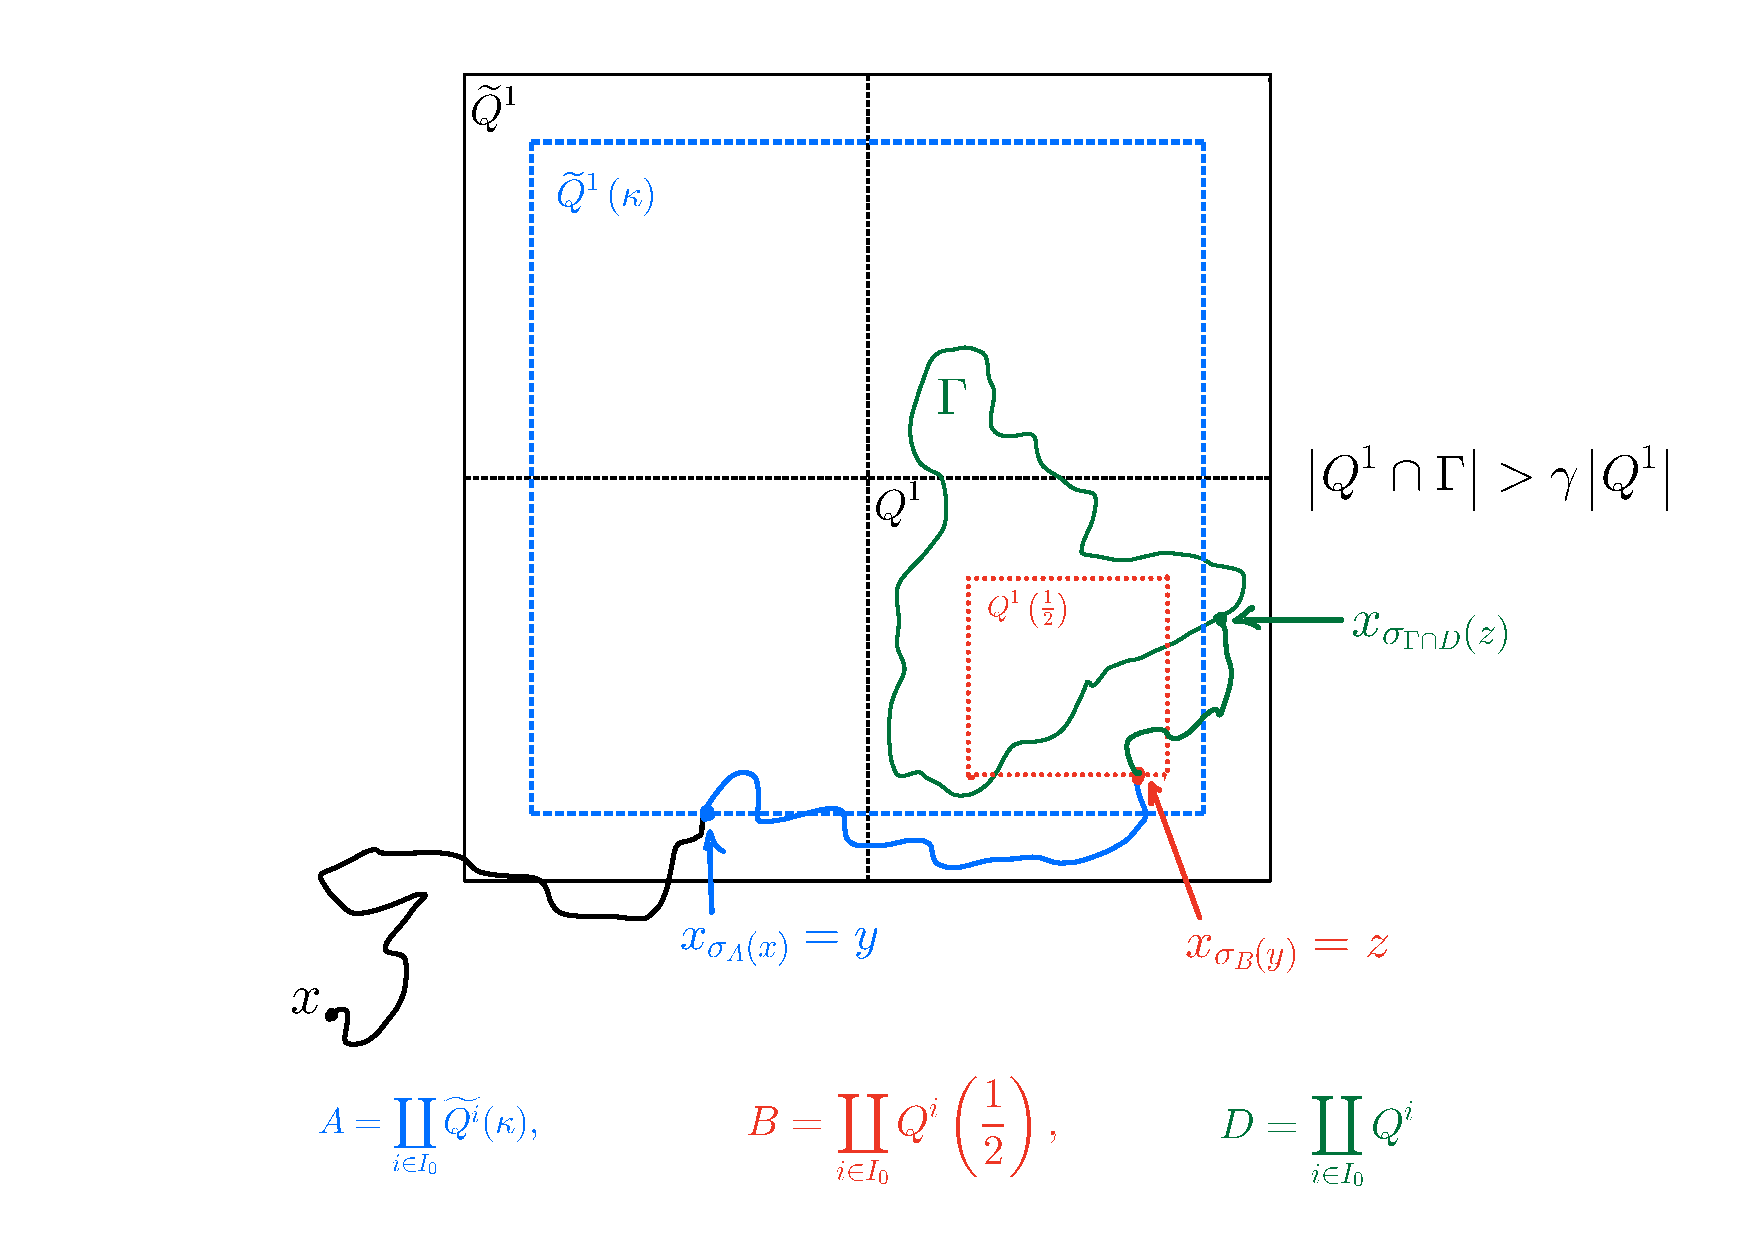
\includegraphics[width=0.9 \textwidth]{hit prob.pdf} 
    \caption{Hitting Prob.} \label{fig:hit} 
    \end{figure}
	
	\section{Harnack Inequality and H\"older estimate}
	In this section, we prove some theorems of Krylov and Safonov \cite{krylov1981certain} concerning (positive) $L$-harmonic functions. Let $\delta\in(0,1)$. Set 
	\begin{align*}
	    \sP(\delta):=\Big\{\{\mP_x\}_{x\in \mR^n}: (\mP_x, X)  \ \textit{is the strong Markov process} \\
        \textit{associate with some } a(\cdot) \in \mS^d_\delta \Big\}.
	\end{align*}
    Let 
    \[
        [u]_{\alpha; D}:=\sup_{x,y\in D} \frac{|u(x)-u(y)|}{|x-y|^\alpha} ~\textit{ and }~ \osc_D u:= \sup_{x\in D} u(x)-\inf_{x\in D} u(x). 
    \]
	
	\begin{theorem}[H\"older estimate]\label{thm:holder}
	  Suppose $u$ is bounded in $Q_1$ and $
	  Lu =0$ in $Q_1$. Then there exist $\alpha$ and $C$ only depending on $d$ and $\delta$ such that
	  \begin{equation}\label{eq:KS-Holder}
	      [u]_{\alpha; Q_{1/2}}\leq C \osc_{Q_1} u.
	  \end{equation} \end{theorem}
	\begin{proof}
  \begin{framed}
      {\bf Claim:} there exists a constant $\rho\in (0,1)$ such that  for any $z\in Q_{1/2}$, $r\leq 1/2$, 
		\begin{equation}\label{eq:osc}
		\osc_{Q_{r/2}(z)} \ u\leq \rho \osc_{Q_{r}(z)} \ u. 
		\end{equation}
  \end{framed}
        Assume the claim is true. Suppose that $x,y\in Q_{1/2}$  and $|x-y|\ll1$, let $k\in \mN$ such that $2^{-k-1}\leq |x-y|< 2^{-k}$. 
        \begin{align*}
            |u(x)-u(y)|\leq& \osc_{Q_{2^{-k}}(x)} u \leq \rho \osc_{Q_{2^{-k+1}}(x)} u \leq \cdots \leq C\rho^k \osc_{Q_1} u\\
            \leq& C \rho^{-\log_2 |x-y|} \osc_{Q_1} u \leq C |x-y|^{-\log_2\rho} \osc_{Q_1} u. 
        \end{align*}
        
        Therefore, the above claim implies \eqref{eq:KS-Holder} with $\alpha=\log_2\rho^{-1}$. 
		
  To prove \eqref{eq:osc}. Without loss of generality, we can assume $\inf_{x\in Q_r(z)}u=0$ and $\sup_{x\in Q_r(z)} u=1$. In this case, $\osc_{Q_{r}(z)} \ u=1$. 
		Let $\Gamma:=\{x\in Q_{r/2}: u(x)\geq 1/2\}$, we may assume $|\Gamma|\geq \frac{1}{2} |Q_{r/2}|$, if not, we replace $u$ by $1-u$. For any $x\in Q_{r/2}$, by  Itô's formula, Theorem \ref{thm:hit} and scaling,  
		\[
            u(x)=\mE_x u(X_{\tau_{Q_r}\wedge \sigma_\Gamma})\geq \frac{1}{2}\mP_x (\sigma_\Gamma<\tau_{Q_{r}})\geq \frac{1}{2} p(2^{-d-1}). 
        \]
        Hence we get 
		$$
		\osc_{Q_{r/2}(z)} u \leq 1-\frac{1}{2}p(2^{-d-1})=:\rho=\rho \osc_{Q_{r}(z)}u. 
		$$
	\end{proof}
	
	
	
	\begin{theorem}[Harnack inequality]\label{thm:harnack}
 Suppose $a\in \mS^d_\delta$ and $L=a_{ij}\p_{ij}$. There exists $C$ depending only on $\delta$ such that if $u$ is nonnegative, bounded in $Q_4$, and $u(X_{t \wedge \tau_{Q_4}})$ is a martingale, then $u(x) \leq C u(y)$ if $x, y \in Q_1$.
    \end{theorem}
    \begin{proof}
        If we look at $u+\delta$ and let $\delta \rightarrow 0$, we may assume $u>0$. By looking at $C u$, we may assume $\inf _{Q_{1/2}} u=1$. By Theorem , we know that $u$ is Hölder continuous in $Q_1$, so there exists
        \[
            y \in Q_{1 / 2} ~\textit{ such that }~ u(y)=1. 
        \]
        We want to show that $u$ is bounded above by a constant in $Q_1$, where the constant depends only on $\delta$.
        
        By the support theorem and scaling, if $x \in Q_{1/2}$, there exists $\delta$ such that 
        \[
            \mathbb{P}_y\left(\sigma_{Q_{1/2}(x)}<\tau_{Q_2}\right) \geq \delta .
        \]
        By scaling, if $z \in Q_{1/2}(x)$, then $\mathbb{P}_z\left(\sigma_{Q_{1/4}(x)}<\tau_{Q_2}\right) \geq \delta$. So by the strong Markov property,
        \[
            \mathbb{P}_z\left(\sigma_{Q_{1/4}(x)}<\tau_{Q_2}\right) \geq \delta^2 .
        \]
        Repeating and using induction,
        \[
            \mathbb{P}_y\left(\sigma_{Q_{2^{-k}}(x)}<\tau_{Q_2}\right) \geq \delta^k .
        \]
        Then
        \[
            \begin{aligned}
                1 & =u(y) \geq \mathbb{E}_y\left[u\left(X_{\sigma_{Q_{2^{-k}}(x)}}\right) ; \sigma_{Q_{2^{-k}}(x)}<\tau_{Q_2}\right] \\
                & \geq \delta^k\left(\inf _{Q_{2^{-k}}(x)} u\right),
            \end{aligned}
        \]
        or 
        \begin{equation}\label{eq:infu-Qk}
            \inf _{Q_{2^{-k}}(x)} u \leq \delta^{-k} , \quad \forall k\geq 1. 
        \end{equation}
        By the proof of Theorem \ref{thm:holder}, there exists $\rho<1$ such that
        \[
             \osc_{Q_{2^{-k-1}}(x)} u\leq \rho \osc_{Q_{2^{-k}}(x)}u .
        \]
        Take $N$ large so that $\rho^{-N} \geq 1/\left(\delta-\delta^2\right)$.  Then
        \[
            \underset{Q_{2^{N-k}}(x)}{\mathrm{Osc}} u \geq \rho^{-N} \underset{Q_{2^{-k}}(x)}{\operatorname{Osc}} u \geq \frac{1}{\delta-\delta^2} \underset{Q_{2^{-k}}(x)}{\operatorname{Osc}} u .
        \]
        Take $K$ large so that $\sqrt{d} 2^{N-K}<1 / 8$. Suppose there exists $x_0 \in Q_1(y)$ such that $u\left(x_0\right) \geq \delta^{-K-1}$. 
        \begin{framed}
            We will construct a sequence $x_1, x_2, \ldots$ by induction such that $u(x_j)\geq \delta^{-K-j-1}$. 
        \end{framed} Suppose we have $x_j \in Q_{2^{N+1-K-j}}\left(x_{j-1}\right)$ with $u\left(x_j\right) \geq \delta^{-K-j-1}$, $j \leq n$. Since $\left|x_j-x_{j-1}\right|<\sqrt{d} 2^{N+1-K-j}, 1 \leq j \leq n$, and $\left|x_0-y\right| \leq 1$, then $\left|x_n-y\right|<2$. Since $u\left(x_n\right) \geq \delta^{-K-n-1}$ and by  \eqref{eq:infu-Qk}, $\inf _{Q_{2^{-K-n}}(x_n)} u \leq \delta^{-K-n}$, 
        $$
            \underset{Q_{2^{-K-n}}(x_n)}{\operatorname{Osc}} u \geq \delta^{-K-n}\left(\delta^{-1}-1\right) .
        $$
        So $\osc_{Q_{2^{N-K-n}}(x_n)} u \geq \delta^{-K-n-2}$, which implies that there exists $x_{n+1} \in$ $Q_{ 2^{N-K-n}}(x_n)$ with $u\left(x_{n+1}\right) \geq \delta^{-K-n-2}$ because $u$ is nonnegative. By induction we obtain a sequence $x_n$ with $x_n \in Q_3(y)$ and $u\left(x_n\right) \rightarrow \infty$. This contradicts the boundedness of $u$ on $Q_4$. Therefore $u$ is bounded on $Q_1$ by $\delta^{-K-1}$.
    \end{proof}
	

\chapter{Divergence Form Operators}

Let \(a\in \mS^d_\delta\). One can also consider the following Dirichlet form 
\[
\cE (u, v) : = \int_{\mR^d} a_{ij} \partial_i u \partial_i v=\cE(v,u), \quad u, v \in H^1. 
\]
Then, 
\[
\cE(u, v) = - \langle Lu, v \rangle=-\< u, Lv \>, \quad u, v \in C_c^\infty, 
\]
where
\[
L u = \partial_j (a_{ij}\partial_i u).
\]
By our assumption on \(a\), 
\[
\cE(u,u)\asymp \int_{\mR^d} |\nabla u|^2 = \|u\|_{H^1}^2. 
\]

\medskip
Assume that \(a\in \mS^d_\delta\cap C^\infty\), and \((\mP_x, X_t)\) be the diffusion process associated to 

For any \(f\in L^1\cap L^\infty\), set \(P_tf(x)=\mE_x f(X_t)\). Then 
\[
\partial_t P_t f = L P_t f, \quad f\in C^\infty_c. 
\]
By the symmetricity of \(L\), we have 
\begin{align*}
    \partial_t\<f,P_t^*g\>=\partial_t\<P_tf,g\>=\<L P_t f, g\>= \<P_tL f, g\>= \<f, LP_t^* g\>, \quad f,g\in C_c^\infty.
\end{align*}
This yields that \(P_t^* f= P_tf\). Consequently, 
\[
\int P_t f = \partial_t \langle P_t f, 1\rangle = \langle f,  P_t 1 \rangle = \int f.
\]



Assume \( f \geq 0 \), \( f\in C_c^\infty \) and \(\|f\|_1 = 1\).

\[
\frac{\d }{\d t} \|P_t f\|_2^2 = \partial_t \langle P_t f, \partial_t P_t f \rangle = 2 \langle P_t f, L P_t f \rangle \leq -2 \delta \| \nabla P_t f \|_2^2
\]
By Nash's inequality: 
\[
\|u\|_2 \leq C(d)\| u \|_1^{\frac{2}{d+2}} \| \nabla u \|_2^{\frac{d}{d+2}}
\] 
and the fact that \(\|P_t f \|_1 \leq \|f\|_1=1\), we obtain
\[
\frac{\d }{\d t} \|P_t f\|_2^2 \leq -c\left( \frac{\|P_t f \|_2}{\|P_t f \|_1^{\frac{2}{d+2}}} \right)^{\frac{2(d+2)}{d}} \leq -c\left( \|P_t f \|_2^2 \right)^{1+\frac{2}{d}}
\]
Put \(\theta(t) = \|P_t f\|^2_2\). Then \(\theta'(t) \leq -c\left(\theta(t)\right)^{1+\frac{2}{d}}\) and \(\theta(t) > 0\). This yields 
\[
\left[ \theta^{-\frac{2}{d}}(t) \right]' \geq c> 0\Rightarrow \theta^{-\frac{2}{d}}(t) \geq ct + \theta^{-\frac{2}{d}}(0). 
\]
Thus, 
\[
\|P_t f\|_2^2 \leq \theta(t) \leq Ct^{-\frac{d}{2}}, \quad \|f\|_1 =1. 
\]
So we obtain 
\begin{equation}\label{eq:L1-to-L2}
    \|P_t\|_{L^1 \to L^2} \leq Ct^{-\frac{d}{4}}
\end{equation}
For any \( f \in L^2, \, g \in L^1 \), 
\[
    \langle P_tf, g \rangle = \langle f, P_t g \rangle \leq C\|f\|_2 \|P_t g\|_2 \leq Ct^{-\frac{d}{4}} \|g\|_1 \|f\|_2. 
\]
This yields 
\begin{equation}\label{eq:L2-to-Linfity}
    \| P_t\|_{L^2 \rightarrow L^\infty} \leq Ct^{-\frac{d}{4}}
\end{equation}
\eqref{eq:L1-to-L2} and \eqref{eq:L2-to-Linfity} imply that 
\[
    \|P_t\|_{L^1 \rightarrow L^\infty} \leq \|P_{\frac{t}{2}}\|_{L^1 \rightarrow L^2} \|P_{\frac{t}{2}}\|_{L^2 \rightarrow L^\infty} \leq Ct^{-\frac{d}{2}}. 
\]
Therefore, 
\[
    p(t,x,y)\leq Ct^{-\frac{d}{2}}. 
\]

\medskip
Set 
\[
P_{t}^{\varphi} f(x) := e^{\varphi (x)} P_{t}(e^{-\varphi} f)(x)
\]
\begin{equation}
    \begin{aligned}
        \langle L^{\varphi} f, g \rangle =& \langle \partial_{t} P_{t}^{\varphi} f, g \rangle|_{t=0} = \langle e^{\varphi} \partial_{t} P_{t}(e^{-\varphi} f), g \rangle|_{t=0}\\
        =& -\int_{\mR^d}a_{ij} \partial_{i} (e^{-\varphi} f) \partial_{j} (e^{\varphi} g) \\
        =& \langle L f, g \rangle + \int a_{ij} (\p_i g\p_j\varphi f-\p_i f\p_j\varphi g) + \int a_{ij} \p_i\varphi \p_j \varphi fg
    \end{aligned}
\end{equation}
\[
\frac{\d }{\d t}\|P_t^\varphi f\|_2^2=\<L^\varphi P^\varphi_t f, P^\varphi_t f\> + \int a_{ij} \p_i\varphi \p_j \varphi f^2. 
\]

Let \(\varphi(x)=\beta\cdot x\) with \(\beta\in \mR^d\), and \(\|f\|_1=1\). Then 
\[
\frac{\d }{\d t}\|P_t^\varphi f\|_2^2\leq C |\beta|^2 \|P_t f\|_2^2 -c\left( \|P_t f \|_2^2 \right)^{1+\frac{2}{d}} 
\]
\[
\theta'(t)\leq C |\beta|^2 \theta(t)-c(\theta(t))^{1+\frac{2}{d}}
\]

\chapter{Appendix}

\section{Probabilistic terminology}
Let $(\Omega, \cF, \bP)$ be a probability space and $(E, \cE)$ be a measurable space. $X:(\Omega,\cF)\to (E, \cE)$ a measurable map, and $\cG$ a $\sigma$-field $\subseteq \cF$.  
	
When $E=\mR$, we define the {\bf conditional expectation}\index{conditional expectation} of $X$ given $\cG$, $\bE(X|\cG)$, to be any random variable $Y$ that satisfies 
\begin{enumerate}[(a)]
    \item $Y\in \cG$; 
    \item for all $A\in \cG$, $\bE(X; A)=\bE(Y; A)$. 
\end{enumerate}
	
$Q_{\cG}: \Omega\times \cE\to [0,1]$ is said to be a {\bf {regular conditional distribution}\index{regular conditional distribution (probability)}} (RCD) for $X$ given $\cG$ if 
\begin{enumerate}[(a)]
    \item For each $A\in \cE$, $\omega\mapsto Q_{\cG}(\omega, A)$ is a version of $\bE(\1_A(X)|\cG)$; 
    \item For a.e. $\omega\in \Omega$, $A\mapsto Q_{\cG}(\omega, A)$ is a probability measure. 
\end{enumerate}
If $E=\Omega$, $X(\omega)=\omega$, then $Q_{\cG}$ is called a {\bf regular conditional probability}. 
	
The following results can be found in Durrett's book \cite{durrett2019probability}.  
\begin{proposition}
    \begin{enumerate}[(i)]
	\item If $\cG_1\subseteq \cG_2\subseteq \cF$, then 
	\begin{equation}
		\bE[(X|\cG_2)|\cG_1]=\bE (X|\cG_1)
	\end{equation}
	\item Assume that $X\in \cF$ and $Y\in \cG\subseteq \cF$, then 
	\begin{equation}
		\bE (XY|\cG)=\bE (X|\cG)Y. 
	\end{equation}
	\item (Jesen's inequality) If $\varphi$ is a convex function, then 
	\begin{equation}
		\bE (\varphi(X)|\cG) \leq \varphi(\bE (X|\cG)). 
	\end{equation}
    \end{enumerate}
\end{proposition}
	
\begin{proposition}
    Let $Q_{\cG}$ be a RCD for $X$ given $\cG$. If $f:E\to \mR$ satisfying $\bE |f(X)|<\infty$, then 
    \[
	\bE(f(X)|\cG)(\omega)= \int_{E} f(x) Q_{\cG}(\omega, \d x)\quad a.s.. 
    \]
\end{proposition}
	
\begin{theorem}
    RCD exists if $E$ is a {\bf standard measure space} and $\cE=\cB(E)$. 
\end{theorem}
	
\begin{proposition}
    Assume $X\geq 0$, $f:\mR_+\to \mR_+$ such that $f\in C^1(\mR_+)$ and $f(0)=0$. Then 
    \begin{equation}
	\bE f(X)= \int_0^\infty f'(t) \bP (X>t) \d t. 
    \end{equation}
\end{proposition}
\begin{exercise}
    If $X\geq 0$, $f:\mR_+\to \mR_+$ such that $f\in C^1(\mR_+)$ and $f(\infty)=0$. Then 
    \begin{equation}
	\bE f(X)= -\int_0^\infty f'(t) \bP (X\leq t) \d t. 
    \end{equation}
\end{exercise}

\section{Maximal Principle}
Consider the linear parabolic equation:
\[
    \partial_t u = a_{ij}\partial_{ij} u + b_i\partial_i u + cu,
\]
where \(a_{ij}\) is uniformly elliptic, \(b_i\) and \(c\) are bounded and continuous. 

\begin{proposition}[Weak Maximum Principle]
    If \(c(x, t) \leq 0\) and \(u\) is bounded, then 
    \[
    \sup_{\mR_+\times\mathbb{R}^d} u = \sup_{\{0\}\times\mathbb{R}^d} u.
    \]
\end{proposition}
\begin{proposition}[Strong Maximum Principle]
    If \(u\) achieves its maximum (or minimum) at a point \((t_0,x_0) \in \mR_+\times \mathbb{R}^d\), then \(u\) is constant in \([0, t_0]\times\mathbb{R}^d\).
\end{proposition}

\section{Schauder estimate}\label{app:Schauder}

Let $\sS$ be the Schwartz space of all rapidly decreasing functions, and $\sS'$ the dual space of $\sS$ called Schwartz generalized function (or tempered distribution) space. Given $f\in\sS$,
let $\sF f=\hat f$  be the Fourier transform defined by
$$
    \hat f(\xi):=\int_{\mR^d}\e^{-\mathrm{i}2\pi\xi\cdot x} f(x)\d x.
$$
Let $\chi:\mR^d\to[0,1]$ be a smooth radial function with 
$$
\chi(\xi)=1,\ |\xi|\leq 1,\ \chi(\xi)=0,\ |\xi|\geq 3/2.
$$
Define
$$
\varphi(\xi):=\chi(\xi)-\chi(2\xi).
$$
It is easy to see that $\varphi\geq 0$ and supp $\varphi\subset B_{3/2}\setminus B_{1/2}$ and formally 
\begin{align}\label{EE1}
    \sum_{j=-k}^k\varphi(2^{-j}\xi)=\chi(2^{-k}\xi)-\chi(2^{k+1}\xi)\stackrel{k\to\infty}{\to} 1.
\end{align}
In particular, if $|j-j'|\geq 2$, then
$$
\mathrm{supp}\varphi(2^{-j}\cdot)\cap\mathrm{supp}\varphi(2^{-j'}\cdot)=\varnothing.
$$
From now on we shall fix such $\chi$ and $\varphi$ and define
$$
\Delta_j f:=\sF^{-1}(\varphi(2^{-j}\cdot) \sF f), \quad j\in \mZ.
$$
Set \(h:=\sF^{-1}(\varphi)\), then \(h_j := \sF^{-1}(\varphi (2^{-j}\cdot))= 2^{jd} h(2^j \cdot)\). Noting that we have 
\[
    \int_{\mR^d} h_j =\varphi(0)=0.  
\]
        
We first recall the following useful lemmas. 
\begin{lemma}\label{lem:Besov-Holder}
    Let $\alpha\in (0,1)$. For any $u\in C^\alpha$, it holds that 
    \begin{align}\label{Ch}
	\frac{1}{C}\sup_{j\in \mZ} 2^{j\alpha} \|\Delta_j u\|_0\leq [u]_{\alpha} \leq C \sup_{j\in \mZ} 2^{j\alpha} \|\Delta_j u\|_0, 
    \end{align}
    where 
    \[
	[u]_\alpha:= \sup_{x\neq y} \frac{|u(x)-u(y)|}{|x-y|^\alpha}, 
    \]
    and $C$ only depends on $d$ and $\alpha$. 
\end{lemma}
\begin{proof}
    1) For any \(x\neq y\), we have 
    \begin{align*}
        |u(x)-u(y)| \leq& \sum_{j} |\Delta_j u(x)-\Delta_j u(y)| \leq \sum_j (|x-y|\|\nabla \Delta_j u\|_{0}) \wedge (2 \|\Delta_j u\|_0)\\
        \leq& C\sum_{j} (2^j|x-y|\wedge 1) \|\Delta_j u\|_0 \\
        %\leq& C |x-y|^\alpha \sup_{j} 2^{j\alpha}\|\Delta_j u\|_0 \sum_{j} (2^{j(1-\alpha)} |x-y|^{1-\alpha} \wedge 2^{-j\alpha} |x-y|^{-\alpha}) \\
        \leq & C 2^{j\alpha}\|\Delta_j u\|_0  \l( |x-y| \sum_{j\leq \log_2 |x-y|} 2^{j(1-\alpha)}+ \sum_{j\geq \log_2 |x-y|} 2^{-j\alpha} \r) \\
        \leq & C |x-y|^\alpha \sup_{j} 2^{j\alpha} \|\Delta_j u\|_0. 
    \end{align*}
    
    2) For any \(j\in \mZ\) and \(x\in \mR^d\), we have 
    \begin{align*}
        |\Delta_j u(x)|=& \l| \int_{\mR^d}  u(x-y) h_j(y) \d y \r|= \l| \int_{\mR^d} [u(x-y)-u(x)] h_j(y) \d y \r| \\
        \leq & [u]_\alpha 2^{jd} \int_{\mR^d} |y|^{\alpha} |h(2^{j}y)| \d y \leq C 2^{-j\alpha} [u]_\alpha. 
    \end{align*}
\end{proof}
	
\begin{lemma}\label{lem:schauder}
    There is a constant $C=C(d, \alpha)$, such that for any $u\in C^{2,\alpha}$ and \(\lambda \geq 0\), 
    \begin{equation}
        \lambda \|u\|_0\leq C \|\lambda u-\Delta u\|_0
    \end{equation}
    and 
    \begin{equation}
        \lambda [u]_\alpha+[\nabla^2 u]_\alpha \leq C [\lambda u- \Delta u]_\alpha
    \end{equation}
\end{lemma}
\begin{proof}
    1) If there exits \(x_0\in \mR^d\) such that \(u(x_0) ( \mbox{ or }-u(x_0))=\|u\|_0\), then \(\Delta u(x_0) \leq 0~ (\Delta u(x_0)\geq 0)\). This implies 
    \(|\lambda u(x_0)|\leq |\lambda u(x_0)-\Delta u(x_0)|\); If such \(x_0\) does not exist, then we can consider function \(u_R= u \chi(\cdot/R)\) (\(R\gg 1\)). 
    
    2) We only prove the case \(\lambda=0\). Let \(f=\Delta u\). Define 
    $$
        \varphi^{kl} (\xi):= \frac{\xi_k\xi_l}{|\xi|^2} \varphi (\xi),\ \  h^{kl}(x):=\sF^{-1}(\varphi^{kl})(x);  \ \ \varphi^{kl}_j (\xi):= \varphi^{kl}(2^{-j}\xi), \ \ h^{kl}_j(x):=2^{jd} h^{kl}(2^jx). 
    $$
    It is easy to see
    $$
        \p_{kl}u=\sum_{j\in \mZ} u^{kl}_j:=\sum_{j\in \mZ}\varphi^{kl}_j (D) f=\sum_{j\in \mZ} h^{kl}_j* f.  
    $$
    For any $x\in \mR^d$, noticing $h^{kl}\in \sS(\mR^d)$ and $\int h^{kl}=\varphi (0)=0$, we get 
    \begin{align*}
        |u^{kl}_j(x)|=&\left|\int_{\mR^d} h^{kl}_j (y)f(x-y) \d y\right|=\left|\int_{\mR^d} h^{kl} (z)(f(x-2^{-j}z)-f(x)) \d z\right| \\
        \leq&  \int_{\mR^d} |h^{kl}(z)| \cdot [f]_\alpha |2^{-j}z|^\alpha  \d z\leq C [f]_\alpha 2^{-j\alpha}
    \end{align*}
    This together with \Cref{lem:Besov-Holder} yields that  
    \[
        [\nabla^2 u]_\alpha \leq C\sup_{j,k,l}2^{j\alpha}\|\Delta_j \partial_{kl}u\|_0 \leq C [f]_\alpha. 
    \]
\end{proof}


\section{Monge-Ampère Equation}\label{app:MAE}

\begin{lemma}[Area formula]
    Consider a locally Lipschitz function $f: \mR^d \to \mR^d$ and a Borel set $A\subseteq \mR^d$. Then the function $y\mapsto N_A(y):= \mathrm{card}\{f^{-1}(y)\cap A\}\}$ is measurable and 
    \begin{equation*}
        \int_{A} |\det (\nabla f(x))| \d x = \int_{\mR^n} N_A(y) \d y \geq \sL^d(f(A)). 
    \end{equation*}
    Consequently, for any $g\geq 0$, 
    \begin{equation}\label{eq:area}
        \int_{f(A)}g(y)\d y\leq \int_{A} g(f(x)) |\det \nabla f(x)|\d x. 
    \end{equation}
\end{lemma}
        
To motivate the definition of weak solutions to \eqref{eq:MAE}, given an open set $D \subset \mathbb{R}^n$, consider $u: D \rightarrow \mathbb{R}$ a convex function of class $C^2$ satisfying \eqref{eq:MAE} 
	for some $f: D \rightarrow \mathbb{R}^{+}$. Then given any Borel set $E \subset D$, it follows by the area formula that
	$$
	\int_E f \,\d x=\int_E \operatorname{det} D^2 u\, \d x=|\nabla u(E)| .
	$$
	
	Notice that while the above argument needs $u$ to be of class $C^2$, the identity
	$$
	\int_E f=|\nabla u(E)|
	$$
	makes sense if $u$ is only of class $C^1$. To find a definition when $u$ is merely convex one could try to replace the gradient $\nabla u(x)$ with the subdifferential $\partial u(x)$ and ask for the above equality to hold for any Borel set $E$. Here $\p u(x)$ is given by 
	$$
	\partial u(x):=\left\{p \in \mathbb{R}^d: u(y) \geq u(x)+\langle p, y-x\rangle \quad \forall y \in D\right\}. 
	$$
	This motivates the following definition:
	\begin{definition}
		Given an open set $D \subset \mathbb{R}^n$ and a convex function $u: D \rightarrow \mathbb{R}$, we define the Monge-Ampère measure associated to $u$ by
		$$
		\mu_u(E):=\left|\bigcup_{x \in E} \partial u(x)\right|
		$$
	\end{definition}
	The basic idea of Alexandrov was to say that $u$ is a weak solution
	of \eqref{eq:MAE} if $\mu_u|_{D}=\nu|_{D}$. 
	
	\begin{lemma}
		Let $u,v:D\to \mR$ be convex functions. Then 
		$$
		\mu_{u+v} \geq \mu_u+\mu_v \quad \text { and } \quad \mu_{\lambda u}=\lambda^n \mu_u \quad \forall \lambda>0 .
		$$
	\end{lemma}
	
	\medspace
	
	The following result is  the celebrated Alexandrov maximum principle.
	\begin{theorem}
		Let $D$ be  an open bounded convex set, and let $u: D\to \mR$ be a convex function such that $u|_{\p D}=0$. Then there exists a dimensional constant $C=C(d)$
		such that 
		\begin{equation}\label{eq:abp}
			|u(x)| \leq C(d) \operatorname{diam}(D)^{\frac{d-1}{d}} \operatorname{dist}(x, \partial D)^{\frac{1}{d}}|\partial u(D)|^{\frac{1}{d}},  \quad \forall x \in D. 
		\end{equation}
	\end{theorem}
	\begin{proof}
		Let $(x, u(x))$ be a point on the graph of $u$, and consider the convex ``conical" function $y\mapsto \widehat C_x(y)$ with vertex at $(x, u(x))$ that vanishes on $\p D$. 
		Since $u\leq \widehat C_x$ in $D$ (by the convexity of $u$), Lemma 2.7 implies that 
		$$
		\left|\partial \widehat{C}_x(x)\right| \leq\left|\partial \widehat{C}_x(D)\right| \leq|\partial u(D)| ;
		$$
		so, to conclude the proof, it suffices to bound $|\p \widehat C_x(x)|$ from below. It is not hard to see 
		\begin{itemize}
			\item $\p \widehat{C}_x(x)$ contains the ball $B_\rho$ with $\rho=|u(x)|/\mathrm{diam} (D)$
			\item $\p \widehat{C}_x(x)$ contains a vector of norm $|u(x)|/\mathrm{dist} (x, \p D)$
		\end{itemize}
		Thus, 
		$$
		\partial \widehat{C}_x(x) \supset B_{\varrho}(0) \cup\{q\}, \quad |q|=|u(x)|/\mathrm{dist} (x, \p D). 
		$$
		Since $\p \widehat{C}_x(x)$ is convex, it follows that $\p \widehat{C}_x(x)$ contains the cone $\cC$ generated
		by $q$ and $\Sigma_q:= \{p\in B_\rho: \<p,q\>=0\}$. Therefore 
		$$
		c(d) \rho^{d-1} |q| = |\cC| \leq |\p u(D)|. 
		$$
	\end{proof}
	
	\begin{theorem}
		Let $D$ be an open bounded convex set, and let $\nu$ be a Borel measure on $D$ with $\nu(D)<\infty$. Then there exists a unique convex function $u: D \rightarrow \mathbb{R}$ solving the Dirichlet problem
		$$
		\begin{cases}
			\mu_u=\nu & \text { in } D \\ u=0 & \text { on } \partial D
		\end{cases}
		$$
	\end{theorem}
	
	\begin{proof}
		By the stability result proved in Lemma below, since any finite measure can be approximated in the weak*
		topology by a finite sum of Dirac deltas, we only need to
		solve the Dirichlet problem  when $\nu=\sum_{i=1}^N \alpha_i \delta_{x_i}$ with $x_i\in D$ and $\alpha_i>0$. To prove existence of a solution, we use the so-called Perron method: we define 
		$$
		\mathcal{S}[\nu]:=\left\{v: \Omega \rightarrow \mathbb{R} \text { convex : }\left.v\right|_{\partial \Omega}=0, \mu_v \geq \nu \text { in } \Omega\right\}
		$$
		and we show that the largest element in $\cS[\nu]$ is the desired solution. We split the argument into several steps.
		
		{\em Step 1}: $\cS[\nu]\neq \emptyset$. To construct an element of $\cS[\nu]$, we consider the ``conical" function $C_{x_i}$, that is $0$ on $\p\Omega$ and takes the value $-1$ at its vertex $x_i$. The Monge–Ampère measure of this function is concentrated at $x_i$ and has mass equal
		to some positive number $\beta_i$ corresponding to the measure of the set of supporting hyperplanes at $x_i$. Now, consider the convex function $\bar v=\sum_{i=1}^N \lambda C_{x_i}$, where $\lambda$ has to be chosen.
		We notice that $\bar v|_{\p \Omega}=0$. In addition, provided $\lambda$ is sufficiently large, Lemma below  
		implies that 
		$$
		\mu_{\bar{v}} \geq \sum_{i=1}^N \mu_{\lambda \hat{C}_{x_i}}=\sum_{i=1}^N \lambda^d \mu_{\hat{C}_{x_i}}=\sum_{i=1}^N \lambda^d \beta_i \delta_{x_i} \geq \sum_{i=1}^N \alpha_i \delta_{x_i} = \nu.
		$$
		This yields $\bar v\in \cS[\nu]$. 
		
		{\em Step 2}: $v_1, v_2 \in \mathcal{S}[\nu] \Rightarrow w:=\max \left\{v_1, v_2\right\} \in \mathcal{S}[\nu]$. Set 
		$$
		\Omega_0:=\left\{v_1=v_2\right\}, \quad \Omega_1:=\left\{v_1>v_2\right\}, \quad \text { and } \quad \Omega_2:=\left\{v_1<v_2\right\}
		$$
		Also, given a Borel set $E\subseteq \Omega$, consider $E_i= E\cap \Omega_i$. 
		
		Since $\Omega_1$ and $\Omega_2$ are open sets, $w|_{\Omega_1}=v_1$ and $w|_{\Omega_2}=v_2$, 
		$$
		\p w(E_1) = \p v_1(E_1), \quad   \p w(E_2) = \p v_2(E_2). 
		$$
		In addition, since $w=v_1$ on $\Omega_0$ and $w\geq v_1$ everywhere else, we have 
		$$
		\p v_1(E) \subseteq \p w(E_0). 
		$$
		Therefore, 
		$$
		\mu_w (E) \geq \mu_{v_1}(E_0\cup E_1)+ \mu_{v_2} (E_2) \geq \nu(E).  
		$$
		
		{\em Step 3}: $u:=\sup _{v \in S[\nu]} v$  belongs to  $S[\nu]$. Let $w_m \uparrow u$ locally uniformly. Then $\mu_{w_m} \rightharpoonup*\mu_u$.  Also, we deduce
		immediately that $u|_{\p\Omega}=0$ by construction;  hence, $u\in \cS[\nu]$. 
		
		{\em Step 4}: The measure $\mu_u$ is supported at the points $\{x_1,\cdots x_N\}$. Otherwise, there exists a set $E\subseteq D$ such that
		$$
		E \cap\left\{x_1, \ldots, x_N\right\}=\emptyset \quad \text { and } \quad|\partial u(E)|=\mu_u(E)>0
		$$
		Therefore, 
		$$
		\l|\partial u(E)\backslash [\cup_{i=1}^{N} \p u(x_i)\cup \p u(\p D)]\r|=|\p u (E)|>0 
		$$
		Let $x_0\in E$ and $p\in \p u(x_0)\backslash [\cup_{i=1}^{N} \p u(x_i)\cup \p u(\p D)]$. Then there exists $\delta>0$ such that
		\begin{equation}\label{eq:baru}
			u \geq \ell_{x_0, p}+2 \delta \quad \text { on }\left\{x_1, \ldots, x_N\right\} \cup \partial \Omega, 
		\end{equation}
		
		where $\ell_{x_0, p}(x)=u(x_0)+p\cdot (x-x_0)$. Set $\bar{u}:=\max\{\ell_{x_0, p}+\delta, u\}\gneqq u$. Notice that $\bar{u}$ is convex, $\bar{u} \geqslant u$, and it follows by \eqref{eq:baru} that $\bar{u}=u$ in a neighborhood of $\left\{x_1, \ldots, x_N\right\} \cup \partial \Omega$. In particular, $\left.\bar{u}\right|_{\partial \Omega}=0$ and $\partial \bar{u}\left(x_i\right)=\partial u\left(x_i\right)$, which implies that $u\log eqq\bar u\in \cS[\nu]$. This is a contradiction. 
		
		{\em Step 5}: $\mu_u=\nu$. By {\em Step 3} and {\em Step 4}, we know that $\mu_{u}=\sum_{i=1}^N \beta_i \delta_{x_i}$ with $\beta_i\geq \alpha_i$. Assume that $\beta_1=\mu_u(x_1)>\nu(x_1)=\alpha_1$. 
\end{proof}

\bibliographystyle{alpha} 
\bibliography{mybib}

%\backmatter
%\include{index}

\end{document}

%-----------------------------------------------------------------------
% End of chapter.tex
%-----------------------------------------------------------------------
